\documentclass[a4paper]{memoir}
\usepackage[utf8]{inputenc}
\usepackage{OldStandard}
% \usepackage{lmodern}
\usepackage{microtype}

\usepackage[dvipsnames]{xcolor}
\usepackage{amsmath}
\usepackage{amsfonts}
\usepackage{amsthm}
\usepackage{commath}
\usepackage{mathtools}
\usepackage{siunitx}
\DeclareSIUnit\year{yr}
\DeclareSIUnit\litre{\liter}

\usepackage{tikz}
\usetikzlibrary{angles,quotes}
\usepackage{pgfplots}
\pgfplotsset{compat=1.14}
\usepgfplotslibrary{polar}
\usepackage{graphicx}
\usepackage{sidecap}
\sidecaptionvpos{figure}{c}
\usepackage{float}
\usepackage{hyperref}
\usepackage{enumitem}
\usepackage{wasysym}
\usepackage{multicol}
\usepackage{tabularx}
\usepackage{titlesec}
\usepackage[framemethod=tikz]{mdframed}
\usepackage{cancel}
\usepackage{chngcntr}

% \renewcommand*{\thefootnote}{\fnsymbol{footnote}}

\newtheorem*{thm}{Theorem}
\newtheorem*{iden}{Identity}
\newtheorem*{lemma}{Lemma}
\theoremstyle{definition}
\newtheorem*{defn}{Definition}
\newtheorem*{joke}{Joke}
\newtheorem*{app}{Application}
\newtheorem*{ex}{Example}
\newtheorem*{pro}{Problem}
\newtheorem*{exs}{Examples}


% \newtheorem*{PRIVATEexercises}{Exercises}
%
% \newlist{subexercises}{enumerate}{4}
%
% \setlist[subexercises,1]{
%   label=\arabic*.,
%   before=\setcounter{subexercisesi}{\value{subexercises}},
%   after=\setcounter{subexercises}{\value{subexercisesi}},
% }% ALWAYS resumed
% \setlist[subexercises,2]{label=(\alph*)}%           NOT resumed
% \setlist[subexercises,3]{label=(\roman*)}%           NOT resumed
% \setlist[subexercises,4]{label=(\greek*)}%           NOT resumed
%
% \newcounter{subexercises}
%
% \newenvironment{exercises}{
%     \begin{mdframed}\begin{PRIVATEexercises}\leavevmode
%     \begin{subexercises}
%   }
%   {
%     \end{subexercises}
%     \end{PRIVATEexercises}\end{mdframed}
% }

% russian integral
\usepackage{scalerel}
\DeclareMathOperator*{\rint}{\scalerel*{\rotatebox{17}{$\!\int\!$}}{\int}}

\setlrmarginsandblock{3.5cm}{2.5cm}{*}
\setulmarginsandblock{2.5cm}{*}{1}
\checkandfixthelayout

\counterwithout{section}{chapter}
\renewcommand{\thechapter}{\Roman{chapter}}
\renewcommand{\thesection}{\thechapter.\arabic{section}}

\setlength\cftsectionnumwidth{2.5em}

\newlength\drop
\newcommand*{\titleGM}{\begingroup% Gentle Madness
\drop = 0.1\textheight
\vspace*{\baselineskip}
\vfill
  \hbox{%
  \hspace*{0.2\textwidth}%
  \rule{1pt}{\dimexpr\textheight-35pt\relax}%
  \hspace*{0.05\textwidth}%
%\fbox{%
\parbox[b]{0.75\textwidth}{
  \vbox{%
    \vspace{\drop}
    {\noindent\HUGE\bfseries Level Three\\[0.5\baselineskip] Calculus}\\[2\baselineskip]
    {\Large\itshape Second Edition}\\[4\baselineskip]
    {\Large ALEX ELZENAAR}\par
    \vspace{0.5\textheight}
    {\noindent \url{https://github.com/aelzenaar/ncea-notes}}\\[\baselineskip]
    }% end of vbox
}% end of parbox
%}% end of fbox
  }% end of hbox
\vfill
\null
\endgroup}

\title{Introduction to Calculus}
\author{Alex Elzenaar}
\date{\today}

\begin{document}

\frontmatter

\begin{titlingpage}
  \titleGM
\end{titlingpage}


\chapter{Preface for the navigator}
These notes are my second attempt at a coherent introduction to calculus at the level of NCEA
Level 3 and NZ Scholarship.

I have made a few philosophical changes from the first edition:-
\begin{itemize}
  \item I treat anti-differentiation at the same time as differentiation. (I do introduce the $ \rint $ notation
        and the term `indefinite integral' here, though I would rather not.)
  \item The notes are split into ``topic'' chapters: \textit{The basics} (the basic formal manipulations
        of derivatives and anti-derivatives), \textit{Geometry of curves} (studying curves via differentiation),
        \textit{Geometry of spaces} (definite integrals, the fundamental theorem of calculus, and arc lengths,
        surface area, and volumes), and \textit{Motion and change} (differential equations).
  \item I have dropped many of the proofs; my justification for this change is threefold(!). Firstly,
        the students that `need' the proofs will see them in a Stage I university course. Secondly, many
        of the proofs in elementary calculus often obscure a nugget of geometry behind the formal manipulation
        of limits, and so I would rather include intuitive geometric \emph{justifications} for results in the
        space the proofs formerly were. Finally, most students at Level 3 are simply not ready for proofs: either
        they don't understand why proof is required, or their level of mathematical sophistication means that
        the proofs seem esoteric. I have included copious references to textbooks where proofs can be found.
  \item I have dropped one or two rather esoteric and old fashioned topics that I used to teach to scholarship
        students; most prominently, trig substitution. These have been replaced with a couple of new topics; one
        in particular is a much expanded explanation of Taylor polynomials (\emph{not} Taylor series!). Note also
        that the main application of trig substitution is to integrate all rational functions: we expand our
        expression into its partial fraction form, we can integrate the terms with linear denominators easily, and
        then we need trig substitution to integrate the quadratic denominators. But after covering the L3 algebra
        topic (in particular, one needs to justify quickly something like $ \mathrm{cis}(z) = \exp(iz) $) then it
        is possible to integrate these terms by factorising them into (complex) linear terms.
\end{itemize}

I feel the need also to point out that these notes are incredibly geometric. \emph{If you don't like teaching geometry, these are not the notes for you.}

\section{Prerequisite material}
Firstly, a hard fact: for a student to be successful in L3 calculus, they should have
a good understanding of the material at L2 and earlier (I would generally expect that
students with less than a merit in the level 2 algebra standard will struggle).

In these notes, I will use material from algebra and geometry at L2 or earlier liberally;
I try to point it out when I use some of the more obsure results. I do not use any
material from any of the level three standards, except trigonometry.

So, in general, the prerequisites and expectations for these notes are:-
\begin{itemize}
  \item A good understanding of L2 coordinate geometry and algebra.
  \item A decent understanding of L3 trigonometry, \emph{including the manipulation of identities}.
\end{itemize}

For some of the sections, knowledge of a little physics (L1 and/or L2) would be nice. I cover
the material in the L2 calculus standard quickly so this is not formally a prerequisite, but a student
who doesn't understand the material there well will struggle with these notes. Roughly speaking,
the differentiation material there is more important.

I would strongly recommend revising the material on functions (section 4 of my own level 2 notes).

\section{Recommended textbooks}
I have used the following textbooks when writing these notes, in roughly increasing order of sophistication:
\begin{itemize}
  \item \emph{Calculus made easy}, by Sivanus P. Thompson and Martin Gardner. This book is perhaps at the correct level mathematically speaking
        for a Y12/13 student, but it is not very geometric. It is certainly worth looking at, though.
  \item \emph{Calculus}, by James Stewart. This is one of the standard first-year computational calculus books. It has many examples and many exercises,
        but lacks soul.
  \item \emph{Calculus}, by Michael Spivak. This is often called the `One True Calculus Book',\footnote{For example, by the \emph{Chicago undergraduate
        mathematics bibliography}: \url{https://www.ocf.berkeley.edu/~abhishek/chicmath.htm} (somewhat useful, if taken with a grain of salt).} but
        is more properly an introduction to real analysis. As such, it is too diffcult for all but the most motivated high school students.
  \item (For the sake of completeness,) \emph{Advanced Calculus}, by L. H. Loomis and S. Sternberg. This is the author's favourite calculus
        book, but is eminently unsuitable for high school students of any motivation.
\end{itemize}

\chapter{Preface for the student}
\begin{figure}
  \centering
  
\includegraphics[width=0.8\textwidth]{hobbes}
\end{figure}
I don't have much to say, really. I could spend time explaining why calculus is useful, but I won't do that here because we'll see
a lot of examples of calculus `in the wild' as we progress (just as a taster, we'll look at some physics, some biology, some economics,
and maybe even some statistics). I could equally well spend time trying to explain exactly what calculus \emph{is} exactly, but this
page is not large enough to contain such an exposition.

Instead, I will give some study advice.

Firstly, you must read the notes. You must sleep with them beneath your pillow. You must work through the examples yourself. You must
do all the problems. You must ask questions.

Because no student ever follows my first piece of advice, I will give you a second, easier option. For each topic, there are a few
homework problems set. \emph{At a minimum}, you should do all these problems. (But beware, if you \emph{only} do these problems, you
will be woefully underprepared for any situation you need calculus for.)

Secondly, draw pictures. I do my best to include lots of diagrams (some even in colour!), but one can never have too many
pictures. (As a young girl called Alice once perceptively remarked, ``What is the use of a book without pictures or
conversations?''\footnote{\emph{Alice in Wonderland}, by Lewis Carroll.})

Thirdly, and I cannot stress this enough, \emph{your exam grades do not matter}.$^\textit{[citation needed]}$ It is perfectly possible to pass calculus exams
without understanding the material, but if you do that (by, for example, trying to memorise everything in leu of understanding it),
you are cheating yourself out of an education. If you understand the material, you will be prepared for every subject you may wish
to take next year (and, as a bonus, you'll pass the exam).

Let us begin.

\cleardoublepage
\begin{KeepFromToc}
\tableofcontents*
\end{KeepFromToc}

\mainmatter

\counterwithout{figure}{chapter}
\counterwithout{table}{chapter}

\chapter{The basics}

\section{Tangent lines}
Suppose we have two variables, $ y $ and $ x $, such that any change in $ x $ produces
a corresponding change in $ y $. In the language we learned last year, we say that $ y $
is a function of $ x $: that is, there is a function $ f $ such that $ y = f(x) $.

Let us look at a few different functions.

\begin{figure}\centering
  \begin{tikzpicture}
    \begin{axis}[
        axis lines = center,
        xlabel = $ x $,
        ylabel = {$ y = x^2 + x - 1 $}
      ]
        \addplot[domain = -5:5, color = red] {x^2 + x - 1};
    \end{axis}
  \end{tikzpicture}
  \caption{A parabola, $ y = x^2 + x - 1 $.\label{fig:func1}}
\end{figure}

Firstly, let's consider the function $ f $ defined by $ f(x) = x^2 + x - 1 $, graphed in figure \ref{fig:func1}. Let's
look at how $ f $ behaves at a point $ x_0 $ by adding a small number $ h $ to the input and seeing how it changes
the output.

\begin{displaymath}
  f(x_0 + h) = (x_0 + h)^2 + (x_0 + h) - 1 = x_0^2 + 2x_0 h + h^2 + x_0 + h - 1.
\end{displaymath}

We're actually interested in the difference between our new output and our old output, because this gives us
a measure of how quickly $ f $ changes when we move along the $ x$-axis by $ h $.

\begin{displaymath}
  f(x_0 + h) - f(x_0) = (x_0^2 + 2x_0 h + h^2 + x_0 + h - 1) - (x_0^2 + x_0 - 1) = 2x_0 h + h + h^2
\end{displaymath}

If $ h $ is small, then $ h^2 $ is miniscule and only makes up a very small part of $ f(x_0 + h) $. We can therefore
make the following approximation:
\begin{displaymath}
  f(x_0 + h) - f(x_0) \approx (2x_0 + 1)h.
\end{displaymath}
In other words, a small change in the input from $ x_0 $ to $ x_0 + h $ produces a change in the output of the form $ (2x_0 + 1)h $.

When we looked at straight lines in the past, they had a measure of \emph{slope}: the ratio of `rise' (change in output) to `run'
(change in input). For each $ x_0 $ that we feed into $ f $ here, we have a measure of the `rise' of $ f $ over a very small distance, $ h $.
It makes sense, then, to define the slope of $ y = f(x) $ at $ x_0 $ to be $\text{rise}/\text{run}$:
\begin{equation}
  \frac{f(x_0 + h) - f(x_0)}{h} \approx \frac{(2x_0 + 1)h}{h} = 2x_0 + 1
\end{equation}
So when $ h $ is very small, the graph of $ f $ between $ x_0 $ and $ x_0 + h $ looks like a straight line with slope $ 2x_0 + 1 $.

Since the slope of our function defined in this way depends on the value of $ x_0 $, we have a new function which assigns to each point $ x_0 $
the slope of $ f $ around $ x_0 $. We denote this function by $ f' $, and call it the \emph{derivative} of $ f $. The slope of $ f $ at $ x_0 $
will be written $ f'(x_0) $.

Another notation for the derivative is also common; because we are looking at changes in $ y $ divided by changes in $ x $ it sometimes
makes sense to write the derivative as $ \od{y}{x} $ (where $ \dif{x} $ denotes, in some sense, a small change in $ x $). The value of the
derivative at $ x_0 $ is written as $ \eval{\dod{y}{x}}_{x = x_0} $. This notation is known as Leibniz notation, as it was first introduced
in the 1600s by Gottfried Leibiz (a German mathematician and philosopher who, it can be argued, was one of the first modern mathematicians
to develop calculus in a sophisticated manner).

The derivative of the derivative of $ f $ is called the second derivative of $ f $, and we write $ f'' $ for this new function. In general,
the $ n$th derivative of $ f $ is denoted by $ f^{(n)} $ (it is the function produced by repeatedly differentiating $ f $). In Leibniz
notation, the $ n$th derivative of $ y = f(x) $ is $ \od[n]{y}{x} $.

\begin{defn}
  \begin{enumerate}
    \item If we can approximate the change in a function $ f $ around a point $ x_0 $ by writing $ f(x_0 + h) - f(x_0) \approx m h $
          for some constant $ m $ that depends on $ x_0 $ but not $ h $, then $ f $ is said to be differentiable at $ x_0 $
          with derivative $ m = f'(x_0) $.
    \item If $ y = f(x) $, then $ \od{y}{x} = f'(x) $.
    \item The line passing through $ (x_0,f(x_0)) $ with slope $ f'(x_0) $ is called the \emph{tangent line} to $ f $ at $ x_0 $.
  \end{enumerate}
\end{defn}

We will look at a more complicated function now. Consider $ y = \sin(x) $; we want to find its derivative, so we look at our
output difference:
\begin{displaymath}
  \sin (x + h) - \sin x = 2\cos \frac{(x + h) + x}{2} \sin \frac{(x + h) - x}{2} = 2\cos \left(x + \frac{h}{2} \right) \sin \left( \frac{h}{2} \right).
\end{displaymath}
For very small values of $ \alpha $, we have that $ \sin \alpha \approx \alpha $ (as long as we measure $ \alpha $ in radians).\footnote{See 2.13
in the trigonometry notes.} In particular, $ \sin(h/2) \approx h/2 $. Further, if $ h $ is very small then $ x + h/2 \approx x $. Making these
two approximations, we find that
\begin{displaymath}
  \sin (x + h) - \sin x \approx 2\cos(x) \cdot (h/2) = \cos(x) h.
\end{displaymath}
Thus, for each $ x $, we have
\begin{equation}
  \frac{\sin (x + h) - \sin x}{h} \approx \cos x;
\end{equation}
and as this approximation becomes arbitrarily precise as $ h $ gets closer to zero (because the closer $ h $ is to zero our
approximations $ h/2 \approx 0 $ and $ \sin(h/2) \approx h/2 $ become better and better) we feel justified in saying that $ \sin' = \cos $.

Finally, we will look at the absolute value function $ x \mapsto \abs{x} $ defined by
\begin{displaymath}
  \abs{x} = \begin{cases*} x & when $ x \geq 0 $; \\ -x & when $ x < 0 $ \end{cases*}.
\end{displaymath}
This function is graphed in figure \ref{fig:func3}.

\begin{figure}\centering
  \begin{tikzpicture}
    \begin{axis}[
        axis lines = center,
        xlabel = $ x $,
        ylabel = {$ y = \abs{x} $}
      ]
        \addplot[domain = -5:0, color = red] {-x};
        \addplot[domain = 0:5, color = red] {x};
    \end{axis}
  \end{tikzpicture}
  \caption{The absolute value function.\label{fig:func3}}
\end{figure}

Let's try to calculate the slope of $ y = \abs{x} $.

\begin{itemize}
  \item When we look around any positive $ x $, the definition tells us that $ \abs{x + h} = x + h $.
        Thus $ \abs{x + h} - \abs{x} = x + h - x = h $; hence $ \frac{\abs{x + h} - \abs{x}}{h} = 1 $,
        and so the derivative for any positive $ x $ is $ 1 $.
  \item When we look around any negative $ x $, the definition tells us that $ \abs{x + h} = - x - h $.
        Thus $ \abs{x + h} - \abs{x} = -x - h - (-x) = -h $; hence $ \frac{\abs{x + h} - \abs{x}}{h} = -1 $,
        and so the derivative for any negative $ x $ is $ -1 $.
\end{itemize}

But now we have a problem: at zero, if we take $ h $ to be a small positive number we find that $ \frac{\abs{x + h} - \abs{x}}{h} = 1 $;
but if $ h $ is a small negative number, then $ \frac{\abs{x + h} - \abs{x}}{h} = -1 $. Since looking in different directions from the same point
gives us different slopes, there is no good linear approximation to the curve $ y = \abs{x} $ at the point $ (0,0) $. We will
say that the curve is \emph{non-differentiable} there.

\subsection{Exercises and Problems}
\begin{enumerate}
  \item Let $ f $ be a function. Describe the difference between $ f $, $ f' $, $ f(57) $, and $ f'(57) $.
  \item The following data are temperatures $ T $ in a place measured hourly ($ t $ is the number of hours since noon, and $ T $ is measured
        in degrees celsius).

        \begin{tabular}{r|ccccccc}
          $ t $ & 0 & 2 & 4 & 6 & 8 & 10 & 12\\
          $ T $ & 15 & 16 & 16 & 15 & 14 & 13 & 13.
        \end{tabular}

        Since $ T $ is a function of $ t $, we can consider the derivative $ T' $. What does this derivative represent?
        What are the units of $ T'(t) $? Give an approximate value for $ T'(8) $.

  \item A particle is moving along a straight line, such that its displacement at time $ t $ is $ s(t) $ (in metres, measured from some starting point).
    \begin{enumerate}
      \item If $ t $ is measured in seconds, what are the units of $ s'(t) $? What is the meaning of this quantity?
      \item The derivative of $ s' $ is denoted by $ s'' $. What are the units of $ s''(t) $, and what is the meaning of this derivative?
    \end{enumerate}
  \item Consider the curve $ y = f(x) $ for some function $ x $. What is the equation of the line
        joining the points $ (x, f(x)) $ and $ (x + h, f(x + h)) $? By letting $ h $ approach zero,
        give a justification for the definition of the tangent line to $ f $ at $ (x,f(x)) $. (Include a picture!)
  \item The slope of a curve at a point tells us two things: whether it is sloping up or down, and the speed at which it is changing. Here
        are a few graphs of functions; sketch the graphs of their derivatives.
    \begin{multicols}{2}
    \begin{enumerate}
      \item
        \begin{tikzpicture}
          \begin{axis}[
            axis lines = center,
            xlabel = $ x $,
            ylabel = $ y $,
            scale = .8
          ]
            \addplot[domain = -5:5, color = YellowOrange, samples=100] {sin(deg(x))};
          \end{axis}
        \end{tikzpicture}
      \item
        \begin{tikzpicture}
          \begin{axis}[
            axis lines = center,
            xlabel = $ x $,
            ylabel = $ y $,
            scale = .8
          ]
            \addplot[domain = -5:5, color = green] {-x^2 + 2};
          \end{axis}
        \end{tikzpicture}
      \item
        \begin{tikzpicture}
          \begin{axis}[
            axis lines = center,
            xlabel = $ x $,
            ylabel = $ y $,
            scale = .8
          ]
            \addplot[domain = -5:5, color = red, samples=100] {0.02*x^5 - 0.5*x^3 + x^2 - sin(x)};
          \end{axis}
        \end{tikzpicture}
      \item
        \begin{tikzpicture}
          \begin{axis}[
            axis lines = center,
            xlabel = $ x $,
            ylabel = $ y $,
            scale = .8
          ]
            \addplot[domain = -5:5, color = blue, samples=100] {ln(x^2)};
          \end{axis}
        \end{tikzpicture}
    \end{enumerate}
    \end{multicols}
  \item Describe several ways in which a function $ f $ can fail to be differentiable at a point $ x $, illustrating your examples with sketches.
  \item Consider each of these functions in turn. Where is the derivative of each (i) negative, (ii) positive, (iii) zero, and (iv) undefined?
    \begin{enumerate}
      \item $ x \mapsto x^2 $
      \item $ x \mapsto \sin x $
      \item $ x \mapsto \tan x $
    \end{enumerate}
  \item Justify: `The derivative of $ f $ is the same as the derivative of $ f + K $ for every constant $ K $.'\footnote{Here, $ f + K $ denotes
        the function defined by $ (f + K)(x) = f(x) + K $ for all $ x $. Likewise, if $ f $ and $ g $ are functions we define $ f + g $ to
        be the function satisfying $ (f + g)(x) = f(x) + g(x) $ for all $ x $.}
  \item Above, we proved that if $ y = x^2 + x - 1 $ then $ \od{y}{x} = 2x + 1 $. Write the equation of the
        tangent line to this curve at the point $ (3, 11) $.
  \item Let $ f $ be a function. Suppose that it is known that $ f'(3) = 9 $, and $ f(3) = 6 $.
    \begin{enumerate}
      \item What does the graph of $ y = f(x) $ look like around $ x = 3 $?
      \item Give the equation of the tangent line to $ f(x) $ at $ x = 3 $.
    \end{enumerate}
  \item The number of bacteria after $ t $ hours in a controlled laboratory experiment is $ n = f(t) $.
    \begin{enumerate}
      \item What is the meaning of the derivative $ f'(5) $?
      \item Suppose that there is an unlimited amount of space and nutrients. Which would you
            expect to be larger, $ f'(5) $ or $ f'(10) $? If the supply of nutrients is limited
            does your answer change?
    \end{enumerate}
  \item Prove that the only curves with constant slope are straight lines.
  \item A ball dropped from a tower accelerates from rest at a constant rate, $ -g $. If $ h(t) $ is the height of the ball $ t $ seconds
        after it is dropped, what is its velocity $ t $ seconds after being dropped?
  \item One model of population claims that the rate of change of a population $ P $ at a time is directly proportional to the size of
        the population at that time. In other words, $ \od{P}{t} = kP(t) $ for some constant $ P $. If $ P(0) = 100 $, sketch
        the population over time.
  \item Consider an ellipse, $ \frac{x^2}{a^2} + \frac{y^2}{b^2} = 1 $. This is not a function: since both $ (0, b) $ and $ (0, -b) $ are
            members of the function, it fails the vertical line test. However, it would be nice to reason about its
            rate of change \textit{as if it were} a function. Describe the slope of the ellipse as a particle traces the curve in
            an anticlockwise direction at a constant rate.
  \item If $ f(x) = x^3 + x $, calculate the derivative $ f' $ by writing $ f(x + h) - f(x) \approx kh $ for some $ k $.
  \item We will calculate the derivative of $ f(x) = \sqrt{x} $ at the point $ (1,1) $. To do this,
        consider the point $ P = (1,1) $ and the sequence of points $ P_h = (1 + 1/h, \sqrt{1 + 1/h}) $.
    \begin{enumerate}
      \item Justify: we will obtain the tangent line to $ f $ at $ P $ by taking $ h $ larger and larger, so $ P_h $
            gets closer and closer to $ P $.
      \item Show that the slope of the line joining $ P $ and $ P_h $ is $ \sqrt{h(h + 1)} - h $.
      \item Unfortunately, it is hard to see how this quantity behaves as $ h $ grows. Use the identity
            $ a^2 - b^2 = (a + b)(a - b) $ to rewrite $ \sqrt{h(h + 1)} - h $ as $ \frac{h(h + 1) - h^2}{\sqrt{h(h + 1)} + h} $.
      \item Rewrite this fraction as $ \frac{1}{\sqrt{1 + 1/h^2} + 1} $ (so $ \frac{f(1 + 1/h) - f(x)}{1/h} = \frac{1}{\sqrt{1 + 1/h^2} + 1} $),
            and hence show that $ f'(1) = 1/2 $.
    \end{enumerate}
\end{enumerate}

\subsection{References}
For a readable introduction to differentiation as the study of linear approximations analagous
to what we see above, see the first few chapters of Thompson's \emph{Calculus made easy}.

For many exercises on the behaviour of derivatives (as rates of change, and as slopes of tangent
lines) see sections 2.1 and 2.2 of Stewart.

See also the section on calculus from my L2 notes.

\subsection{Homework problems}
\begin{enumerate}
  \item Draw the derivative of the following graphed function:
        \begin{center}
        \begin{tikzpicture}
          \begin{axis}[
            axis lines = center,
            xlabel = $ x $,
            ylabel = $ y $
          ]
            \addplot[domain = 1:360, color = red, samples=100] {exp(exp(sin(x)))};
          \end{axis}
        \end{tikzpicture}
        \end{center}
  \item The following is the graph of the derivative of some function $ f $. Sketch the graph of $ f $, if $ f(0) = 0 $.
        \begin{center}
        \begin{tikzpicture}
          \begin{axis}[
            axis lines = center,
            xlabel = $ x $,
            ylabel = $ y $
          ]
            \addplot[domain = 0:10, color = red, samples=100] {1/(x + 1) - 0.5};
          \end{axis}
        \end{tikzpicture}
        \end{center}
  \item Show that if $ f $ and $ g $ are two functions, then $ (f + g)' = f' + g' $.
\end{enumerate}

\documentclass{exam}
\usepackage[utf8]{inputenc}
\usepackage{lmodern}
\usepackage{microtype}

% \usepackage[parfill]{parskip}
\usepackage[dvipsnames]{xcolor}
\usepackage{amsmath}
\usepackage{amsfonts}
\usepackage{amsthm}
\usepackage{siunitx}
\DeclareSIUnit\year{yr}
\DeclareSIUnit\foot{ft}
\DeclareSIUnit\litre{\liter}

\usepackage{skull}

\usepackage{pgfplots}
\usepgfplotslibrary{polar}
\pgfplotsset{compat=1.11}
\usepgfplotslibrary{statistics}
\usepackage{graphicx}
\usepackage{sidecap}
\sidecaptionvpos{figure}{c}
\usepackage{float}
\usepackage{gensymb}
\usepackage{tkz-euclide}
\usetkzobj{all}
\usepackage{commath}
\usepackage{hyperref}
\usepackage{enumitem}
\usepackage{wasysym}
\usepackage{multicol}
\usepackage{mathtools}
\usepackage{tcolorbox}
\usepackage{tabularx}
\usepackage[version=4]{mhchem}
\usepackage{changepage}
\usepackage{listings}
\lstset{basicstyle=\ttfamily\linespread{0.8}\small}

\renewcommand*{\thefootnote}{\fnsymbol{footnote}}

\newtheorem*{thm}{Theorem}
\newtheorem*{iden}{Identity}
\newtheorem*{lemma}{Lemma}
\newtheorem{obs}{Observation}
\theoremstyle{definition}
\newtheorem*{defn}{Definition}
\newtheorem*{ex}{Example}
\newtheorem{con}{Construction}
\newtheorem*{alg}{Algorithm}

\newtheoremstyle{break}
  {\topsep}{\topsep}%
  {\itshape}{}%
  {\bfseries}{}%
  {\newline}{}%
\theoremstyle{break}
\newtheorem*{bthm}{Theorem}

% russian integral
\usepackage{scalerel}
\DeclareMathOperator*{\rint}{\scalerel*{\rotatebox{17}{$\!\int\!$}}{\int}}

% \DeclareMathOperator*{\rint}{\int}

\pgfplotsset{vasymptote/.style={
    before end axis/.append code={
        \draw[densely dashed] ({rel axis cs:0,0} -| {axis cs:#1,0})
        -- ({rel axis cs:0,1} -| {axis cs:#1,0});
    }
}}

% \pointsinrightmargin
\boxedpoints
\pointname{}

\newcommand{\questioA}{\question[\texttt{\textbf{\color{Cerulean} A}}]}
\newcommand{\questioM}{\question[\texttt{\textbf{\color{PineGreen} M}}]}
\newcommand{\questioE}{\question[\texttt{\textbf{\color{WildStrawberry} E}}]}
\newcommand{\questioS}{\question[\texttt{\textbf{\color{Goldenrod} S}}]}
\newcommand{\questioO}{\question[\texttt{\textbf{\color{BurntOrange} O}}]}

\newcommand{\parA}{\part[\texttt{\textbf{\color{Cerulean} A}}]}
\newcommand{\parM}{\part[\texttt{\textbf{\color{PineGreen} M}}]}
\newcommand{\parE}{\part[\texttt{\textbf{\color{WildStrawberry} E}}]}
\newcommand{\parS}{\part[\texttt{\textbf{\color{Goldenrod} S}}]}
\newcommand{\parO}{\part[\texttt{\textbf{\color{BurntOrange} O}}]}

\newcommand{\subparA}{\subpart[\texttt{\textbf{\color{Cerulean} A}}]}
\newcommand{\subparM}{\subpart[\texttt{\textbf{\color{PineGreen} M}}]}
\newcommand{\subparE}{\subpart[\texttt{\textbf{\color{WildStrawberry} E}}]}
\newcommand{\subparS}{\subpart[\texttt{\textbf{\color{Goldenrod} S}}]}
\newcommand{\subparO}{\subpart[\texttt{\textbf{\color{BurntOrange} O}}]}

\newcommand{\mainHeader}[2]{\section*{NCEA Level 2 Mathematics\\#1. #2}}
\newcommand{\mainHeaderHw}[2]{\section*{NCEA Level 2 Mathematics (Homework)\\#1. #2}}
\newcommand{\seealso}[1]{\begin{center}\emph{See also #1.}\end{center}}
\newcommand{\drills}[1]{\begin{center}\emph{Drill problems: #1.}\end{center}}
\newcommand{\basedon}[1]{\begin{center}\emph{Notes largely based on #1.}\end{center}}


\begin{document}

\mainHeaderDiff{2}{Limits}
How can we define the derivative in such a way that we can calculate with it? Recall that the \textit{average gradient} (or average slope) of
a function $ f $ over the interval $ a \leq x \leq b $ is defined to be $ m = \frac{\Delta y}{\Delta x} = \frac{f(b) - f(a)}{b - a} $. We wish
to find the gradient at a single point; in order to do this, we will slowly move point $ b $ towards point $ a $, letting $ \Delta x $ get closer
and closer to zero. However, we cannot actually let $ \Delta x = 0 $ --- and so we can only ever find an \textit{approximation} to the instantaneous
gradient!

Before moving on with the definition of the derivative, let's explore this idea of assigning values to a function by seeing what it looks like
really close to the point we're interested in. We call this operation the \textit{limit}.

Consider the following function:
\begin{center}
  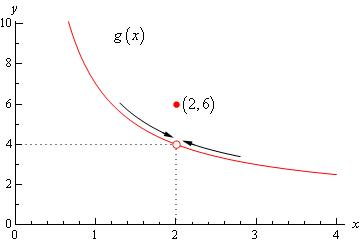
\includegraphics[width=0.5\textwidth]{oslimit2}
\end{center}
Although the \textit{value} of the function at 2 is 6, the \textit{limit} $ \lim_{x \to 6} g(x) = 4 $ because when
taking a limit we don't care what the function does at the point --- only what it looks like it should do! Essentially, the
limit of a function at a point is a property of the area around the point \textbf{and not a property of the point itself}.

\begin{ex}
  Here are a few algebraic examples:
  \begin{itemize}
    \item $ \lim_{x \to 0} \frac{x}{x} = 1 $ since as $ x $ gets closer and closer to $ 0 $, $ \frac{x}{x} = 1 $.
    \item $ \lim_{x \to 3} \frac{(x - 2)(x - 3)}{x - 3} = 1 $ since as $ x $ gets closer and closer to 3, the fraction gets arbitrarily close to 1.
    \item $ \lim_{x \to 0} \frac{1}{x} $ does not exist, since if we approach 0 from the left the function becomes arbitrarily negative
          and if we approach 0 from the right the function becomes arbitrarily positive --- we do not approach the same value on both sides.
    \item $ \lim_{x \to \infty} \frac{1}{x} = 0 $ since as $ x $ becomes arbitrarily large, $ \frac{1}{x} $ becomes arbitrarily small.
    \item $ \lim_{x \to 0} \sqrt{x} $ does not exist, since $ \sqrt{x} $ is undefined for $ x < 0 $.
  \end{itemize}
\end{ex}

Now, let's revisit the derivative. We will define the derivative of a function $ f $ at a point $ a $ as
the value of the limit
\begin{displaymath}
  \lim_{h \to 0} \frac{f(a + h) - f(a)}{h},
\end{displaymath}
which is equivalent to the definition above (see exercises).

\begin{ex}
  We will find the derivative of $ f(x) = x^3 $ at the point $ x $ using the definition.
  \begin{align*}
    f'(x) &= \lim_{h \to 0} \frac{f(x + h) - f(x)}{h}\\
          &= \lim_{h \to 0} \frac{(x + h)^3 - x^3}{h}\\
          &= \lim_{h \to 0} \frac{x^3 + 3x^2h + 3xh^2 + h^3 - x^3}{h}\\
          &= \lim_{h \to 0} \frac{3x^2 h + 3xh^2 + h^3}{h}\\
          &= \lim_{h \to 0} 3x^2 + 3xh + h^2\\
          &= 3x^2.
  \end{align*}
\end{ex}

\subsection*{Questions}
\begin{questions}
  \questioA Guess the value of the following limit by evaluating it at $ x \in \{ \pm 1, \pm 0.5, \pm 0.2, \pm 0.1, \pm 0.05, \pm 0.01 \} $:
            \begin{displaymath}
              \lim_{x \to 0} \frac{\sin x}{x + \tan x}
            \end{displaymath}
  \questioA Consider the function $ f $ graphed below.
    \begin{center}
      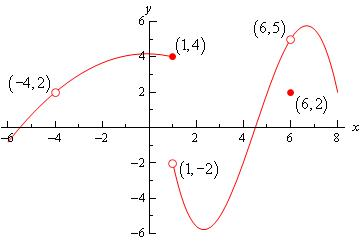
\includegraphics[width=0.4\textwidth]{oslimit}
    \end{center}
    \begin{parts}
      \part For each of the following expressions, either give the value or explain why the expression is undefined.
        \begin{subparts}
          \subpart $ f(-4) $
          \subpart $ \lim_{x \to -4} f(x) $
          \subpart $ f(1) $
          \subpart $ \lim_{x \to 1} f(x) $
        \end{subparts}
      \part Explain why the limit $ \lim_{x \to 6} f(x) $ is not equal to $ f(6) $.
      \part At which points is $ f $:
        \begin{subparts}
          \subpart Discontinuous?
          \subpart Non-differentiable?
        \end{subparts}
    \end{parts}
  \clearpage
  \questioM Evaluate the limit or explain why it does not exist:
    \begin{multicols}{2}
    \begin{parts}
      \part $ \lim_{x \to 2} \frac{x^2 + x - 6}{x - 2} $
      \part $ \lim_{x \to 0} \frac{1}{x^3} $
      \part $ \lim_{x \to 9} \frac{1}{x^3} $
      \part $ \lim_{h \to 0} \frac{(2 + h)^3 - 8}{h} $
      \part $ \lim_{x \to 4} \frac{x^2 + 5x + 4}{x^2 + 3x - 4} $
      \part $ \lim_{x \to \frac{\pi}{2}} \sin x $
      \part $ \lim_{x \to \infty} \sin x $
      \part $ \lim_{x \to \frac{\pi}{2}} \tan x $
      \part $ \lim_{x \to 0} \tan x $
      \part $ \lim_{x \to 0} \csc x $
      \part $ \lim_{x \to a} C $, where $ a $ and $ C $ are constants.
      \part $ \lim_{x \to -\infty} \tan^{-1} x $
      \part $ \lim_{y \to 0} \lim_{x \to 0} \frac{(x + y)(x - y)}{x^2 - y^2} $
      \part $ \lim_{x \to \infty} 1/x $.
      \part $ \lim_{x \to \infty} \frac{2x}{x^2 + 1} $.
      \part $ \lim_{x \to \infty} \frac{x + 2}{x - 3} $.
    \end{parts}
    \end{multicols}
  \questioM Consider the function $ \varphi $ defined by
            \begin{displaymath}
              \varphi(x) = 1/\frac{1}{x - x}.
            \end{displaymath}
            Explain why neither $ \varphi(\alpha) $ nor $ \lim_{x \to \alpha} \varphi(x) $ exists for any real $\alpha $.
  \questioM Find the derivative of $ x^2 + x $ from first principles.
  \questioE Find the derivative of $ \sin x $ from first principles, given that $ \lim_{x \to 0} \frac{\sin x}{x} = 1 $
            and $ \lim_{x \to 0} \frac{1 - \cos x}{x} = 0 $.
  \questioE Show that $ f(x) = \abs{x - 6} $ is not differentiable at $ x = 6 $. Find a formula for $ f' $.
  \questioE Show that $ \lim_{x \to a} \frac{f(x) - f(a)}{x - a} $ and $ \lim_{h \to 0} \frac{f(a + h) - f(a)}{h} $ are
            equivalent definitions for the derivative at the point $ a $ of some function $ f $.
  \questioE If $ \lim_{x \to a} [f(x) + g(x)] = 2 $ and $ \lim_{x \to a} [f(x) - g(x)] = 1 $, find $ \lim_{x \to a} f(x)g(x) $.
  \questioS Consider the following limit (you may assume that it exists):
            \begin{displaymath}
              L = \lim_{n \to \infty} \sum^n_{i = 0} \frac{9}{10^i}
            \end{displaymath}
    \begin{parts}
      \part Write $ L = 0.9 + 0.09 + \cdots $, and make a conjecture about the value of $ L $.
      \part Prove or disprove your conjecture from (a). [\textit{Hint: you may wish to consider the following working.}]
        \begin{displaymath}
          \left(1 - \frac{1}{10}\right)L = 9\left(1 - \frac{1}{10}\right)\left(\frac{1}{10} + \frac{1}{100} + \cdots\right)
        \end{displaymath}
      \part In general, consider the sum $ S_n = \sum_{i = 1}^n ar^i $ for some real constants $ a $ and $ r $. Prove that
        \begin{displaymath}
          \lim_{n \to \infty} S_n = \frac{a(1 - r^n)}{1 - r}.
        \end{displaymath}
        [\textit{Hint: use the same trick as in (b).}] Is there any restriction on $ r $ for this limit to exist?
    \end{parts}
  \clearpage
  \questioS Zeno was a Greek philosopher active in the 5th century BCE. He presented a list of `paradoxes', or apparent contradictions,
            including the following (adapted from Wikipedia):
            \begin{itemize}
              \item Suppose Achilles is in a foot race with a tortoise. Achilles runs much faster than the tortoise, but the latter
                    has a head start. By the time Achilles reaches the location that the tortoise started, the tortoise will have moved
                    a small amount further on; similarly, by the time Achilles reaches the new location of the tortoise, it will have moved
                    an even smaller distance further on; and by this reasoning it follows that Achilles can never overtake the tortoise.
                    \begin{center}
                      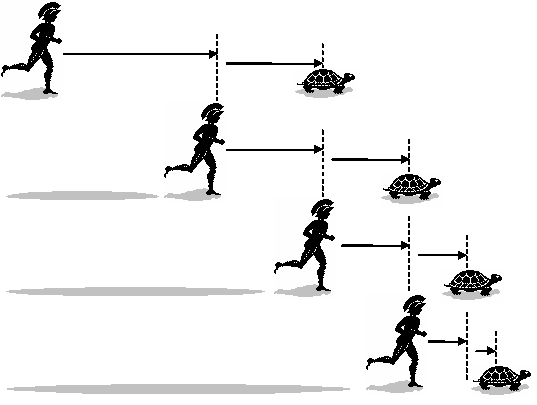
\includegraphics[width=0.4\textwidth]{achilles}
                    \end{center}
              \item Suppose Homer wishes to walk to the end of a path. Before he can get there, he must get halfway there. Before he can
                    get halfway there, he must get a quarter of the way there. Before traveling a quarter, he must travel one-eighth; before
                    an eighth, one-sixteenth; and so on. So Homer cannot walk to the end of the path.
              \item For motion to occur, an object must change the position which it occupies. Consider an example of an arrow in flight. In any
                    one (duration-less) instant of time, the arrow is neither moving to where it is, nor to where it is not. It cannot move to
                    where it is not, because no time elapses for it to move there; it cannot move to where it is, because it is already there.
                    In other words, at every instant of time there is no motion occurring. If everything is motionless at every instant, and
                    time is entirely composed of instants, then motion is impossible.
            \end{itemize}
            Use your knowledge of limits to explain these apparent contradictions.
\end{questions}
\end{document}

\section{Taking derivatives}
Taking derivatives using the definitions quickly becomes unmanagable. Because of this,
we want to produce a set of rules which will allow us to take derivatives of common
functions.

\subsection{Differentiation of polynomials}
We begin with a few easy observations that will allow us to take derivatives of
polynomials.

\begin{thm}[Arithmetic of derivatives]
  Let $ f $ and $ g $ be functions.
  \begin{enumerate}
    \item If $ f(x) = \lambda $ for all $ x $ (where $ \lambda $ is a constant), then $ f'(x) = 0 $ for all $ x $.
    \item The derivative of $ f + g $ is $ f' + g' $ (i.e. for all $ x $, $ (f + g)'(x) = f'(x) + g'(x) $).
    \item If $ \lambda $ is a constant, then $ (\lambda f)' = \lambda f' $.
  \end{enumerate}
\end{thm}
\begin{proof}
  \begin{enumerate}
    \item In this case, $ \frac{f(x + h) - f(x)}{h} = \frac{\lambda - \lambda}{h} = 0 $, so the difference quotient is always zero and so is the derivative.
    \item If $ h $ is small, $ (f + g)(x + h) - (f + g)(x) =  f(x + h) + g(x + h) - f(x) - g(x) \approx f'(x)h + g'(x)h $ and so the derivative at $ x $
          is $ f'(x) + g'(x) $.
    \item $ (\lambda f)(x + h) - (\lambda f)(x) = \lambda (f(x + h) - f(x)) \approx \lambda (f'(x) h) = (\lambda f')(x) h $.
  \end{enumerate}
\end{proof}

Now we consider $ f(x) = x^n $ for integers $ n $. Using the binomial theorem,
\begin{displaymath}
  \lim_{h \to 0} \frac{f(x + h) - f(x)}{h} = \lim_{h \to 0} \frac{(x + h)^n - x^n}{h} = \lim_{h \to 0} \frac{x^n + n x^{n - 1} h + \cdots - x^n}{h}
\end{displaymath}
where every term hidden in the $ \cdots $ includes an $ h^2 $ factor, so we obtain
\begin{equation}
  f'(x) = \lim_{h \to 0} n x^{n - 1} + h(\cdots) = nx^{n - 1}.
\end{equation}
In fact, although we proved this for integer $ n $, it holds in general:
\begin{thm}[Power law]
  If $ f(x) = x^\alpha $ then $ f'(x) = \alpha x^{\alpha - 1} $.
\end{thm}

\begin{ex}
  We can now differentiate every function of the form $ f(x) = a_1 x^{b_1} + \cdots + a_n x^{b_n} $: $ f'(x) = b_1 a_1 x^{b_1 - 1} + \cdots + b_n a_n x^{b_n - 1} $.
  In particular, if $ f(x) = \sqrt{x} $ then $ f'(x) = \frac{1}{2\sqrt{x}} $; if $ g(x) = 2x^2 + 3 $ then $ g'(x) = 4x $; and if $ h(x) = \frac{1}{x} + x^7 $
  then $ h'(x) = -\frac{1}{x^2} + 7x^6 $.
\end{ex}

\subsection{Trigonometric derivatives}
We have already seen that $ \sin' = \cos $; using similar reasoning, we can prove the following:

\begin{thm}[Trigonometric derivatives]
  \def\arraystretch{1.5}
  \begin{tabular}{|c|c|l|}\hline
    \textbf{Function} & \textbf{Derivative} \\\hline
    $ \sin x $ & $ \cos x $\\\hline
    $ \cos x $ & $ -\sin x $\\\hline
    $ \tan x $ & $ \sec^2 x $\\\hline
    $ \csc x $ & $ -\csc x \cot x $\\\hline
    $ \sec x $ & $ \sec x \tan x $\\\hline
    $ \cot x $ & $ -\csc^2 x $\\\hline
  \end{tabular}
\end{thm}

I will use the result $ \sin' = \cos $ to prove that $ \cos' = -\sin $, and we will prove
the rest at a later time. Indeed, $ \cos x = \sin (x + \pi/2) $; then $ \od{}{x} \cos x = \od{}{x} \sin(x + \pi/2) $.
But the graph of $ \sin(x + \pi/2) $ is just the graph of $ \sin x $, shifted to the left
by $ \pi/2 $. Hence the slope of $ \sin (x + \pi/2) $ is the same as the slope of $ \sin x $,
but shifted to the left by $ \pi/2 $; and the slope of $ \sin x $ is $ \cos x $. Hence:
\begin{equation}
  \od{}{x} \cos x = \od{}{x} \sin(x + \pi/2) = \cos(x + \pi/2) = -\sin x.
\end{equation}
(This little trick I used here is explored in more detail in the L2 notes; we don't need it
too often this year, because in a couple of sections we will learn a much more general way
of dealing with this kind of situation.)

\begin{app}
  Many phenomena in physics can be modelled with sine waves; for example, if a particle on the end of a spring
  is moving with simple harmonic motion, then it has position $ x = A \sin (\omega t + \phi) $; taking derivatives,
  we find that it has velocity $ v = \od{x}{t} = A\omega \cos (\omega t + \phi) $ and acceleration $ a = \od[2]{x}{t} = -A \omega^2 \sin (\omega t + \phi) $.
  In other words, it is always accelerating in the opposite direction to its movement!
\end{app}

\subsection{Exponential functions}
The next function we want to consider here is $ f(x) = a^x $, for constants $ a $. We can
compute that
\begin{displaymath}
  f'(x) = \lim{h \to 0} \frac{a^{x + h} - a^x}{h} =  a^x \lim_{h \to 0} \left( \frac{a^h - 1}{h} \right).
\end{displaymath}
So the exponential functions $ a^x $ have derivatives of the form $ Ka^x $, where $ K $ is some constant. This
begs the question, for which value of $ a $ (if any) does $ \od{}{x} a^x = a^x $ (i.e. $ K = 1 $)? Well, we
need to solve
\begin{displaymath}
  \lim_{h \to 0} \left( \frac{a^h - 1}{h} \right) = 1
\end{displaymath}
for $ a $. We will begin by setting $ u = 1/h $, so when $ h \to 0 $ we have $ u \to \infty $. Thus
\begin{displaymath}
  \lim_{u \to \infty} (a^{1/u} - 1)u = 1 = \lim_{u \to \infty} 1;
\end{displaymath}
and applying the limit laws,
\begin{align*}
  \lim_{u \to \infty} (a^{1/u} - 1) &= \lim_{u \to \infty} \frac{1}{u};\\
  \lim_{u \to \infty} a^{1/u} &= \lim_{u \to \infty} \frac{1}{u} + 1;\\
  a = \lim_{u \to \infty} (a^{1/u})^u &= \lim_{u \to \infty} \left(\frac{1}{u} + 1\right)^u.
\end{align*}
It can be shown fairly easily that $ \lim_{u \to \infty} \left(\frac{1}{u} + 1\right)^u $ does
indeed exist (it has a value of $ 2.71828... $), and we define its value to be $ e $. Thus $ e $
is the base for the exponential function that is its own derivative: $ \od{}{x} e^x = e^x $. Often,
we write $ \exp(x) := e^x $.

Finally, note that if $ K = \lim_{h \to 0} \left( \frac{a^h - 1}{h} \right) = \lim_{u \to \infty} u(a^{1/u} - 1) $ then
\begin{displaymath}
  a = \lim_{u \to \infty} \left(\frac{K}{u} + 1\right)^u = \lim_{u \to \infty} \left(\left(\frac{K}{u} + 1\right)^{u/K}\right)^K = \lim_{(u/K) \to \infty} \left(\left(\frac{K}{u} + 1\right)^{u/K}\right)^K = e^K;
\end{displaymath}
hence $ \od{}{x} a^x = a^x K = a^x \log_e a $. (We normally write $ \log_e = \ln $.)

\subsection{Logarithmic derivatives}
Finally, let us calculate $ \od{}{x} \ln x $. (This will allow us to find $ \od{}{x} \log_a x $ for all $ a $, using the
relationship $ \log_a x = \frac{1}{\ln a} \ln x $.)

\begin{displaymath}
  \ln'(x) = \lim_{h \to 0} \frac{\ln(x + h) - \ln(x)}{h} = \lim_{h \to 0} \frac{1}{h} \ln\left(1 - \frac{h}{x} \right) = \lim_{h \to 0} \ln\left(1 - \frac{h}{x} \right)^{1/h}
\end{displaymath}
Let $ u = 1/h $; so as $ h \to 0 $, $ u \to \infty $. Then, substituting, we obtain
\begin{displaymath}
  \ln'(x) = \lim_{u \to \infty} \ln \left( 1 - \frac{1}{ux} \right)^u.
\end{displaymath}
Now, we use the fact that $ \exp(\ln x) = x $:
\begin{displaymath}
  e^{\ln'(x)} = \lim_{u \to \infty} \exp(\ln \left( 1 - \frac{1}{ux} \right)^u) = \lim_{u \to \infty}\left( 1 - \frac{1}{ux} \right)^u
              = \lim_{u \to \infty} \left(\left( 1 - \frac{1}{ux} \right)^{ux}\right)^{(1/x)}
              = e^{1/x}
\end{displaymath}
and thus $ \ln'(x) = 1/x $.

\subsection{Exercises and Problems}
\begin{enumerate}
  \item Find the derivatives of $ 3x^3 $, $ 2x^2 $, and $ 6x^5 $. Conclude that $ (fg)' \neq f' g' $ in general.
  \item Find the derivatives of the following functions with respect to $ t $:
    \begin{enumerate}
      \item $ y = 2t^3 + 3t^2 $
      \item $ y = \sqrt{t} $
      \item $ y = (2t + 1)(t - 4) $
      \item $ g(t) = 4 \sec t + 9 \tan t $
      \item $ h(t) = \sqrt[5]{t} + 2\csc t - \ln t^3 $
      \item $ \phi'(t) = \csc x + 12x^{1273} + 9 $
      \item $ y = 2017t^{2016} + (t + 2)^2 $
      \item $ y = 940\sin t + \frac{1}{2}e^{t + 2} $
    \end{enumerate}
  \item Where is the function $ x \mapsto x^3 - 2x^2 - x + 1 $ increasing?
  \item Find the velocity $ v $ of a particle at time $ t = 2\pi $ if its position function for $ t > 0 $ is $ x = e^t - \sin t $.
  \item Find the slope of the tangent line to $ y = x + \tan x $ at $ (\pi, \pi) $.
  \item Find a linear approximation $ \tilde f $ to $ f(x) = x^2 + x + 1 $ at $ (0,1) $, and find some $ \delta $ such
        that for all $ x $ satisfying $ -\delta < x < \delta $, $ -0.1 < \tilde f(x) - f(x) < 0.1 $.
  \item It is \textbf{not} true that the derivative of $ f(g(x)) $ is $ f'(g'(x)) $.
    \begin{enumerate}
      \item For a counterexample, consider $ f(x) = x^2 $ and $ g(x) = x $; show that $ f'(g'(x)) = 2 $, but $ \od{}{x} f(g(x)) = 2x $.
      \item Compute the derivative of $ \ln x^2 $.
    \end{enumerate}
  \item Suppose the derivative of a function is $ \od{y}{x} = 3x^2 - x - 4 $. What could the original function be?
  \item Find the 64th derivative of $ \sin x $.
  \item Find the $ n$th derivative of $ x^n $.
  \item If $ y = 2\sin 3x \cos 2x $, find $ \od{y}{x} $. (Hint: use an identity to rewrite this as a sum of functions.)
  \item For which values of $ x $ does the graph of $ f(x) = x + 2\sin x $ have a horizontal tangent?
  \item Show that $ y = 6x^3 + 5x - 3 $ has no tangent line with a slope of 4.
  \item Find real values of $ \alpha $ and $ \beta $ such that, if $ y = \alpha \sin x + \beta \cos x $,
        then $ y'' + y' -2y = \sin x $.
  \item Consider a \SI{12}{\metre} long ladder leaning against a wall such that the top of the ladder makes an
        angle $ \theta $ with the wall. If this angle $ \theta $ is varied, the distance $ D $ between the bottom
        of the ladder and the wall also changes. If $ \theta = \pi/3 $, what is the rate of change of $ D $ with
        respect to $ \theta $?
  \item Prove that the function $ \varphi $ given by $ \varphi(x) = \frac{x^{101}}{101} + \frac{x^{51}}{51} + x + 1 $
        never has a horizontal tangent line.
  \item The derivative is primarily a geometric concept, not an algebraic one.
    \begin{enumerate}
      \item The area of a circle of radius $ r $ is $ A = \pi r^2 $. Find $ \od{A}{r} $. What do you notice?
      \item Explain item (a) geometrically.
      \item The volume of a sphere is given by $ V = \frac{4}{3} \pi r^3 $. Find an expression for the surface area.
    \end{enumerate}
\end{enumerate}

\subsection{References}
See sections 2.1 -- 2.4 of Stewart. For a discussion of the exponential function and its
relationship to compound interest and rates of growth, see Thompson chapter XIV.

\subsection{Homework problems}
\begin{enumerate}
  \item Differentiate with respect to $ x $:
    \begin{enumerate}
      \item $ x^2 + \frac{1}{x} $
      \item $ tx^t $
      \item $ \sin x - \cos x $
      \item $ \sqrt[5]{x^4} $
    \end{enumerate}
  \item Explain why you cannot use the power rule to find the derivative of $ x^x $.
  \item Find the $ n$th derivative of $ \frac{1}{x^n} $.
  \item Suppose a population grows exponentially with time, such that after $ t $ years the population is $ P(t) = P_0 + 10^t $.
    \begin{enumerate}
      \item Find the rate of change of the population at $ t = 100 $.
      \item Explain why this population model is unrealistic.
    \end{enumerate}
\end{enumerate}

\section{Anti-derivatives}
We now want to begin to study the inverse of differentiation: the problem is, given
a function $ f $, to find some function $ F $ which has $ f $ as a derivative. Geometrically,
we are given the rate of change of a function at every point, and we wish to recover the
original function.

If $ f = F' $, then $ F $ is said to be an \emph{anti-derivative} of $ f $.

First of all, we notice that if $ F $ is an anti-derivative of $ f $ then so is $ F + C $
for any constant $ C $; this is because $ (F + C)' = F' + C' = F' + 0 = F' = f $. Thus
when we take anti-derivatives there are infinitely many different solutions that all differ
by a constant --- we cannot recover the original function given a slope function without
some more information. These functions are said to be the family of solutions that solve the
differential equation $ F' = f $; we will also write $ F(x) + C = \rint f(x) \dif{x} $ in
this case, and we say that $ F $ is the \emph{indefinite integral} of $ f $; in the
expression $ \rint f(x) \dif{x} $, $ f(x) $ is called the \emph{integrand}.

The reason for this terminology comes from the geometric meaning of the derivative --- if
$ F $ is an anti-derivative of $ f $, then $ f $ is the slope function of $ F $. This in
turn means that each value of $ f $ tells us how quickly $ F $ is rising or falling at that
point; roughly speaking, to get $ F $ back from $ f $, we need to walk along $ f $, adding
up all these infinitesimal rises and falls of $ F $ --- in other words, we need to take
all the values of $ f $, and `integrate' (combine) them together to get back the form of $ F $.

This idea is made precise in the \emph{fundamental theorem of calculus}, which we will state later on. This
same theorem tells us that if $ f $ is a continuous function then there exists some anti-derivative $ F $
of $ f $, and that this anti-derivative is unique up to a constant.

\begin{center}
  \def\arraystretch{2}
  \begin{tabular}{|c|c|c|}\hline
    \textbf{Differential equation} && \textbf{Integral equation}\\\hline
    $ f $ is the slope function of $ F $ & $\displaystyle\iff$ & $ F $ is an anti-derivative of $ f $ \\\hline
    $\displaystyle f(x) = F'(x) $ &$\displaystyle\iff$& $\displaystyle F(x) + C = \rint f(x) \dif{x} $\\\hline
    $\displaystyle f(x) = \dod{y}{x} $ &$\displaystyle\iff$& $\displaystyle y + C = \rint f(x) \dif{x} $\\\hline
  \end{tabular}
\end{center}

There are a few simple rules that we can state right away. For example, we have the following power
rule for differentiation:
\begin{displaymath}
  \od{}{x} ax^n = nax^{n - 1} \iff \rint nax^{n - 1} \dif{x} = ax^n + C
\end{displaymath}
so the anti-derivatives of $ ax^n $ are $ \frac{a}{n + 1} x^{n + 1} + C $.

Looking at the inverse power law, we notice that there is an issue when we try to anti-differentiate
$ 1/x $; the law tells us that $ \rint x^{-1} \dif{x} = \frac{1}{1 - 1} x^{0} $, which is plainly nonsense. Luckily,
last week we showed that $ \od{}{x} \ln x = 1/x $, so $ \rint 1/x \dif{x} = \ln x + C $.

Some more useful rules come by way of our differentiation arithmetic laws.
\begin{thm}
  \begin{enumerate}
    \item $ \rint 0 \dif{x} = C $ (the family of constant functions)
    \item $ \rint f(x) + g(x) \dif{x} = \rint f(x) \dif{x} + \rint g(x) \dif{x} $
    \item $ \rint \lambda f(x) \dif{x} = \lambda \rint f(x) \dif{x} $
  \end{enumerate}
\end{thm}
\begin{proof}
  \begin{enumerate}
    \item Firstly, $ \od{}{x} 0 = 0 $; so the anti-derivatives of $ 0 $ are $ 0 + C = C $.
    \item Let $ F $ and $ G $ be anti-derivatives of $ f $ and $ g $, so $ F' = f $ and $ G' = g $.
          Then $ \rint f(x) \dif{x} + \rint g(x) \dif{x} = F(x) + G(x) + C $ (*); but $ \od{}{x} [F(x) + G(x) + C] = f(x) + g(x) $
          and so $ F + G + C $ is an anti-derivative of $ f + g $ and $ \rint f(x) + g(x) \dif{x} = F(x) + G(x) + C $. Combining
          this with (*) we obtain the result.
    \item Let $ F $ be an anti-derivative of $ f $. Then $ (\lambda F)' = \lambda (F') = \lambda f $, and thus $ \lambda F $ is
          an anti-derivative of $ \lambda f $; so $ \rint \lambda f(x) \dif{x} = \lambda F(x) = \lambda \rint f(x) \dif{x} $.
  \end{enumerate}
\end{proof}

\begin{ex}
  One anti-derivative of $ y' = 3x^2 + 4 $ is $ x^3 + 4x $. Another is $ x^3 + 4x + 1 $. A third is $ x^3 + 4x + 7 $.
\end{ex}

Unfortunately, there is no `easy' way to anti-differentiate; we simply have to try to rearrange the function in some clever
way until it looks like something that we know how to deal with.

\begin{exs}\leavevmode
  \begin{enumerate}
    \item The most general antiderivative of $ \sin x $ is $ -\cos x + C $.
    \item The most general antiderivative of $ \tan x $ is $ -\ln \abs{\cos x} + C $.
    \item $ \rint \frac{1}{x + 3} \dif{x} = \ln \abs{x + 3} + C $.
    \item $ \rint \tan^2 \theta \dif{\theta} = \rint \sec^2 \theta - 1 \dif{\theta} = \tan \theta - \theta + C $.
    \item $ \rint \frac{2x}{x^2 + 1} \dif{x} = \ln \abs{x^2 + 1} + C $.
    \item $ \rint Ke^{Kx} \dif{x} = e^{Kx} + C $ for all constants $ K $.
  \end{enumerate}
\end{exs}

\begin{joke}
  Two mathematicians are in a bar. The first one says to the second that the average person knows very little about basic
  mathematics. The second one disagrees and claims that most people can cope with a reasonable amount of maths. The first
  mathematician goes off to the washroom, and in her absence the second calls over the waiter. She tells the waiter that in a few
  minutes, after her friend has returned, she will call him over and ask him a question. All he has to do is answer ``one
  third $x$ cubed.'' He repeats ``one thir-dex cue?'' She repeats ``one third $x$ cubed.'' He asks, ``one thir dex cuebd?'' ``Yes,
  that’s right,'' she says. So he agrees, and goes off mumbling to himself, ``one thir dex cuebd...''. The first mathematician returns
  and the second proposes asking the waiter for an anti-derivative to prove her point that most people do know something about basic maths;
  the first laughingly agrees. The second mathematician calls over the waiter and asks ``what is the integral of $x$ squared?'' The waiter
  says ``one third $x$ cubed'' and while walking away, turns back and says over his shoulder, ``plus a constant!''
\end{joke}

\subsection{Inverse problems (optional)}
In mathematics there are a lot of examples of operations which are easy to perform
in one direction, but harder to reverse.

\begin{center}
  \begin{tabular}{c|c}
    \textbf{Easy} & \textbf{Hard}\\
    addition & subtraction\\
    multiplication & division\\
    expanding & factorising\\
    exponents & logarithms\\
    tying a knot & unravelling a knot\\
    differentiation & anti-differentiation
  \end{tabular}
\end{center}

One very important application of this idea is in cryptography. Most modern computer
systems are dependent on something known as the RSA cipher, which essentially relies
on the fact that it's much easier to multiply large primes together than it is to
work out what primes divide a large integer.

Anti-differentiation in particular is very difficult, in the sense that there are
rules that enable us to take the derivative of every combination of `simple' functions
(polynomials, exponentials, logarithms, trig functions, sums, products, functions of
functions) --- but there are some functions, made up of these building blocks, which
do not have anti-derivatives of the same type.

For example, there is no anti-derivative of $ x^x $ which can be produced with simple
functions. There is a function $ f $ such that $ f'(x) = x^x $, we just can't write it
down at all using any combination of these building blocks despite the function $ x \mapsto x^x $
being made up of them.

\subsection{Exercises and Problems}
\begin{enumerate}
  \item For each expression, find the most general anti-derivative with respect to $ x $.
    \begin{multicols}{2}
    \begin{enumerate}
      \item $ 2x $
      \item $ x^2 + 3x + 1 $
      \item $ \frac{1}{2\sqrt{x}} $
      \item $ x^{-3} $
      \item $ 10^x $
      \item $ \sec^2 x + \sqrt{x} $
      \item $ x\sqrt{x} $
      \item $ \sin x - \cos x $
      \item $ \frac{2x^3 + 3x - \sqrt{x}}{\sqrt[3]{x}} $
      \item $ \frac{1}{x^2} + e^x $
      \item $ \sec^2 (x + 1) $
    \end{enumerate}
    \end{multicols}
  \item Verify the examples in the notes by differentiation.
  \item Show that $ \rint 3x^2 + 4x + 5 + \frac{2}{x} \dif{x} = x^3 + 2x^2 + 5x + \ln x^2 + C $.
  \item If $ \od{y}{t} = 1.5 \sqrt{t} $ and $ y(4) = 10 $, find $ y(t) $ exactly.
  \item Find $ f $ if $ f''(x) = 12x^2 + 6x - 4 $, $ f(0) = 4 $, $ f(1) = 1 $.
  \item The velocity of a particle is given by $ v(t) = 2t + 1 $. Find its position at $ t = 4 $
        if its position at $ t = 0 $ is $ x = 0 $.
  \item The acceleration of a particle is given by $ a(t) = 10\sin t + 3\cos t $. At $ t = 0 $, its position is $ x = 0 $; at $ t = 2\pi $,
        its position is $ x = 12 $. Find its position at $ t = \frac{\pi}{2} $.
  \item Starting from rest, a car takes $ T $ seconds to reach its maximum speed, $ v_\text{max} $. A plausible
        model for the velocity of the car after $ t $ seconds is
        \begin{displaymath}
          v(t) = \begin{cases} v_\text{max} \left( \frac{2t}{T} - \frac{t^2}{T^2} \right) & t \leq T, \\ v_\text{max} & t \geq T. \end{cases}
        \end{displaymath}
    \begin{enumerate}
      \item Write an expression for $ a_\text{max} $, the maximum acceleration attained by the car.
      \item Show that the distance travelled by the car from the time it starts to the point it reaches its maximum
            speed is given by $ s(t) = \frac{1}{3} a_\text{max} T^2 $.
    \end{enumerate}
  \item Find all functions $ g $ such that $ g'(x) = 4 \sin x + \frac{2x^5 - \sqrt{x}}{x} $.
  \item For each function, sketch an anti-derivative passing through $ (0, 0) $:
        \begin{center}
          \begin{tabular}{ccc}
            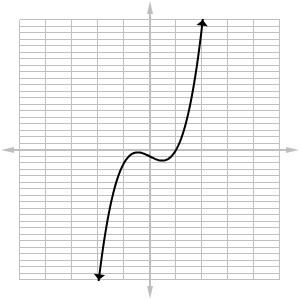
\includegraphics[width=0.28\textwidth]{anti1}&
            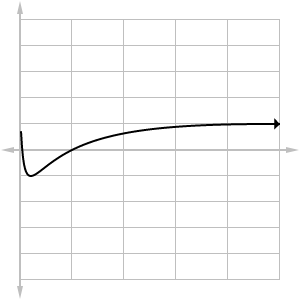
\includegraphics[width=0.28\textwidth]{anti2}&
            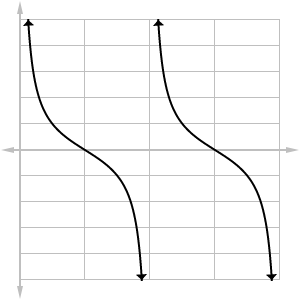
\includegraphics[width=0.28\textwidth]{anti3}\\
            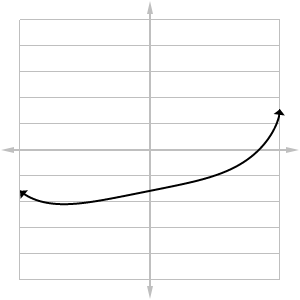
\includegraphics[width=0.28\textwidth]{anti4}&
            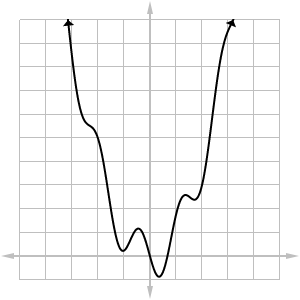
\includegraphics[width=0.28\textwidth]{anti5}&
            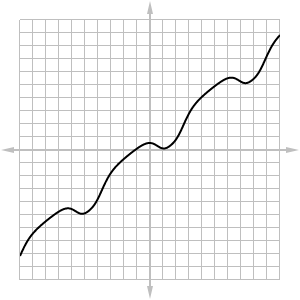
\includegraphics[width=0.28\textwidth]{anti6}
          \end{tabular}
        \end{center}
  \item Show that if $ F $ is an anti-derivative of $ f $, $ G $ is an anti-derivative of $ g $, and $ \alpha $ and $ \beta $ are any constants,
        then $ \alpha F + \beta G $ is an anti-derivative of $ \alpha f + \beta g $.
  \item Give an example of functions $ f $ and $ g $ such that if $ F $ and $ G $ are anti-derivatives of $ f $ and $ g $ respectively then $ FG $
        is \emph{not} an anti-derivative of $ fg $.
\end{enumerate}

\subsection{References}
Because of the way we're covering integration, most books will have problems which we can't
do yet (for example, $ \rint \tan x \dif{x} $). That said, many more anti-differentiation problems
can be found in the following: Stewart, section 4.4; Thompson, chapter XVIII.

\subsection{Homework problems}
\begin{enumerate}
  \item Find the most general anti-derivative.
    \begin{enumerate}
      \item $ f(x) = x - 3 $
      \item $ f(x) = (x + 1)(x + 2) $
      \item $ f(\theta) = 6\theta^2 - 7 \sec^2 \theta $
      \item $ g(h) = \pi^2 $
      \item $ f(x) = x^{3.7} + \sqrt{x} + 7x^{\sqrt{7} - 1} $
    \end{enumerate}
  \item Given that the graph of $ \varphi $ passes through the point $ (1, 6) $
        and that the slope of its tangent line at $ (x, \varphi(x)) $ is $ 2x + 1 $,
        find $ \varphi(2) $.
  \item This is the second derivative of $ g $. Find $ g $ given that $ g'(0) = 0 $ and $ g(0) = 1 $.
        \begin{center}
          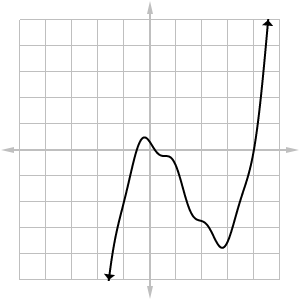
\includegraphics[width=0.4\textwidth]{anti7}
        \end{center}
\end{enumerate}

\section{The chain rule}
\begin{figure}
  \centering
  \begin{tikzpicture}
    \begin{axis}[
        axis lines = none,
        scale = 1.5,
        xmin = -7,
        x = 0.2cm
      ]
      \addplot[color = red, domain = 0:2*pi, samples = 200] {sin(deg(x^2)) + 4.5};
      \addplot[color = blue, domain = 0:4*pi^2, samples = 100] {sin(deg(x))};
      \draw[<->] (0, 2) -- (4*pi^2, 2);
      \draw[<->] (0, 3) -- (2*pi, 3);
      \draw (-1.25,2) node[left] {$ u = x^2 $};
      \draw (-1.25,3) node[left] {$ x $};
      \draw (-1.25,0) node[left] {$ \sin u $};
      \draw (-1.25,4.5) node[left] {$ \sin x^2 $};

      \draw[color = gray, style=dotted] (0, 2)      -- (0,3);
      \draw[color = gray, style=dotted] (2.46, 2)   -- (1.57,3);
      \draw[color = gray, style=dotted] (9.86, 2)   -- (3.14,3);
      \draw[color = gray, style=dotted] (22.21, 2)  -- (4.71,3);
      \draw[color = gray, style=dotted] (4*pi^2, 2) -- (2*pi,3);
    \end{axis}
  \end{tikzpicture}
  \caption{A graphic showing how the change of variables $ u \leftrightarrow x^2 $ stretches the graph of $ \sin $.}
\end{figure}

Consider the function $ x \mapsto \sin (x^2) $. This function is made up of two
functions, applied one after the other:
\begin{displaymath}
  x \xmapsto{f} x^2 \xmapsto{g} \sin(x^2).
\end{displaymath}
We often notate this function composition as $ g \circ f $ (note that we
evaluate from the right, so $ (g \circ f)(x) = g(f(x)) $).

Obviously the derivative of $ \sin(x^2) $ is not just $ \cos(2x) $, since the former
has a horizontal tangent line at $ x = \sqrt{\dfrac{\pi}{2}} $ but $ \cos(\sqrt{2\pi}) \neq 0 $. This
shows us that, in general, the derivative of a function composition is not simply the composition
of the derivatives.

In fact, it turns out that the derivative of $ f \circ g $ is $ g' \times (f' \circ g) $; in other words,
\begin{displaymath}
  \od{}{x} f(g(x)) = g'(x) f'(g(x)).
\end{displaymath}
This is known as the \emph{chain rule}, since we are ``chaining'' together functions.

Let us convince ourselves that this rule is plausible. We can interpret the derivative $ \od{g}{x} $ as the rate of change
of $ g $ with respect to $ x $, and the derivative $ \od{f}{g} $ as the derivative of $ f $ with respect to small changes in
the output of $ g $; it is intuitive that if $ g $ changes twice as fast as $ x $ at some point, and $ f $ changes five
times as fast as $ g $, then $ f $ changes $ 2 \times 5 = 10 $ times as fast as $ x $.

The proof goes something like this: consider $ f(g(x + h)) - f(g(x)) $ for small $ h $. We want to write this as $ m h $, where $ m $
is only dependent on $ x $. Now, since $ h $ is small, $ g(x + h) \approx g(x) + g'(x)h $. Thus $ f(g(x + h)) - f(g(x)) \approx f(g(x) + g'(x)h) - f(g(x)) $.
But if $ h $ is small enough, then $ u = g'(x) h $ is small too; so, if $ y = g(x) $, then
\begin{multline*}
  f(g(x + h)) - f(g(x)) \approx f(g(x) + g'(x)h) - f(g(x))\\
    = f(y + u) - f(y) \approx f'(y)u = f'(g(x)) f'(x)h.
\end{multline*}
Thus $ (f \circ g)(x + h) - (f \circ g)(x) \approx f'(g(x)) f'(x) h $, and so $ (f \circ g)'(x) = f'(g(x)) f'(x) $.

\begin{exs}\leavevmode
  \begin{enumerate}
    \item The correct derivative of $ \sin(x^2) $ is $ 2x \cos(x^2) $.
    \item If $ f(r) = \sqrt{r^2 - 3} $, then $ f'(r) = 2r \frac{1}{2} \left(r^2 - 3\right)^{-1/2} = \dfrac{r}{\sqrt{r^2 - 3}} $.
    \item If $ g(x) = \sin((\sin^7 x^7 + 1)^7) $, then we compute:
          \begin{align*}
            g(x)  &= \sin \left( \left[ \left( \sin x^7 \right)^7 + 1 \right]^7 \right)\\
            g'(x) &= 7x^6 \cdot \cos x^7 \cdot 7\left(\sin x^7\right)^6 \cdot 7\left[\left(\sin x^7\right)^7 + 1\right]
                          \cdot \cos \left( \left[ \left( \sin x^7 \right)^7 + 1 \right]^7 \right)
          \end{align*}
  \end{enumerate}
\end{exs}

We can use the chain rule to relate rates of change together --- for example, the area of a circle is given by $ A = \pi r^2 $
and so the rate of change of area with respect to radius $ \od{A}{r} = 2\pi r $; but if $ r $ varies with respect to time then
we can find the rate of change of the area with respect to time using the chain rule.

A useful mnemonic is (if $ x $ is a function of $ y $ which is itself a function of $ z $)
\begin{equation}
  \od{x}{y} \cdot \od{y}{z} = \od{x}{z}. \tag{chain rule}
\end{equation}
We can also apply the inverse function rule for differentiation, which tells us that
\begin{equation}
  \od{x}{y} = \frac{1}{\od{y}{x}}. \tag{inverse function rule}
\end{equation}
The inverse rule is easy to prove: if $ f $ is a function, we have that $ f(f^{-1}(y)) = y $. Taking the derivative of
both sides, $ f'(f^{-1}(y)) \cdot (f^{-1})'(y) = 1 $ and therefore $ (f^{-1})'(y) = \dfrac{1}{f'(f^{-1}(y))} $.

These two operations allow us to rearrange equations as if $ \od{y}{x} $ were a fraction. There isn't much of a problem
if you do think of it in this way, as long as you're careful.

\begin{ex}[Inverse function rule]
  Let us find $ \od{}{x} \tan^{-1} x $. If $ y = \tan^{-1} x $, then $ x = \tan y $; the inverse
  function rule tells us that $ \od{y}{x} = \frac{1}{\od{x}{y}} = \frac{1}{\sec^2 y} = \cos^2 y $.
  Substituting for $ y $, $ \od{y}{x} = (\cos \tan^{-1} x)^2 = \frac{1}{x^2 + 1} $.\footnote{We proved
  that $ \cos \tan^{-1} x = \frac{1}{\sqrt{x^2 + 1}} $ in the trigonometry notes.}
\end{ex}

\begin{ex}
  A ladder \SI{5}{\metre} long rests against a vertical wall. If the bottom of the ladder slides away
  from the wall at a rate of \SI{1}{\metre\per\second}, how fast is the top of the ladder sliding down the
  wall when the bottom of the ladder is \SI{3}{\metre} from the wall?

  \textit{Solution.} Let $ x $ be the distance of the bottom of the ladder from the wall, and let $ y $
  be the height of the top of the ladder up the wall. We have $ \od{x}{t} = 1 $ and $ x = 3 $; we also
  know that $ y = \sqrt{25 - x^2} $, so:
  \begin{align*}
    \dod{y}{t} &= \dod{y}{x} \cdot \dod{x}{t} = -\frac{x}{\sqrt{25 - x^2}} \cdot 1\\
    \eval{\dod{y}{t}}_{x = 3} &= -\frac{3}{\sqrt{25 - 9}} = -\frac{3}{4}.
  \end{align*}
  Hence the ladder is sliding down the wall at a rate of \SI{-0.75}{\metre\per\second}.
\end{ex}

\begin{ex}
  The radius of a sphere is increasing at a rate of $ \od{r}{t} = -\ln(t - 1) $ metres per second. At what rate will the surface area of
  the sphere be growing at $ t = 2 $?

  \textit{Solution.} We have $ \mathrm{SA} = 4\pi r^2 $, so $ \od{\mathrm{SA}}{r} = 8\pi r $ and
    \begin{displaymath}
      \od{\mathrm{SA}}{t} = \od{\mathrm{SA}}{r} \od{r}{t} = -\ln(t - 1) \times 8\pi r = 0.
    \end{displaymath}

    The surface area of the sphere will be momentarily constant at $ t = 2 $.
\end{ex}

\subsection{Exercises and Problems}
\begin{enumerate}
  \item Identify the inner and outer functions, but don't try to differentiate.
    \begin{enumerate}
      \item $ \sqrt{\sin x} $
      \item $ \sin \cos \tan x $
      \item $ (2x + 3)^{17} $
      \item $ 97(x + 2)^2 $
      \item $ \ln \sin x $
      \item $ \frac{1}{\sqrt{23x - x^2}} $
    \end{enumerate}
  \item Differentiate with respect to $ t $:
    \begin{multicols}{2}
    \begin{enumerate}
      \item $ (2t + 3)^{3000} $
      \item $ \sin \ln t $
      \item $ \sqrt{t^3 + 10t^2 + 3} $
      \item $ \csc e^t $
      \item $ \sin^3 t + 14\ln (3t) $
      \item $ \sin \sin \sin t $
      \item $ \cot (t + \sec t) $
      \item $ \sin^2 ((t + \sin t)^2) $
      \item $ \ln \sqrt{t + 9} $
      \item $ \sqrt{t} + \frac{1}{\sqrt[3]{t^4}} $
      \item $ e^{\sec (t^2)} $
      \item $ \sin \sqrt{t + \tan t} $
    \end{enumerate}
    \end{multicols}
  \item The derivative of a function is $ 2 \cos 2x $. What could the original function be?
  \item Differentiate $ y = \sin^2 x + \cos^2 x $, and hence prove that $ \sin^2 x + \cos^2 x = 1 $.
  \item Suppose that the displacement of a particle on a vibrating spring is given by $ x(t) =  5 + \frac{1}{8} \sin(5\pi t) $,
        where $ x $ is measured in centimetres and $ t $ in seconds.
    \begin{enumerate}
      \item Find the velocity of the particle at time $ t $.
      \item At which times is the particle momentarily stationary?
    \end{enumerate}
  \item Find a linear approximation $ \tilde f $ around 0 for $ f(x) = \sqrt[4]{1 + 2x} $; then calculate $ \delta $ such that
        for all $ x $ satisfying $ -\delta < h < \delta $, $ -0.1 < \tilde f(x) - f(x) < 0.1 $.
  \item The volume of a spherical balloon at a time $ t $ is given by $ V(t) = \frac{4}{3} \pi r^2 $, and its radius, changing
        over time, is given by $ r(t) $. Find $ \od{V}{t} $ in terms of $ \od{r}{t} $.
  \item If $ F(x) = f(3f(4f(x))) $, where $ f(0) = 0 $ and $ f'(0) = 2 $, find $ F'(0) $.
  \item Suppose $ f(x) = g(x + g(a)) $ for some differentiable function $ g $ and constant $ a $. Find $ f'(x) $.
  \item The depth of water at the end of a jetty in a harbour varies with time due to the tides. The depth
        of the water is given by the formula
        \begin{displaymath}
          W = 4.5 - 1.2 \cos \frac{\pi t}{6}
        \end{displaymath}
        where $ W $ is the water depth in metres, and $ t $ is the time in hours after midnight.
    \begin{enumerate}
      \item What is the rate of change of water depth 5 hours after midnight?
      \item When is the first time after $ t = 0 $ that the tide changes direction?
      \item At that time, is the water changing from rising to falling or from falling to rising?
    \end{enumerate}
  \item In physics, the rate of change of momentum of an object is proportional to the force needed to effect
        that change: if $ p $ is the momentum of the object as a function of time, $ F = \od{p}{t} $. The momentum
        of a particular object, oscillating back and forth along a line, is given by $ p = mA\sin(\omega t + \phi)\thinspace\si{\kilo\gram\metre\per\second} $
        (where $ m $, $ A $, $ \omega $, and $ \phi $ are various constants). What is the force acting on the object at $ t = 10 $?
  \item Find the 73rd derivative of $ \sin 6x $.
  \item Each side of a square is increasing at a rate of \SI{6}{\centi\metre\per\second}. At what rate is the
        area of the square increasing when the area of the square is \SI{16}{\centi\metre\squared}?
  \item Gas is being forced into a spherical balloon at a rate of \SI{400}{\centi\metre\cubed\per\minute}. How fast
        is the radius of the balloon increasing when the radius is \SI{5}{\centi\metre}?
  \item If a snowball melts so that its surface area decreases at a rate of \SI{1}{\centi\metre\squared\per\minute}.
        find the rate at which the diameter decreases when the diameter is \SI{10}{\centi\metre}.
  \item If $ x^2 + y^2 + z^2 = 9 $, $ \od{x}{t} = 5 $, and $ \od{y}{t} = 4 $, find $ \od{z}{t} $ when $ (x,y,z) = (2,2,1) $.
  \item A particle moves along the curve $ y = 2\sin(\pi x/2) $. As the particle moves through the point $ (1/3, 1) $,
        its $ x$-ordinate increases at a rate of $ \sqrt{10} $ \si{\centi\metre\per\second}. How fast is the distance
        from the particle to the origin changing at this instant?
  \item Gravel is dumped from a conveyor belt at a rate of \SI{3}{\metre\cubed\per\minute}, and forms a pile in the shape
        of a cone with equal height and base diameter. How fast is the height of the cone increasing when the pile is \SI{3}{\metre}
        tall?
  \item The top of a ladder slides down a vertical wall at a rate of \SI{0.15}{\metre\per\second}. A the moment when the bottom
        of the ladder is \SI{3}{\metre} from the bottom of the wall, it slides away from the wall at a rate of \SI{0.2}{\metre\per\second}.
        Find the length of the ladder.
  \item Two sides of a triangle have lengths \SI{2}{\metre} and \SI{3}{\metre}. The angle between these sides is increasing
        at a rate of \SI{4}{\degree\per\second}. How fast is the length of the third side changing when it is of length \SI{4}{\metre}?
  \item A particle is moving along a hyperbola $ xy = 8 $. As it reaches the point $ (4, 2) $, the $ y$-ordinate is decreasing
        at a rate of 3 units per second. How fast is the $ x$-ordinate of the particle changing at that instant?
  \item The minute hand on a watch is \SI{8}{\milli\metre} long and the hour hand is \SI{4}{\milli\metre} long. How fast is the
        distance between the tips of the hands changing at 1 o'clock?
  \item If $ f(\theta) = \sin^{-1} (\theta) $, compute $ \od{}{\theta} f(\theta) $ and $ \od{}{x} f(x^4) $.
  \item Recall that the \emph{absolute value} of $ x $, denoted $ \abs{x} $, is the value obtained by `throwing away the sign' of $ x $.
    \begin{enumerate}
      \item Prove that
            \begin{displaymath}
              \od{}{x} \abs{x} = \frac{x}{\abs{x}}.
            \end{displaymath}
            [\textit{Hint: Write $ \abs{x} = \sqrt{x^2} $.}]
      \item If $ f(x) = \abs{\sin x} $, find $ f'(x) $ and sketch the graphs of both $ f $ and $ f' $.
    \end{enumerate}
  \item Note that on the formula sheet, the anti-derivative of $ 1/x $ is given as $ \ln \abs{x} $, not just $ \ln x $.
    \begin{enumerate}
      \item Compute $ \od{}{x} \ln \abs{x} $ if $ x < 0 $, and hence justify formally why $ \od{}{x} \ln \abs{x} = 1/x $.
      \item Draw $ y = \ln \abs{x} $ and $ y = 1/x $ on the same pair of axes, and hence justify intuitively why $ \od{}{x} \ln \abs{x} = 1/x $.
    \end{enumerate}
  \item Soon, we will be studying the product rule for derivatives. It is possible, though not
        particularly usual, to prove it using simply the basic derivatives from the last section and the chain
        rule; in this exercise, you will do just that.

        Suppose that $ f $ and $ g $ are functions, and consider the function $ F $ defined by $ F(x) = \left(f(x) + g(x)\right)^2 $.
    \begin{enumerate}
      \item Calculate $ F'(x) $ using the chain rule.
      \item Calculate $ F'(x) $ by multiplying out the square and differentiating the polynomial that results. (In particular, note
            that $ \od{}{x} 2(fg)(x) = 2 (fg)'(x) $).
      \item Compare parts (a) and (b).
    \end{enumerate}
\end{enumerate}

\subsection{References}
For an approach to the chain rule similar to the one taken here, see chapter IX of Thompson. See also sections 2.5 and 2.8 of Stewart.

\subsection{Homework}
\paragraph{Reading}
Historically, when Leibniz conceived of the notation, $ \od{y}{x} $ was supposed to be a quotient: it was the quotient of the ``infinitesimal change in $y$ produced by the change in $x$'' divided by the ``infinitesimal change in $x$''.

However, the formulation of calculus with infinitesimals in the usual setting of the real numbers leads to a lot of problems. For one thing, infinitesimals can't exist in the usual setting of real numbers! This is because the real numbers satisfy an important property, called the Archimedean property: given any positive real number $ \varepsilon > 0 $, no matter how small, and given any positive real number $ N > 0 $, no matter how big, there exists a natural number $n$ such that $n \varepsilon > N$. An ``infinitesimal'' $ \xi $ is supposed to be so small that no matter how many times you add it to itself, it never gets to 1, contradicting the Archimedean property.

Other problems: Leibniz defined the tangent to the graph of $y=f(x)$ at $x=a$ by saying "Take the point $(a,f(a))$; then add an infinitesimal amount to $a$, $a+\dif{x}$, and take the point $(a+dx,f(a+\dif{x}))$, and draw the line through those two points." But if they are two different points on the graph, then it's not a tangent, and if it's just one point, then you can't define the line because you just have one point. That's just two of the problems with infinitesimals.

So calculus was essentially rewritten from the ground up in the following 200 years to avoid these problems, and you are seeing the results of that rewriting. Because of that rewriting, the derivative is no longer a quotient, now it's a limit:
\begin{displaymath}
  \lim_{h \to 0} \frac{f(x + h) - f(x)}{h}
\end{displaymath}

Because we cannot express this limit-of-a-quotient as a-quotient-of-the-limits (both numerator and denominator go to zero), then the derivative is not a quotient.
However, Leibniz' notation is very suggestive and very useful; even though derivatives are not really quotients, in many ways they behave as if they were quotients. So we have the chain rule:
\begin{displaymath}
  \od{y}{x} = \od{y}{u} \od{y}{x}
\end{displaymath}
which looks very natural if you think of the derivatives as ``fractions''. You have the inverse function theorem, which tells you that
\begin{displaymath}
  \od{x}{y} = 1/\od{y}{x}
\end{displaymath}
which is again almost ``obvious'' if you think of the derivatives as fractions. So, because the notation is so nice and so suggestive, we keep the notation even though the notation no longer represents an actual quotient: it now represents a single limit.  Even though we write $ \od{y}{x} $ as if it were a fraction, and many computations look like we are working with it like a fraction, it isn't really a fraction (it just plays one on television).

There is a way of getting around the logical difficulties with infinitesimals; this is called nonstandard analysis. It's pretty difficult to explain how one sets it up, but you can think of it as creating two classes of real numbers: the ones you are familiar with, that satisfy things like the Archimedean property, the least-upper-bound property, and so on, and then you add another, separate class of real numbers that includes infinitesimals and a bunch of other things. If you do that, then you can, if you are careful, define derivatives exactly like Leibniz, in terms of infinitesimals and actual quotients; if you do that, then all the rules of calculus that make use of $ \od{y}{x} $ as if it were a fraction are justified because, in that setting, it is a fraction. Still, one has to be careful because you have to keep infinitesimals and regular real numbers separate and not let them get confused, or you can run into some serious problems.

\begin{flushright}
  Arturo Magidin (\url{https://math.stackexchange.com/users/742/arturo-magidin}), Is $\od{y}{x}$ not a ratio? (adapted), URL (version: 2017-09-15): \url{https://math.stackexchange.com/q/21209}
\end{flushright}


\paragraph{Problems}
\begin{enumerate}
  \item If $ y = \sqrt{\cot x} - \sqrt{\cot a} $ (where $ a $ is constant), find $ \od{y}{x} $.
  \item
    \begin{enumerate}
      \item Show that if $ y = f(g(h(x))) $ then $ \od{y}{x} = h'(x) \cdot g'(h(x)) \cdot f'(g(h(x))) $.
      \item Calculate the derivative of $ y = \sin \cos \sin \cos \sin x^5 $.
    \end{enumerate}
  \item We will prove the double angle formula for cosine from the double angle formula for sine.
            Suppose $ f(\theta) = \cos 2\theta $, and $ g(\theta) =  1 - 2\sin^2 \theta $.
    \begin{enumerate}
      \item Show that $ f' = g' $. (You may assume that $ \sin 2\theta = 2\sin \theta \cos \theta $.)
      \item Verify that $ f $ and $ g $ agree at $ \theta = 0 $, and conclude that $ f = g $.
    \end{enumerate}
  \item If $ V $ is the volume of a cube with edge length $ x $ and the cube expands as time passes,
        find $ \od{V}{t} $ in terms of $ \od{x}{t} $.
  \item A water tank has the shape of an inverted circular cone with base radius \SI{2}{\metre}
        and height \SI{4}{\metre}. If water is being pumped into the tank at a rate of \SI{2}{\metre\cubed\per\minute},
        find the rate at which the water level is rising when the water is \SI{3}{\metre} deep.
  \item A boat is pulled into a dock by a rope attached to the bow of the boad and passing through a pulley on
        the dock that is \SI{1}{\metre} higher than the bow of the boat. If the rope is pulled in at a rate
        of \SI{1}{\metre\per\second}, how fast is the boat approaching the dock when it is \SI{8}{\metre} from the dock?
\end{enumerate}

\section{Substitution}
Recall that the chain rule for differentiation is given by
\begin{displaymath}
  \od{}{x} f(g(x)) = f'(g(x)) g'(x).
\end{displaymath}

In other words, $ f(g(x)) $ is an anti-derivative of $ f'(g(x)) g'(x) $ and so we can write
\begin{displaymath}
  \rint f'(g(x)) g'(x) \dif{x} = f(g(x)) + C.
\end{displaymath}

To make this rule easier to apply in practice, we often perform what is known as a change of variables. We
let $ u = g(x) $, and then $ \od{u}{x} = g'(x) $. Substituting this in, we obtain
\begin{displaymath}
  \rint f'(g(x)) g'(x) \dif{x} = \rint f'(u) \od{u}{x} \dif{x}
\end{displaymath}
and then the rule is just the statement that we can `cancel' the $ \dif{x} $'s, producing
\begin{displaymath}
  \rint f'(g(x)) g'(x) \dif{x} = \rint f'(u) \frac{\dif{u}}{\cancel{\dif{x}}} \cancel{\dif{x}} = \rint f'(u) \dif{u} = f(u) + C = f(g(x)) + C.
\end{displaymath}

This rule, which gives us a kind of chain rule for integration, is called \emph{substitution}, or the \emph{inverse chain rule}. It
can be thought of as a change in coordinate system from an $ x$-based system to one based on $ u $, and we have to `resize' our curve based
on how much $ u $ stretches the coordinate system compared to $ x $ --- and this `stretch factor' is simply $ \od{u}{x} $.

\begin{exs}\leavevmode
  \begin{enumerate}
    \item Suppose we wish to find $ \rint \sin x \cos x \dif{x} $. Then let $ u = \sin x $, so $ \dif{u} = \cos x \dif{x} $
          and
          \begin{displaymath}
            \rint \sin x \cos x \dif{x} = \rint u \dif{u} = \frac{1}{2} u^2 + C = \frac{1}{2} \sin^2 x + C.
          \end{displaymath}
          In this case, we also could have used a trigonometric identity.
    \item Suppose we wish to find $ \rint xe^{x^2} \dif{x} $. We can let $ u = x^2 $, and then $ du = 2x \dif{x} \Rightarrow \dif{x} = \frac{du}{2x} $.
          Hence:
          \begin{displaymath}
            \rint xe^{x^2} \dif{x} = \rint \frac{1}{2} e^u \dif{u} = \frac{1}{2} e^u + C = \frac{1}{2}e^{x^2} + C.
          \end{displaymath}
    \item Suppose we wish to find $ \rint \frac{4}{x} (\ln x)^3 \dif{x} $. We let $ u = \ln x $, and then $ \dif{u} = \frac{\dif{x}}{x} $.
          Hence:
          \begin{displaymath}
            \rint \frac{4}{x} (\ln x)^3 \dif{x} = 4\rint u^3 \dif{u} = u^4 + C = (\ln u)^4 + C.
          \end{displaymath}
  \end{enumerate}
\end{exs}

\subsection{Exercises and Problems}
\begin{enumerate}
  \item Find the following indefinite integrals. (Remember, the indefinite integral of $ f $, $ \rint f(x) \dif{x} $, is
        the family of anti-derivatives of $ f $.)
    \begin{multicols}{2}
    \begin{enumerate}
      \item $\displaystyle \rint \sin 2x \dif{x} $
      \item $\displaystyle \rint \tan x \dif{x} $
      \item $\displaystyle \rint 3x\cos x \dif{x} $
      \item $\displaystyle \rint \frac{\cos x}{\sin x + 1} \dif{x} $
      \item $\displaystyle \rint (4x - 44)^{2019} \dif{x} $
      \item $\displaystyle \rint 4x \sqrt{x^2 + 3} \dif{x} $
      \item $\displaystyle \rint (3x - 4)^2 \dif{x} $
      \item $\displaystyle \rint \frac{x}{x^2 + 1} \dif{x} $
      \item $\displaystyle \rint \frac{2}{4x + 3} \dif{x} $
      \item $\displaystyle \rint e^{2x + 1} \dif{x} $
      \item $\displaystyle \rint \sec 4x \tan 4x \dif{x} $
      \item $\displaystyle \rint 2\cos x + \sin 2x \dif{x} $
      \item $\displaystyle \rint -2x\csc^2 (3x^2) \dif{x} $
      \item $\displaystyle \rint \frac{3}{x^3} - \frac{4}{x + 1} \dif{x} $
      \item $\displaystyle \rint e^{x/2} + \frac{2}{x} \dif{x} $
      \item $\displaystyle \rint x^2 \sec^2 x^3 + 9 \dif{x} $
      \item $\displaystyle \rint -\csc (\tan x) \cot (\tan x) \sec^2 x \dif{x} $
      \item $\displaystyle \rint \frac{\cos x - \sin x}{\cos x + \sin x} \dif{x} $
      \item $\displaystyle \rint \frac{2017}{x\ln x} \dif{x} $
      \item $\displaystyle \rint \tan x + \frac{1}{\tan x} \dif{x} $
      \item $\displaystyle \rint (\cos x) (\sin \sin x) (\cos \cos \sin x) \dif{x} $
    \end{enumerate}
    \end{multicols}
  \item By using the substitution $ x = \sin \theta $, find
        \begin{displaymath}
          \rint \frac{1}{\sqrt{1 - x^2}} \dif{x}.
        \end{displaymath}
  \item Evaluate $ \rint \cos^5 x \dif{x} $ using the substitution $ t = \sin x $.
  \item Find $ \rint \tan \theta \dif{\theta} $ and $ \rint \cot \theta \dif{\theta} $.
  \item Complete the following working:
        \begin{align*}
          \rint \sec x \dif{x} &= \rint \sec x \frac{\sec x + \tan x}{\sec x + \tan x} \dif{x}\\
                              &= \rint \frac{\dots}{\sec x + \tan x} \dif{x}\\
                              \text{Let $ u = \dots $}\\
                              &= \rint \frac{1}{\dots} \dif{u}\\
                              &= \dots
        \end{align*}
  \item Find an anti-derivative of $ \csc x $. (Hint: consider the previous problem.)
  \item The velocity of a particle at time $ t $ is given by $ v = \dfrac{\cos(\sqrt{2t + 1})}{\sqrt{2t + 1}} $.
        What is the position of the particle at time $ t = 5 $, given that $ x(0.5) = 0 $? (Recall that $ v = \od{x}{t} $.)
  \item Consider the following indefinite integral:
        \begin{displaymath}
          \rint \frac{1}{\sqrt{1 - x^2}} \dif{x}.
        \end{displaymath}
    \begin{enumerate}
      \item Show, using the inverse function rule for differentiation, that the anti-derivatives
            of $ \frac{1}{\sqrt{1 - x^2}} $ are $ \sin^{-1} x + C $.
      \item Compute the indefinite integral a different way, using the substitution $ x = \sin \theta $.
      \item Find the anti-derivatives of
            \begin{displaymath}
              f(x) = \frac{-1}{2\sqrt{x - x^2}}.
            \end{displaymath}
            (Hint: try to substitute $ u = \sqrt{1 - x} $.)
    \end{enumerate}
  \item Compute the following:
    \begin{enumerate}
      \item $ \displaystyle\rint \dfrac{x^2(5x^2 + 4x - 3)}{x^5 + x^4 - x^3 + 1} \dif{x} $`
       \item $ \displaystyle\rint \dfrac{x^2 + 1}{x(x^2 + 3)} \dif{x} $
    \end{enumerate}
\end{enumerate}
The previous problem involved finding anti-derivatives of \emph{rational functions}: those of the form $ \frac{P(x)}{Q(x)} $
for polynomials $ P $ and $ Q $. In general, it is possible to find anti-derivatives of all such functions by writing them
as sums of fractions with linear or quadratic denominators; this is known as \emph{expansion via partial fractions}.
\begin{enumerate}[resume]
  \item Some more interesting problems:
    \begin{enumerate}
      \item Rewrite in the form $ \dfrac{A}{x-1} + \dfrac{B}{(x-1)^2} + \dfrac{C}{x + 1} $ and integrate:
        \begin{displaymath}
          \rint \dfrac{4x}{x^3 - x^2 - x + 1} \dif{x}.
        \end{displaymath}
      \item Use the obvious substitution and divide through:
        \begin{displaymath}
          \rint \dfrac{\sqrt{x+1}}{x} \dif{x}.
        \end{displaymath}
    \end{enumerate}
  \item Recall that $ \od{}{x} \tan^{-1} x = \frac{1}{x^2 + 1} $.
    \begin{enumerate}
      \item Rewrite the given rational function as follows:
            \begin{displaymath}
              \frac{x^2 + x - 2}{3x^3 - x^2 + 3x - 1} = \frac{A}{3x - 1} + \frac{Bx + C}{x^2 + 1}
            \end{displaymath}
      \item Hence (or otherwise) compute:
            \begin{displaymath}
              \rint \frac{x^2 + x - 2}{3x^3 - x^2 + 3x - 1} \dif{x}.
            \end{displaymath}
    \end{enumerate}
  \item Use appropriate substitutions to evaluate:
    \begin{enumerate}
      \item $ \displaystyle\rint \dfrac{\cos \theta}{\sin^2 \theta + 4 \sin \theta - 5} \dif{\theta} $
      \item $ \displaystyle\rint \dfrac{e^{3x}}{e^{2x} + 4} \dif{t} $
      \item $ \displaystyle\rint \dfrac{5 + 2\ln x}{x(1 + \ln x)^2} $
    \end{enumerate}
  \item In the following, let $ t = \tan \frac{x}{2} $ (where $ \abs{x} < \pi $). We will apply the techniques
        from the last few problems in the notes, calculating some anti-derivatives of rational functions by
        expanding them as sums of fractions.
    \begin{enumerate}
      \item Show that:
            \begin{displaymath}
              \cos\left( \frac{x}{2} \right) = \frac{1}{\sqrt{1 + t^2}} \quad\text{and}\quad \sin\left(\frac{x}{2}\right) = \frac{t}{\sqrt{1 + t^2}}
            \end{displaymath}
      \item Show that:
            \begin{displaymath}
              \cos x = \frac{1 - t^2}{1 + t^2} \quad\text{and}\quad \sin x = \frac{2t}{1 + t^2}
            \end{displaymath}
      \item Show that:
            \begin{displaymath}
              \od{x}{t} = \frac{2}{1 + t^2}
            \end{displaymath}
      \item Use the substitution $ t $ to evaluate:
        \begin{enumerate}
          \item $ \rint (1 - \cos x)^{-1} \dif{x} $
          \item $ \rint (3\sin x - 4\cos x)^{-1} \dif{x} $
        \end{enumerate}
    \end{enumerate}
\end{enumerate}

\subsection{References}
For exercises and notes on substitution, see Thompson chapter XX (the section on substitution
is two or three pages in). For partial fractions, see chapter XIII.

For the interested, a proof that one can always expand a rational function into partial fractions
is outlined as exercise 11.1.13 in Artin (p. 441).

\subsection{Homework}
\paragraph{Reading}

\paragraph{Problems}
\begin{enumerate}
  \item Calculate the following indefinite integrals:
    \begin{enumerate}
      \item $ \rint -\csc 3x \cot 3x \dif{x} $
      \item $ \rint -x\sec^2 3x^2 \dif{x} $
      \item $ \rint \frac{\sqrt{x} + 3x - 2}{x} \dif{x} $
      \item $ \rint \sin^3 x \cos^2 x \dif{x} $ (Hint: use $ \sin^2 x = 1 - \cos^2 x $ to rewrite the integrand.)
    \end{enumerate}
  \item Recall that $ \od{}{x} \tan^{-1} x = \frac{1}{1 + x^2} $. Find $ \rint \frac{x}{1 + x^4} \dif{x} $.
  \item Let $ y $ be a function of $ x $, and let $ x $ in turn be a function of $ t $. If $ \od{y}{x} = 3 $ when $ x = 0 $,
        and if $ x(t) = 7t + e^t $, find an explicit expression for $ y(t) $.
\end{enumerate}

\section{The product law}

So far, we can differentiate functions which are made up of sums and compositions
of polynomials, trig functions, and $ \ln $ and $ \exp $. However, the following
function will leave us lost and confused if we try to compute its derivative directly:
\begin{displaymath}
  f(x) = (\sin x) (\cos x) \qquad f'(x) = ?
\end{displaymath}

In this particular case, we can use the identity $ \sin 2x = 2\sin x \cos x $
to rewrite $ f(x) = \frac{1}{2} \sin 2x $ and then apply the chain rule to
find that $ f'(x) = \cos 2x $. However, in general we don't have nice things
like trig identities; thus, we need a rule to differentiate products of functions.

First of all, we notice that $ (fg)' \neq (f')(g') $.\footnote{To save ink, I will
write $ (fg) $ for the function defined by $ (fg)(x) = f(x) g(x) $.} Indeed, for
the function $ f $ defined above, $ (\sin x)' (\cos x)' = -\sin x \cos x $; this
is zero at $ x = 1 $, but we have already seen that the derivative of $ f $ is $ \cos 2x $,
which is equal to $ 1 $ when $ x = 1 $.

\begin{figure}
  \centering
  \begin{tikzpicture}[scale=.8]
    \draw (0,0) -- (0,10) -- (10,10) -- (10,0) -- (0,0);
    \draw (0,9) -- (10,9);
    \draw (9,0) -- (9,10);
    \draw (4.5,4.5) node{$ f(x) g(x) $};
    \draw[left] (0,4.5) node{$ g(x) $};
    \draw[left] (0,9.5) node{$ \approx g'(x) h $};
    \draw[below] (4.5,0) node{$ f(x) $};
    \draw[below] (9.5,0) node{$ \approx f'(x) h $};
    \draw (-1.95,0) -- (-2,0) -- (-2,10) -- (-1.95,10);
    \draw[left] (-2,5) node{$ g(t + h) $};
    \draw (0,-0.95) -- (0,-1) -- (10,-1) -- (10,-0.95);
    \draw[below] (5,-1) node{$ f(t + h) $};
    \fill[fill=gray!10] (9,9) -- (9,10) -- (10,10) -- (10,9) -- (9,9);
    \path[->] (11,10.5) edge[bend right] (9.5,9.5);
    \draw[right] (11,10.5) node[align=center]{negligible:\\$ \approx f'(t) g'(t) h^2 $};
  \end{tikzpicture}
  \caption{The approximate errors in the product rule estimation.}
\end{figure}

We will try to derive one by estimation; consider the following difference:
\begin{displaymath}
  (fg)(x + h) - fg(x) = f(x + h) g(x + h) - f(x) g(x)
\end{displaymath}
We may assume that $ f $ and $ g $ are differentiable at $ x $, and so we can
approximate them with their derivatives,
\begin{align*}
  f(x + h) g(x + h) - f(x) g(x) &\approx (f'(x)h + f(x))(g'(x)h + g(x)) - f(x) g(x)\\
                                &= f'(x) g'(x) h^2 + f'(x) g(x) h + f(x) g'(x) h.
\end{align*}
Applying the reasoning we developed a few sections ago, we note that as $ h \to 0 $, the
approximation becomes exact.\footnote{Technical note. Recall that we defined $ f(x) \approx g(x) $
if $ f(x) = g(x) + \vartheta(h) $ where $ \vartheta(h)/h \to 0 $ as $ h \to 0 $. One can
therefore make the reasoning here rigorous by carrying through the $ \vartheta$'s that
give us the approximations for $ f(x + h) $ and $ g(x + h) $, checking that we end up with
an estimation term that is also satisfies the $ \vartheta $ condition.} Taking the limit
of our difference quotient, we find that
\begin{align*}
  \lim_{h \to 0} \frac{(fg)(x + h) - (fg)(x)}{h} &= \lim_{h \to 0} \frac{f'(x) g'(x) h^2 + f'(x) g(x) h + f(x) g'(x) h}{h}\\
                                                 &= f'(x) g(x) + f(x) g'(x);
\end{align*}
and we have justified the following
\begin{thm}[Product law]
  If $ f $ and $ g $ are differentiable at $ x $, then
  \begin{displaymath}
    (fg)'(x) = f'(x) g(x) + f(x) g'(x).
  \end{displaymath}
\end{thm}

\begin{ex}
  Consider $ y = 2t \sin t $. Then $ \od{y}{t} = 2 \sin t + 2t \cos t $.
\end{ex}

With our rules (sum, chain, and product, together with our basic derivatives), we can now differentiate almost any
combination of functions that we are currently aware of. The process of differentiation is entirely mechanical, and
can be easily performed by a computer. As such, learning to differentiate more complicated combinations of functions
is very similar to learning how to add, multiply, and perform long division, and is only a matter of practice.

\begin{ex}
  Let $ f(x) = \sin x^2 + e^{10x^2 + 3x + e^x} + \frac{2x + 3}{\ln x} $. We can split
  this into three derivative-taking problems by applying the sum rule; so
  \begin{displaymath}
    f'(x) = \od{}{x} \sin x^2 + \od{}{x} e^{10x^2 + 3x + e^x} + \od{}{x} \frac{2x + 3}{\ln x}
  \end{displaymath}

  Taking these in turn, $ \sin x^2 \mapsto 2x \cos x^2 $ (applying the chain rule, since we have a
  function composition) and $ e^{10x^2 + 3x + e^x} \mapsto (20x + 3 + e^x) e^{10x^2 + 3x + e^x} $
  (applying the chain rule again). Finally, note that $ \frac{2x + 3}{\ln x} = (2x + 3)[(\ln x)^{-1}] $
  and so we need to apply the product rule:
  \begin{align*}
    \od{}{x} (2x + 3)[(\ln x)^{-1}] &= \left(\od{}{x} (2x + 3)\right)\left( (\ln x)^{-1} \right) + \left(2x + 3\right)\left( \od{}{x} (\ln x)^{-1} \right)\\
                                    &= 2(\ln x)^{-1} + (2x + 3)\left( -1 (\ln x)^{-2} \cdot \od{}{x} \ln x \right)\\
                                    &= 2(\ln x)^{-1} + (2x + 3)\left( -1 (\ln x)^{-2} \cdot \frac{1}{x} \right)\\
                                    &= \frac{2}{\ln x} - \frac{2x + 3}{x (\ln x)^2}\\
                                    &= \frac{2x\ln x - 2x - 3}{x (\ln x)^2}.
  \end{align*}
  Thus the derivative of $ f $ is
  \begin{displaymath}
    f'(x) = 2x \cos x^2 + (20x + 3 + e^x) e^{10x^2 + 3x + e^x} + \frac{2x\ln x - 2x - 3}{x (\ln x)^2}.
  \end{displaymath}
\end{ex}

\subsection{Exercises and Problems}
\begin{enumerate}
  \item In each case, find $ \od{y}{t} $.
    \begin{multicols}{2}
    \begin{enumerate}
      \item $ y = \left(3 + 2t^2\right)^4 $
      \item $ y = \dfrac{t^3}{\ln t} $
      \item $ y = t\sqrt{t} $
      \item $ y = 2t \sin t - (t^2 - 2) \cos t $
      \item $ y = \dfrac{t}{\sqrt{a^2 - t^2}} $ ($ a $ constant)
      \item $ y = \dfrac{1}{8} t^8 \left(1 - t^2\right)^{-4} $
      \item $ y = e^t \ln t $
      \item $ y = \log \left[1 + \dfrac{t^2 + 3t + 17}{t^{17}}\right] $
      \item $ y = \sin \left[e^{\tan t} \ln \tan t\right] $
      \item $ y = \dfrac{3t - 2}{\sqrt{2t + 1}} $
      \item $ y = \dfrac{\sec 2t}{1 + \tan 2t} $
      \item $ y = \dfrac{(t - 1)(t - 4)}{(t - 2)(t - 3)} $
      \item $ y = t \sin^2(\cos \sqrt{\sin \pi t}) $
      \item $ y = \sqrt[5]{t \tan t} $
      \item $ y = \dfrac{(t + \lambda)^4}{t^4 + \lambda^4} $ ($\lambda $ constant)
    \end{enumerate}
    \end{multicols}
  \item If $ f(x) = e^{-x} $, find $ f(0) + xf'(0) $.
  \item Show that $ \od{}{x} e^{\tan x} e^{-\cot x} = \left(\od{}{x}e^{\tan x}\right)\left(\od{}{x}e^{-\cot x}\right) $. Reconcile
        this with our statement above that the naive product rule does not work in general.
  \item The altitude $ h $ of a triangle is increasing at a constant rate of \SI{1}{\centi\metre\per\minute} while
        the area $ A $ increases at a constant rate of \SI{2}{\centi\metre\squared\per\minute}. At what rate
        is the length $ b $ of the base of the triangle increasing when $ h = \SI{10}{\centi\metre} $ and $ A = \SI{100}{\centi\metre\squared} $?
  \item Show that if $ f $ and $ g $ are differentiable at $ x $, such that $ g(x) \neq 0 $, we have
        \begin{displaymath}
          \left( \frac{f}{g} \right)'(x) = \frac{g(x)f'(x) - f(x)g'(x)}{[g(x)]^2}.
        \end{displaymath}
        This is often called the \emph{quotient law}.

        Quoted in \textit{Mathematical Apocrypha} by Steven G. Krantz (p.36):
        \begin{center}\itshape
          If it's the quotient rule you wish to know,\\
          It's low-de-high less high-de-low.\\
          Then draw the line and down below,\\
          Denominator squared will go.
        \end{center}

  \item Show that $ y = xe^{-x} $ satisfies the differential equation $ xy' = (1-x)y $.
  \item If $ y = \ln \frac{1 + \sqrt{\sin x}}{1 - \sqrt{\sin x}} $, find $ y'' $.
  \item Find the equation of the tangent line to the graph of $ y = \ln \cos \frac{x - 1}{x} $ at
        the point $(1, 0)$.
  \item Show that $ y = (1 + x + \ln x)^{-1} $ satisfies the differential equation $ xy' = y(y \ln x - 1) $.
  \item Find the angle at which $ y = x^2 \ln [(x - 2)^2] $ cuts the $ x$-axis at the point $ (0,0) $.
  \item When $ x = 0 $, is the curve $ y = (x + 20)^2 (2x^2 - 3)^6 - \ln \sin (x - \frac{\pi}{2}) $ concave up or concave down?
  \item If $ y = \frac{e^x}{\sin x} $, show that $ \od{y}{x} = y(1 - \cot x) $.
  \item Show that if $ f $, $ g $, and $ h $ are functions then $ (fgh)' = f'gh + fg'h + fgh' $.
  \item Suppose $ f(x) = f(-x) $ for all $ x $ in the domain of $ f $. Prove that $ f'(x) = -f'(-x) $ for all $ x $
        in the domain of $ f'(x) $.
  \item Consider the function defined by $ f(x) = x^x $.
    \begin{enumerate}
      \item Rewrite $ f $ in the form $ f(x) = e^{x \ln x} $, and hence find $ f'(x) $.
      \item Find $ \od{y}{t} $ if $ y = (t^2 + 3)^{(t^2 + 3)} $.
    \end{enumerate}
  \item Prove the product rule a different way by writing $ f(x) g(x) = e^{\ln(f(x) g(x))} $.
  \item Find $ f'(x + 3) $ if $ f(x + 3) = (x + 5)^7 $.
  \item The number $ a $ is called a \textbf{double root} of some polynomial function $ f $ if $ f(x) = (x - a)^2g(x) $ for
        some polynomial $ g $. Prove that $ a $ is a double root of $ f $ if and only if $ a $ is a root of both $ f $ and $ f' $.
\end{enumerate}

\subsection{References}
Chapter VI of Thompson; section 2.3 of Stewart.

\subsection{Homework problems}
\begin{enumerate}
  \item Find the derivatives:
    \begin{enumerate}
      \item $ \od{y}{x} $ if $ y = \sin x \ln x $.
      \item $ \od{y}{x} $ if $ y = x \sec kx $ ($ k $ constant).
      \item $ \od{f}{\theta} $ if $ f(\theta) = \frac{\cos \pi \theta}{\sin \pi \theta + \cos \pi \theta} $.
      \item $ \od{y}{t} $ if $ y = \cos^4 (\sin^3 t) $.
    \end{enumerate}
  \item Find an expression for $ (fg)''(x) $ in terms of $ f'(x) $ and $ g'(x) $.
  \item Suppose a liquid is oozing from a corner across a rectangular ridged surface that makes it
        easier to flow in one direction than the other; call the corner $ (0,0) $, and suppose that
        the ridges are in the $ y$--direction: so we would expect the flow to be faster towards increasing
        $ y $ compared to increasing $ x $. As the total volume $ V $ of liquid oozed increases, the flow rate increases
        due to the pressure. Suppose that the rate of ooze is constant, at $ \od{V}{t} = \SI{3}{\metre\cubed\per\hour} $.
        A measurement shows that the flow rates of the liquid at its edges in the two directions are $ \od{x}{t} = V^{-1/2} e^{k(V^{1/2})} $
        and $ \od{y}{t} = e^{kV} $, for some small constant $ k \approx 0.24 $. (Both rates are in metres per hour.)
    \begin{enumerate}
      \item Assuming that the liquid covers the surface uniformly, and that the area covered is roughly rectangular,
            what is the area covered after three hours (the initial volume being zero), and what is the rate of change
            of the area covered at that time? [Useless hint: you will need to take some anti-derivatives at some point, and you
            should need to use the product and chain rules for derivatives eventually as well.]
      \item (Even more funner question.) Suppose the room measures ten metres by ten metres; when the liquid reaches the wall
            in the $ y$--direction, suppose that the full `force' of the liquid is now pushing in the $ x$--direction and the
            flow rate in that direction is the sum of the original flow rates: so $ \od{y}{t} = 0 $ and $ \od{x}{t} = V^{-1/2} e^{k(V^{1/2})} + e^{kV} $.

            Calculate how long the liquid will take to reach the wall in the $ y$--direction, and then (taking into account
            the changed flow rates) work out how long the liquid takes to fill the entire floor area of the room. [Even more
            useless hint: the final answer should be large.]
    \end{enumerate}
\end{enumerate}

\section{Anti-differentiation by parts}
We have already seen that, by reversing the chain rule, we can anti-differentiate
some function compositions. Similarly, we can reverse the product rule:
\begin{gather*}
  \od{}{x} f(x) g(x) = f'(x) g(x) + f(x) g'(x)\\
  f(x) g(x) = \rint f'(x) g(x) \dif{x} + \rint f(x) g'(x) \dif{x}.
\end{gather*}
This result is normally written in the form
\begin{equation}
  \rint f'(x) g(x) \dif{x} = f(x) g(x) - \rint f(x) g'(x) \dif{x}
\end{equation}
and is known as \emph{integration by parts}. We often write it in Leibniz notation,
where it looks like $ \rint \od{u}{x} v \dif{x} = uv - \rint u \od{v}{x} \dif{x} $.

\begin{exs}
  \begin{enumerate}
    \item Consider $ \rint x \sin x \dif{x} $, which does not yield to any obvious change of variable. Let $ u = x $, and
          let $ \od{v}{x} = \sin x $. So $ \od{u}{x} = 1 $, and $ v = -\cos x $. Hence:
          \begin{displaymath}
            \rint x \sin x \dif{x} = -x\cos x + \rint \cos x \dif{x} = -x\cos x + \sin x + C,
          \end{displaymath}
          where $ C $ is an arbitrary constant. Check that $ (-x\cos x + \sin x)' = x\sin x $.
    \item Now we will anti-differentiate $ x^2 \sin 2x $. We work as follows:
          \begin{align*}
            \rint x^2 \sin 2x \dif{x} &= -\frac{x^2 \cos 2x}{2} + \rint x \cos 2x \dif{x}\\
                                      &= -\frac{x^2 \cos 2x + x \sin 2x}{2} - \rint \frac{1}{2} \sin 2x\\
                                      &= -\frac{x^2 \cos 2x + x \sin 2x}{2} + \frac{1}{4} \cos 2x + C.
          \end{align*}
  \end{enumerate}
\end{exs}

The aim is to end up with an easier integral than the one that was started with.

\subsection{Exercises and Problems}
\begin{enumerate}
  \item Compute the following indefinite integrals.
    \begin{multicols}{2}
    \begin{enumerate}
      \item $ \rint x e^x \dif{x} $
      \item $ \rint x^2 e^{2x} \dif{x} $
      \item $ \rint \ln x \dif{x} $
      \item $ \rint t^5 \ln t \dif{t} $
      \item $ \rint t^3 e^{-t^2} \dif{t} $
      \item $ \rint \sin \ln y \dif{y} $
      \item $ \rint x \tan^2 x \dif{x} $
      \item $ \rint \frac{te^t + te^{-t}}{2} \dif{t} $
      \item $ \rint \cos \sqrt{t} \dif{t} $
      \item $ \rint \theta^3 \cos (\theta^2) \dif{\theta} $
      \item $ \rint (x^2 + 1)e^{-x} \dif{x} $
    \end{enumerate}
    \end{multicols}
  \item Consider $ \rint f'(x) g(x) \dif{x} $; show that, for integration by parts,
        we can take any anti-derivative of $ f' $ for $ f $.
  \item Prove that
        \begin{displaymath}
          \rint \cos^n x \dif{x} = \frac{1}{n} \sin x \cos^{(n - 1)} x + \frac{n-1}{n} \rint \cos^{(n - 2)} x \dif{x}
        \end{displaymath}
  \item Evaluate $ \rint (\ln x)^2 \dif{x} $.
  \item A particle moving in one dimension has a velocity function $ v(t) = t^2 e^{-t} $ (where $ t $ is in seconds). What is its displacement from its
        starting position after three minutes?
  \item Scholarship 2016: A curve passing through the point $ (1,1) $ has the property that at each point $ (x,y) $ on the curve,
        the gradient of the curve is $ x - 2y $; that is, $ \od{y}{x} = x - 2y $.
        \begin{enumerate}
          \item Show that $ \od{}{x} e^{2x} y = xe^{2x} $.
          \item Hence, or otherwise, find the equation of the curve.
        \end{enumerate}
  \item Find $ I(x) = \int e^x \cos x \dif{x} $.
  \item Evaluate $ \rint \sin 4x \cos 5x \dif{x} $ in two different ways.
  \item Find an anti-derivative of $ (\sin^{-1} x)^2 $.
  \item Recall that $ \od{}{x} \tan^{-1} x = \frac{1}{1 + x^2} $. Find $ \rint \tan^{-1} x \dif{x} $.
  \item We integrate $ \rint 1/x \dif{x} $ by parts:
        \begin{align*}
          \rint \frac{1}{x} \dif{x} = \frac{1}{x} \cdot x - \rint -\frac{1}{x^2} \cdot x \dif{x} = 1 + \rint \frac{1}{x} \dif{x}
        \end{align*}
        Cancelling the indefinite integral from both sides, we have $ 0 = 1 $. Explain.
\end{enumerate}

\subsection{References}

\subsection{Homework}
\paragraph{Reading}
\url{https://www.youtube.com/watch?v=-reFBJ4R9iA}

\paragraph{Problems}
\begin{enumerate}
  \item Compute the following indefinite integrals.
    \begin{enumerate}
      \item $ \rint x \cos 5x \dif{x} $
      \item $ \rint \cos x \ln \sin x \dif{x} $
      \item $ \rint \cos \sqrt{x} \dif{x} $
    \end{enumerate}
  \item
    \begin{enumerate}
      \item Prove that $ \rint (\ln x)^n \dif{x} = x(\ln x)^n - \rint (\ln x)^{(n-1)} \dif{x} $.
      \item Find $ \rint (\ln x)^3 \dif{x} $.
    \end{enumerate}
\end{enumerate}


\chapter{The geometry of curves}
\section{The geometry of graphs of functions}
In this chapter we want to study the geometry of curves: direction, speed, bending,
and twisting. This field of study is properly called \emph{differential geometry}.

In this section, we will discuss the geometry of the graphs of functions, and then over the next
few sections we will define and then talk about curves with more interesting and complex
properties.

\subsection{Slope and concavity}
Suppose $ \gamma $ is a function. If we walk along the graph of $ \gamma $, then
at each point $ (t, \gamma(t)) $ we have a measure of the direction that we are
pointing: we are pointing at an angle $ \arctan \gamma'(t) $ to the $ x$--axis.

\begin{figure}
  \centering
  \begin{tikzpicture}
    \begin{axis}[
        axis lines = center,
        xlabel = $ t $,
        ylabel = {$ y = \gamma(t) $},
        ticks = none
      ]
        \addplot[domain = 0:5, color = red, samples=100] {x^3 - x^2 - x - 1};
        \draw[->] (4,43) -- (4.33,56);
        \draw[dotted] (4,43) -- (4.33,43) -- (4.33,56);
        \draw[below] (4.165,43) node{$1$};
        \draw[right] (4.33,49.5) node{$\gamma'(t)$};
    \end{axis}
  \end{tikzpicture}
  \caption{Slope as a measure of direction.}
\end{figure}

We can essentially differentiate (if you pardon the pun) three different kinds of behaviour:
\begin{defn}
  Let $ \gamma $ be a function. Then:
  \begin{enumerate}
    \item If $ \gamma'(a) > 0 $, $ \gamma $ is said to be \emph{increasing} at $ a $.
    \item If $ \gamma'(a) = 0 $, $ \gamma $ is said to be \emph{stationary} at $ a $.
    \item If $ \gamma'(a) < 0 $, $ \gamma $ is said to be \emph{decreasing} at $ a $.
  \end{enumerate}
\end{defn}

However, this does not yet give us any information about the curvature of the graph
of $ \gamma $: the amount of `bending' taking place. Based on our studies so far, it
would make some sense to define curvature to be the rate of change of slope. Unfortunately,
it turns out that this definition is `incomplete' in some technical sense (we will
discuss this briefly when we talk about arc length). However, the second derivative $ \gamma'' $
is useful to us on its own merits; instead of curvature, we will call it \emph{concavity}.

\begin{defn}
  Let $ \gamma $ be a function. Then:
  \begin{enumerate}
    \item If $ \gamma''(a) > 0 $, $ \gamma $ is said to be \emph{concave up} (or \emph{convex}) at $ a $.
    \item If $ \gamma''(a) = 0 $, $ a $ is said to be an \emph{inflection point} of $ \gamma $.
    \item If $ \gamma''(a) < 0 $, $ \gamma $ is said to be \emph{concave down} (or simply \emph{concave}) at $ a $.
  \end{enumerate}

  If $ \gamma $ is concave up for all points $ a $ , then we call the function as a whole concave up (and likewise for concave down functions).
\end{defn}

\begin{figure}
  \centering
  \begin{tikzpicture}
    \begin{axis}[
      axis lines = center,
      ymax = 1.5, ymin = -1.5,
      xtick={-6.28, -4.7124, -3.14159, -1.5708, 1.5708, 3.14159, 4.7124, 6.28},
      xticklabels={$ -2\pi $, $ -\frac{3\pi}{2} $, $ -\pi $, $ -\frac{\pi}{2} $, $ \frac{\pi}{2} $, $ \pi $, $ \frac{3\pi}{2} $, $ 2\pi $},
      xlabel = $ x $,
      ylabel = $ y $
    ]
      \addplot[domain = -2*pi:2*pi, color = red, samples=100] {sin(deg(x))};
    \end{axis}
  \end{tikzpicture}
  \caption{The sine function.\label{fig:sine}}
\end{figure}

\begin{figure}
  \centering
  \begin{tikzpicture}
    \begin{axis}[
      axis lines = center,
      xlabel = $ x $,
      ylabel = {$ y $}
    ]
      \addplot[domain=-5:5, color=red, samples=200] {x^3};
      \addplot[domain=-10:10, color=blue, samples=200] {x^2};
    \end{axis}
  \end{tikzpicture}
  \caption{Graphs of $ x^n $ for odd $ n $ (red) and even $ n $ (blue).\label{fig:monomials}}
\end{figure}

\begin{exs}
  \begin{enumerate}
    \item The function $ x \mapsto x^2 $ is concave up everywhere, increasing for $ x > 0 $, and decreasing when $ x < 0 $.
    \item The function $ x \mapsto \sin x $ is concave down when $ (2n)\pi < x < (2n + 1)\pi $, and concave up when $ (2n + 1)\pi < x < (2n + 2)\pi $
          (for all integers $ n $). See figure \ref{fig:sine}
    \item The function $ x \mapsto x^3 $ has an inflection point at $ (0,0) $; to the left of this point, the function is concave
          down (the second derivative is negative) and to the right the function is concave up (the second derivative is positive).
    \item In general, functions of the form $ f(x) = x^n $ (for integer $ n \geq 0 $) have some fairly symmetric properties:
      \begin{itemize}
        \item If $ n $ is even, then $ y = f(x) $ is even around the $ x $-axis (i.e. $ f(-x) = f(x) $), has a minimum at $ (0,0) $, and
              tends to $ +\infty $ in both directions. (See the function graphed in blue in figure \ref{fig:monomials}.)
        \item If $ n $ is odd, then $ y = x^n $ is odd around the $ x $-axis (i.e. $ f(-x) = -f(x) $), has an inflection point at $ (0,0) $,
              and tends to $ -\infty $ towards the left and $ +\infty $ towards the right. (See the function graphed in red in the figure.)
      \end{itemize}
  \end{enumerate}
\end{exs}

\begin{figure}
  \centering
  \begin{tikzpicture}
    \begin{axis}[
      axis lines = center,
      xlabel = $ x $,
      ylabel = {$ y = f(x) $},
    ]
      \addplot[domain=-2:2, color=red, samples=200] {x^4 - 2*x^2 + 3};
    \end{axis}
  \end{tikzpicture}
  \caption{The graph of $ f(x) = x^4 - 2x^2 + 3 $.\label{fig:poly9}}
\end{figure}

\begin{ex}
  Consider the function defined by $ f(x) = x^4 - 2x^2 + 3 $ (figure \ref{fig:poly9}). Find the intervals on which $ f $
  is increasing or decreasing, find the intervals of concavity, and find any inflection points.

  \textit{Solution.} We have $ f'(x) = 4x^3 - 4x $. This function is zero at $ x \in \{-1, 0, 1\} $, and so (since the function
  is a positive cubic) $ f $ will be decreasing when $ x < -1 $, increasing when $ -1 < x < 0 $, decreasing when $ 0 < x < 1 $,
  and increasing when $ 1 < x $. We also have $ f''(x) = 12x^2 - 4 $ and so $ f''(x) = 0 $ when $ x = \pm \frac{1}{\sqrt{3}} $.
  Hence the function is concave up when $ x < -\frac{1}{\sqrt{3}} $, concave down when $ \abs{x} < \frac{1}{\sqrt{3}} $, and concave
  up when $ x > \frac{1}{\sqrt{3}} $. The inflection points will be $ x = \pm{1}{\sqrt{3}} $.
\end{ex}

\subsection{Continuity}
We have already mentioned continuity, when we discussed limits. We would like to call a
function continuous, intuitively, if its graph can be drawn without picking a pen up off
the page. This is insufficient: we cannot prove continuity of any function via this
definition! The precise definition of continuity was given by Bernard Bolzano in the early
1800s, and is one of the greatest historical breakthroughs in mathematics. His definition,
for us, is best stated in terms of limits:
\begin{defn}
  A function $ f $ is said to be \emph{continuous} at $ a $ if $ \lim_{x \to a} f(x) = f(a) $. If $ f $
  is continous for every $ a $ in its domain, the function as a whole is said to be continuous.
\end{defn}

It is perhaps unfortunate that the concepts of continuity and differentiability are not the same. The details of this
are studied in exercise \ref{exercise:contnotdif}.

\subsection{Arc length and curvature (optional)}
The second derivative measures the curvature of a graph based on our position as we walk along the $ x$--axis. A little thought
suggests that it might be more natural to measure the curvature based on our position as we walk along the graph itself: if we
take our graph and we slant it, for example, this doesn't change the visual `bendiness' of the graph but it does change the
relative position of the graph above the $ x$--axis and thus the values of $ \od[2]{y}{x} $ change.

Let us fix some point on our curve; as we walk along our curve, we measure the distance we travel from this point. After we stick
our graph into a coordinate system, this length (the \emph{arc length}) becomes a function of our position.

We will begin with a circle, which we might guess behaves very nicely. I will define the curvature $ \kappa $ of the circle to be the rate
of change of the angle $ \theta $ that our tangent line makes with the $ x$--axis as we walk along the curve, increasing $ s $:
in other words, $ \kappa = \od{\theta}{s} $.

\begin{figure}
  \centering
  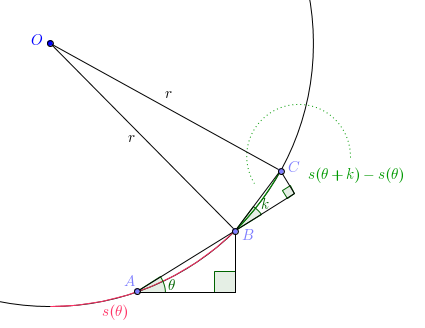
\includegraphics[width=0.6\textwidth]{curvaturecircle}
  \caption{Calculating the curvature of a circle.\label{fig:curvaturecircle}}
\end{figure}

Consider figure \ref{fig:curvaturecircle}. We are approximating a tangent line at $ B $ with the line $ AB $, and then
varying $ \theta $ by a small amount, $ k $. As our secant line $ AB $ approaches a tangent line, the angle at $ B $
between $ AB $ and the radius becomes a right angle. Similarly, the angle at $ C $ with the radius is a right angle for small $ k $. Thus the
angle at $ B $ in the triangle $ OBC $ is approximately $ \pi/2 - k $, and the angle at $ C $ is $ \pi/2 $; thus the angle at $ O $ is $ k $.

We therefore have that $ kr \approx s(\theta + k) - s(\theta) $, and so $ \od{s}{\theta} = r $; therefore $ \kappa = 1/r $.

If $ f $ is some arbitrary function, and we consider the graph $ y = f(x) $, we can calculate $ \od{\theta}{s} $ at each point (we will
do this calculation in a second). At each point, we can associate a circle with the same curvature; this circle is called the \emph{osculating
circle}, the radius $ r $ of the circle is the \emph{radius of curvature} of our graph at that point, and have will say that the \emph{curvature}
of the graph at the point $ x $ is $ \kappa = \od{\theta}{s} = 1/r $.

\begin{figure}
  \centering
  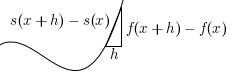
\includegraphics[width=0.3\textwidth]{curvaturefunc}
  \caption{Calculating the curvature of a function.\label{fig:curvaturefunc}}
\end{figure}

So now we will play the same game as above, but now with an arbitrary curve. Consider the function
in figure \ref{fig:curvaturefunc}; we will again denote the angle at $ x $ with the horizontal by $ \theta $.
As we increase $ x $ by $ h $, we increase $ s $ by $ s(x + h) - s(x) $. By definition of the
derivative, $ \od{s}{x} h \approx s(x + h) - s(x) = \sqrt{h^2 + (f(x+h) -f(x))^2} $; dividing through,
\begin{displaymath}
  \od{s}{x} \approx \sqrt{1 + \left(\frac{f(x + h) - f(x)}{h}\right)^2};
\end{displaymath}
and taking the limit $ h \to 0 $, we obtain
\begin{equation}
  \od{s}{x} = \sqrt{1 + \left(\od{y}{x}\right)^2} = \sqrt{1 + \tan^2 \theta} = \sec \theta.\label{eqn:sbyx}
\end{equation}

Furthermore, since $ \od{y}{x} = \tan \theta $ we have
\begin{displaymath}
  \od[2]{y}{x} = \od{}{x} \od{y}{x} = \od{}{x} \tan \theta = \od{\theta}{x} \sec^2 \theta
\end{displaymath}
and hence
\begin{equation}
  \od{x}{\theta} = \frac{\sec^2 \theta}{\left(\od[2]{y}{x}\right)}.\label{eqn:xbyth}
\end{equation}

Finally, by definition we have that the radius of curvature is (combining equations \ref{eqn:sbyx} and \ref{eqn:xbyth})
\begin{displaymath}
  r = \od{s}{\theta} = \od{s}{x} \od{x}{\theta} = \frac{\sec^3 \theta}{\left(\od[2]{y}{x}\right)};
\end{displaymath}
and the curvature is therefore (again by definition)
\begin{displaymath}
  \kappa(x) = \frac{1}{r} = \frac{\od[2]{y}{x}}{\sec^3\theta} = \frac{\od[2]{y}{x}}{\left(\sqrt{1 + \tan^2 \theta}\right)^3}
            = \frac{\od[2]{y}{x}}{\left(1 + \left(\od{y}{x}\right)^2\right)^{3/2}}.
\end{displaymath}


\subsection{Exercises and Problems}
\begin{enumerate}
  \item The following function is known as the \textit{logistic curve} and is used for population modelling. Find the intervals of
        concavity, and label any inflection points.
        \begin{center}
          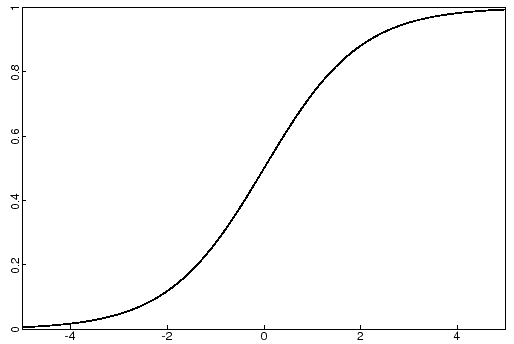
\includegraphics[width=0.4\textwidth]{logistic}
        \end{center}
  \item Find the second derivative of the following functions.
    \begin{enumerate}
      \item $ y = x^2 + x $
      \item $ f(x) = \sin x $
      \item $ g(x) = \cot(3x^2 + 5) $
      \item $ y = \frac{\sin mx}{x} $
      \item $ y = 4 \sin^2 x $
      \item $ y = \tan^2 (\sin \theta) $
      \item $ y = \tan \sqrt{1 - x} $
    \end{enumerate}
  \item Find the concavity of the function $ y = \frac{x^2 - 1}{x^2 + 1} $ at $ (0, -1) $.
  \item Find the intervals on which the following functions are increasing or decreasing, and
        find their intervals of concavity.
    \begin{enumerate}
      \item $ y = x^2 + 1 $
      \item $ y = 2x^3+ 3x^2 - 36x $
      \item $ G(x) = x - 4\sqrt{x} $
    \end{enumerate}
  \item The graph of $ y = f(x) $ (where $ f $ is a continuous function) is concave up for all $ x < 0 $, concave down for $ x > 0 $, and decreasing everywhere.
    \begin{enumerate}
      \item Sketch the graph of $ y = f(x) $.
      \item What can you say about $ f'(x) $ and $ f''(x) $ for $ x < 0 $ and $ x > 0 $?
      \item What about $ x = 0 $?
    \end{enumerate}
  \item Find a value of $ k $ such that the function $ F $ is continuous at $ x = -3 $, where
        \begin{displaymath}
          F(x) =
          \begin{cases}
            \frac{x^2 - 9}{x+3} & \text{if } x \neq -3,\\
            k                   & \text{if } x = -3.
          \end{cases}
        \end{displaymath}
  \item Show whether or not the function $ g $ is continuous at the three points $(2, g(2)) $, $ (3,g(3)) $, and  $(4,g(4)) $, where
        \begin{displaymath}
          g(x) =
          \begin{cases}
            2x-x^2              & \text{if } 0 \leq 2,\\
            2-x                 & \text{if } 2 < x \leq 3,\\
            x-4                 & \text{if } 3 < x \leq 4,\\
            \pi                 & \text{if } x \geq 4.
          \end{cases}
        \end{displaymath}
  \item Find all values of $ \alpha $ such that $ \Phi $ is continuous everywhere, where
        \begin{displaymath}
          \Phi(x) =
          \begin{cases}
            x+1                 & \text{if } x \leq \alpha, \\
            x^2                 & \text{if } x > \alpha.
          \end{cases}
        \end{displaymath}
  \item Sketch a function satisfying the given criteria.
    \begin{enumerate}
      \item
        \begin{itemize}
          \item Vertical asymptote at $ x = 0 $,
          \item $ f'(x) > 0 $ if $ x < -2 $,
          \item $ f'(x) < 0 $ if $ x > -2 $ ($ x \neq 0 $),
          \item $ f''(x) < 0 $ if $ x < 0 $, $ f''(x) > 0 $ if $ x > 0 $.
        \end{itemize}
      \item
        \begin{itemize}
          \item $ f'(0) = f'(2) = f'(4) = 0 $,
          \item $ f'(x) > 0 $ if $ x < 0 $ or $ 2 < x < 4 $,
          \item $ f'(x) < 0 $ if $ 0 < x < 2 $ or $ x > 4 $,
          \item $ f''(x) > 0 $ if $ 1 < x < 3 $,
          \item $ f''(x) < 0 $ if $ x < 1 $ or $ x > 3 $.
        \end{itemize}
    \end{enumerate}
  \item A curve is defined by the function $ f(x) = e^{-(x-k)^2} $. Find, in terms of $ k $, the $ x$-ordinates for which $ f''(x) = 0 $.
  \item It turns out that if a function $ f $ is differentiable at $ a $ then $ f $ is always continuous at $ a $, but the converse
        is not true: there exist continuous functions that are not differentiable. (In fact, there exist functions that are continuous
        everywhere but differentiable nowhere.) \label{exercise:contnotdif}
    \begin{enumerate}
      \item We will prove that differentiability of $ f $ at $ a $ implies continuity of $ f $ at $ a $; expand the following
            and use the limit laws to show that $ \lim_{x \to a} f(x) - f(a) = 0 $, carefully indicating where you use the existence
            of the derivative.
            \begin{displaymath}
              \left[\lim_{a \to x} f(x) - f(a)\right]\left[\lim_{a \to x} \frac{x - a}{x - a}\right]
            \end{displaymath}
      \item Give an example of a function which is continuous but not differentiable at some point.
    \end{enumerate}
  \item We will do some studies of convexity that may be familiar to students who have looked at the exercises on convexity
        in the algebra notes. We assume that all functions are continuous and differentiable everywhere for simplicity.
    \begin{enumerate}
      \item Show that if $ f $ is a convex function, and if $ P = (p,f(p)) $ and $ Q = (q,f(q)) $ are any two distinct points
            on the graph of $ f $, then for every point $ X = (x_1, x_2) $ on the line segment $ \overline{PQ} $, $ x_2 \geq f(x_1) $
            and equality is only obtained at the endpoints.
      \item Show that if $ f $ is a convex function, and if $ P = (p,f(P)) $ is a point on the graph of $ f $, then for every
            point $ (x_1,x_2) $ on the tangent line to $ f $ at $ P $, $ x_2 \leq f(x_1) $ and equality is only obtained at $ P $.
      \item Prove similar statements to (a) and (b) in the case that $ f $ is a concave function. [Hint: there is not much work
            involved, as long as one ponders the function $ -f $.]
    \end{enumerate}
  \item Scholarship 2010: Recall that the points of inflection of a curve are places where the second derivative
        changes sign. These are typically, \textbf{but not always}, points at which the second derivative is zero.

        Consider the curve $ y = \sqrt[3]{x} e^{-x^2} $.

        Write the second derivative in the form $ \od[2]{y}{x} = (ax^4 + bx^2 + x)e^{-x^2} x^{-5/3} $, and hence
        find the $ x$-ordinates of the points of inflection of the curve.
  \item Scholarship 2004: (You may wish to remind yourself how to perform long division of polynomials.) Consider the function
        \begin{displaymath}
          y = \frac{x^2}{1 + x^2},
        \end{displaymath}
        where $ -1 \leq x \leq 1 $. The gradient at the point $ x = 1 $ is $ \frac{1}{2} $.

        Hence show that there is a point with $ \frac{1}{4} \leq x \leq \frac{1}{2} $ where the gradient is also $ \frac{1}{2} $.
  \item Scholarship 2013: A function $ f $ is \textbf{even} if $ f(-x) = f(x) $ for all $ x $ in its domain, and \textbf{odd} if $ f(-x) = f(-x) $
        for all $ x $ in its domain.
    \begin{enumerate}
      \item Describe which polynomials are even, which are odd, and which are neither.
      \item Suppose that $ g $ is any even differentiable function defined for all real numbers (not necessarily a polynomial). Use the
            limit definition of the derivative to prove that $ g' $ is odd.
    \end{enumerate}
  \item Recall that we can define the derivative of $ f $ by $ \mathsf{D}f(x) = \lim_{y \to x} \frac{f(y) - f(x)}{y - x} $.
        We will generalise this, by writing $ \mathsf{SD}f(x) = \lim_{h \to 0} \frac{f(x + h) - f(x - h)}{2h} $.
        This is called the \emph{symmetric derivative} of $ f $.
    \begin{enumerate}
      \item In fact, we defined the derivative of $ f $ at $ x $ to be the unique $ f' $ such that $ f(x + h) \approx f(x) + hf'(x) $
            for small $ h $.\footnote{Then we defined the notation $ \varphi(x,h) \approx \psi(x,h) $ to mean that $ \varphi(x) = \psi(x) + \vartheta(h) $
            for some function $ \vartheta $ satisfying $ \vartheta(h)/h \to 0 $ as $ h \to 0 $.}

            Show that, for small $ h $, if $ f'(x) $ exists then $ f(x + h) - f(x - h) \approx 2hf'(h) $. Hence
            conclude that $ \mathsf{SD}f(x) = \mathsf{D}f(x) $ whenever the latter exists.
      \item The converse is not true: show that if we define $ f(x) = \abs{x} $, then $ \mathsf{SD} f(0) $ exists
            but $ \mathsf{D} f(0) $ does not.
      \item Define the \emph{second} symmetric derivative of $ f $ by
            \begin{displaymath}
              \mathsf{SD}^2 f(x) = \lim_{h \to 0} \frac{\frac{f(x + h) - f(x)}{h} - \frac{f(x) - f(x - h)}{h}}{h} = \lim_{h \to 0} \frac{f(x + h) - 2f(x) + f(x - h)}{h^2}.
            \end{displaymath}
            Show that whenever $ f''(x) = \mathsf{D}^2 f(x) $ exists then $ \mathsf{SD}^2 f(x) $ exists and has the same value; show that the converse
            does not hold (i.e. the existence of the second symmetric derivative does not imply the existence of the usual second derivative)
            by considering a suitable function, such as
            \begin{displaymath}
              \mathrm{sgn}(x) = \begin{cases} -1 & x < 0 \\ 0 & x = 0 \\ 1 & x > 0. \end{cases}
            \end{displaymath}
    \end{enumerate}
  \item One may recall from one of the L1 externals that we can recover a quadratic equation given a table of its values. Suppose
        we know that the following table gives points on the graph of $ f(x) = ax^2 + bx + c $.

        \begin{tabular}{c|c}
          $ x $ & $ f(x) $ \\
          $ 0 $ & $ -5 $ \\
          $ 1 $ & $ 2 $ \\
          $ 2 $ & $ 15 $
        \end{tabular}

        Define the \emph{discrete first and second derivatives} of $ f $ by $ \Delta f(x) = f(x + 1) - f(x) $ and $ \Delta^2 f(x) = \Delta f(x + 1) - \Delta f(x)  $.
        According to the god-given material in L1, we know that if $ f $ is a quadratic, then $ a = \frac{1}{2} \Delta^2 f(x) $ (for any choice of $ x $); in this
        example, we can fill in the table as follows:-

        \begin{tabular}{c|c|c|c}
          $ x $ & $ f(x) $ & $ \Delta f(x) $ & $ \Delta^2 f(x) $\\
          $ 1 $ & $ -5 $ & $ 7 $ & $ 6 $\\
          $ 2 $ & $ 2 $ & $ 13 $ & \\
          $ 3 $ & $ 15 $ &&
        \end{tabular}

        Hence $ a = 3 $. We can then write (since we know $ f $ is a quadratic) $ bx + c = f(x) - 3x^2 $, which tells us that $ b\cdot 1 + c = -8 $
        and $ b \cdot 2 + c = -10 $; hence $ b = (-10 - {}^{-}8)/1 = -2 $ and $ c = -6 $. \label{exercise:funtimeswithcalculus}

        \begin{enumerate}
          \item Justify the above steps. (Possible approach: $ hf''(x) \approx f'(x + h) - f'(x) $; set $ h = 1 $, and work out what fudge
                factor $ \vartheta(h) $ we have.)
          \item Develop a theory of discrete first and second derivatives. (Possible routes of study could include: finding a geometric
                meaning of the discrete derivatives; defining discrete $ n$th derivatives; studying the relationship between the discrete
                derivatives and the usual derivatives. You may also want to generalise my definition: instead of $ f(x + 1) - f(x) $,
                perhaps one might like to look at $ [f(x + k) - f(x)]/k $ (sans limit).)
        \end{enumerate}
  \item These problems relate to the optional section on curvature and arc length.
    \begin{enumerate}
      \item If $ y = f(x) $, formula \ref{eqn:sbyx} gives us the derivative of arc length with respect to distance
            along the $ x$-axis. What is the arc length along the graph of the function $ f(x) = \frac{1}{3}x^3 - x $
            between the vertical lines $ x = 0 $ and $ x = 5 $?
      \item Repeat (a) for the function $ g(x) = \ln \abs{\sec x} $.
      \item What is the curvature of a straight line?
      \item Calculate the curvature $ \kappa(x) $ of the function $ f(x) = x^2 $ at the points $ x = 0 $, $ x = 2 $, and $ x = 4 $.
            Draw the osculating circles at each of these points. What happens to $ \kappa(x) $ as $ x \to \infty $?
    \end{enumerate}
\end{enumerate}

\subsection{References}
A good introduction to the geometry of curves, and differential geometry in general, is \emph{Differential Geometry
of Curves and Surfaces} by Manfredo P. do Carmo.

For a discussion of the history of continuity, see J F Harper (2016): Defining continuity of
real functions of real variables, BSHM Bulletin: Journal of the British Society for the History
of Mathematics, DOI:10.1080/17498430.2015.1116053 (\url{http://homepages.ecs.vuw.ac.nz/~harper/harper16.pdf}).

Discrete derivatives (see exercise \ref{exercise:funtimeswithcalculus}) are useful when taking
derivatives numerically (say we have a table of numbers defining a function $ f $, but we don't
have a nice formula for it). The kinds of things one may want to search for in a library catalogue
are ``difference calculus'' or ``discrete calculus''.

\subsection{Homework problems}
\begin{enumerate}
  \item Explain, with sketches, the geometric meaning of the second derivative.
  \item Find the second derivative of the following functions.
    \begin{enumerate}
      \item $ f(x) = x^5 - 5x + 3 $
      \item $ f(x) = \frac{x^2}{x - 1} $
      \item $ f(x) = \sqrt{x} - \sqrt[4]{x} $
    \end{enumerate}
  \item Sketch a function satisfying the given criteria.
    \begin{enumerate}
      \item (hint: your result should be an odd function)
        \begin{itemize}
           \item $ f'(1) = f'(-1) = 0 $,
           \item $ f'(x) < 0 $ if $ \abs{x} < 1 $,
           \item $ f'(x) > 0 $ if $ 1 < \abs{x} < 2 $,
           \item $ f'(x) = -1 $ if $ \abs{x} > 2 $.
        \end{itemize}
      \item
        \begin{itemize}
          \item $ f'(x) < 0 $,
          \item $ f''(x) < 0 $.
        \end{itemize}
    \end{enumerate}
\end{enumerate}

\section{Optimisation problems}
Suppose we need to choose a rectangle with a fixed perimeter, but a maximal area. By considering the
symmetry of the problem, it is almost clear that if a solution exists then it \emph{should} be a square.

Indeed, suppose that our rectangle has side lengths $ x $ and $ y $, and perimeter $ \mathcal{P} $. Then $ \mathcal{P} = 2(x + y) $,
and so the area of our rectangle (the quantity we wish to maximise) is
\begin{displaymath}
  \mathcal{A} = xy = \frac{x(\mathcal{P} - 2x)}{2} = \frac{1}{2}\mathcal{P}x - x^2.
\end{displaymath}
Noting that the graph of the function $ \mathcal{A}(x) $ is a parabola, opening downwards, it is clear
that our desired maximum is the vertex; completing the square, we find that
\begin{displaymath}
  \mathcal{A} = \frac{1}{16}\mathcal{P}^2 - \left(x - \frac{1}{4}\mathcal{P}\right)^2
\end{displaymath}
and thus the vertex has $ x$--value $ \mathcal{P}/4 $; immediately, $ x = y $ and we see that our guess,
of a square optimal shape, was correct.

We were able to solve this problem because it ended up being equivalent to finding the maximum of a quadratic,
which is easy to solve in this way with only a little effort. However, consider the following problem, which is
essentially the same but now in three dimensions:
\begin{pro}
  Suppose a rectangular prism has two square faces of side length $ x $, and four rectangular faces with side lengths $ x $
  and $ y $; so the volume of the prism is $ x^2 y $. Let the perimeter $ \mathcal{P} = 8x + 4y $ of the prism be fixed.
  Find $ x $ and $ y $ satisfying this constraint such that the volume is maximised.
\end{pro}
Considering $ V = x^2y $, we substitute in our constraints:
\begin{displaymath}
  V = x^2 \left( \frac{\mathcal{P} - 8x}{4} \right) = \frac{\mathcal{P}}{2} x^2 - 2x^3
\end{displaymath}
and now we need to find the maximum value of a cubic --- which is not something we can do easily geometrically.

These types of problems are our motivation for the study in this section.

\begin{defn}
  If $ f $ is a function, then $ f $ is said to have a \emph{local maximum} at $ x_0 $ if there exists some (small)
  number $ \delta $ such that, for all $ x $ between $ x_0 - \delta $ and $ x_0 + \delta $, $ f(x) \leq f(x_0) $.

  Similarly, $ f $ is said to have a \emph{local minimum} at $ x_0 $ if there exists some number $ \delta $ such that,
  for all $ x $ between $ x_0 - \delta $ and $ x_0 + \delta $, $ f(x) \geq f(x_0) $.

  Local maxima and local minima are, collectively, called \emph{local extrema}. If we can take $ \delta $ as large
  as we like in either definition (e.g. if $ f(x) \geq f(x_0) $ for all possible $ x $ anywhere in the real numbers),
  we replace `local' with \emph{global}.

  For an illustration, see figure \ref{fig:localmin}.
\end{defn}

Many optimisation problems in applied mathematics can be reduced to finding relative extrema.

\begin{figure}
  \centering
  \begin{tikzpicture}
    \begin{axis}[
      axis lines = none,
      xlabel = $ x $,
      ylabel = {$ y = f(x) $}
    ]
      \addplot[domain = -3:3, color = black, samples = 100] {(1/6)*x^3 - (1/2)*x};
      \node[circle,fill,inner sep=2pt] at (axis cs:1,-1/3) {};
      \node[label={above:{$\left(x_0,f(x_0)\right)$}},circle,fill,inner sep=2pt] at (axis cs:1,-1/3) {};
      \draw[color=black!40, style=dotted] (0.15,-2) -- (0.15,2);
      \draw[color=black!40, style=dotted] (1.85,-2) -- (1.85,2);
      \node[label={below:{$x_0 - \delta$}}] at (axis cs:0.15,-2) {};
      \node[label={below:{$x_0 + \delta$}}] at (axis cs:1.85,-2) {};
    \end{axis}
  \end{tikzpicture}
  \caption{A local minimum of $ f $ at $ x_0 $ is a point lower than every other point in some interval around it.\label{fig:localmin}}
\end{figure}

\begin{exs}\leavevmode
  As in our first example above, many functions have local extrema that can be found with a little intelligent thought.
  \begin{enumerate}
    \item The function $ x \mapsto x^2 $ has a local minimum at $ (0, 0) $.
    \item The function $ x \mapsto 2x^3 + 15x^2 + 36x + 2 $ has a local maximum at $ (-3, -25) $ and a local minimum at $ (-2, -26) $.
    \item The function $ x \mapsto \sin x $ has a local maximum at $ (2n\pi + \frac{\pi}{2}, 1) $ for every integer $ n $, and
          a local minimum at $ (2n\pi - \frac{\pi}{2}, 1) $ for every integer $ n $.
  \end{enumerate}
\end{exs}

The main theorem is the following, which is a simple extension of the ideas from the last section on the geometry of the graphs
of functions. The basic geometric idea is that at a local extrema, the graph is changing from increasing to decreasing (or vice versa)
and thus the derivative is changing from a positive value to a negative value (or vice versa), and so must pass through zero.

\begin{thm}[Fermat]
  Let $ f $ be a function; suppose $ x_0 $ is a point in the interior of the domain of $ f $ (i.e. $ f(x) $ is defined for all $ x $ close
  to $ x_0 $ on both sides), that $ f $ is differentiable at $ x_0 $, and that $ f $ has a relative extremum  at $ x_0 $. Then $ f'(x_0) = 0 $.
\end{thm}
\begin{proof}
  Suppose $ x_0 $ is a local maximum of $ f $. Then for all $ x < x_0 $ such that $ x $ is `sufficiently close'\footnote{i.e. $ x $ lies
  within the $ \delta$-interval in the definition of a local maximum} to $ x_0 $, $ f(x) \leq f(x_0) $. Thus
  \begin{displaymath}
    \frac{f(x_0) - f(x)}{x_0 - x} \geq 0,
  \end{displaymath}
  since it is the quotient of two non-negative numbers.

  Similarly, for all $ x > x_0 $ sufficiently close to $ x_0 $, $ f(x) \leq f(x_0) $ and so
  \begin{displaymath}
    \frac{f(x_0) - f(x)}{x_0 - x} \leq 0.
  \end{displaymath}

  Since $ \lim_{x \to x_0} \frac{f(x_0) - f(x)}{x_0 - x} $ exists, the quantity $ \frac{f(x_0) - f(x)}{x_0 - x} $ must
  tend to the same value whether we approach from the left or from the right; and the only possible such value is zero.
\end{proof}

Motivated by this theorem, we define a \emph{critical point} of a function $ f $ to be some value $ x $ in the domain of $ f $ such
that either $ f'(x) = 0 $, or $ f'(x) $ is undefined. In the first case, we also call the value a \emph{stationary point}. All local
extrema occur at critical points, but not all critical points occur at extrema.

\begin{exs}\leavevmode
  \begin{enumerate}
    \item The function $ x \mapsto 2x^3 + 15x^2 + 36x + 2 $ above has critical points $ x = -2 $ and $ x = -3 $. Both of
          these are local extrema.
    \item The function $ x \mapsto x^3 $ above has a critical point at $ x = 0 $, but does not have a local extrema there.
    \item The function $ x \mapsto \frac{1}{x} $ \textbf{does not} have a critical point at $ x = 0 $, \textbf{because it is not defined there}.
  \end{enumerate}
\end{exs}

Utilising this technique, we can write down a recipe like the following to find extrema of a function $ f $ mechanically:
\begin{enumerate}
  \item Compute $ f' $.
  \item Find the points where $ f $ is defined but $ f' $ is not
  \item Find all the points where $ f' $ is zero.
  \item Find all the points $ x $ where $ f $ is defined at $ x $ and all points on one side of $ x $, but not the other.
  \item Then all the local extrema of $ f $ will be included in the lists of points in (2)--(3), and so we check each
        manually.
\end{enumerate}

There are two problems with this recipe. Firstly, the list of possible extrema may include points which are not actually
extrema and so we need a way to decide quickly whether a point is an extrema or a false alarm. This is something we will
address in a moment, so a more pressing concern is the second: finding zeroes of a function, in this case $ f' $, is just
as hard as finding extrema --- so we are only replacing one difficult problem with another.

\subsection{The geometry of critical points}
We can use the first derivative to classify extrema as either maxima or minima.
\begin{enumerate}
  \item Determine all critical points of $ f $.
  \item Determine the sign of $ f'(x) $ to the left and right of each critical point $ x_0 $:
    \begin{itemize}
      \item If $ f'(x) $ changes from positive to negative as we move from left to right across $ x_0 $, then $ f(x) $ has a local maximum at $ x_0 $.
      \item If $ f'(x) $ changes from negative to positive as we move from left to right across $ x_0 $, then $ f(x) $ has a local minimum at $ x_0 $.
      \item If $ f'(x) $ does not change sign across $ x_0 $, then $ f(x) $ does not have a relative extremum at $ x_0 $ (e.g. $ y = x^3 $).
    \end{itemize}
\end{enumerate}

On the other hand, using the second derivative, we can come up with a different test:
\begin{enumerate}
  \item Compute $ f'(x) $ and $ f''(x) $.
  \item Find all the stationary points of $ f $ by finding all the points $ x_0 $ such that $ f'(x_0) = 0 $.
  \item Determine the sign of $ f''(x) $ for each stationary point $ x_0 $:
    \begin{itemize}
      \item If $ f''(x_0) < 0 $ (i.e. $ f $ is concave down), then $ f(x) $ has a relative maximum at $ x_0 $.
      \item If $ f''(x_0) > 0 $ (i.e. $ f $ is concave up), then $ f(x) $ has a relative minimum at $ x_0 $.
      \item If $ f''(x_0) = 0 $ (i.e. $ f $ has an inflection point at $ x_0 $), then $ f(x) $ could have a relative maximum, a relative minimum, or neither.
    \end{itemize}
\end{enumerate}

\begin{ex}
  Find and classify the critical points of $ y = x^3 - 3x^2 + 6 $.

  \textit{Solution.} We have $ \od{y}{x} = 3x^2 - 6x $ and $ \od[2]{y}{x} = 6x - 6 $. Hence
                     the critical points are $ x = 0 $ and $ x = 2 $. At the former point, $ \od[2]{y}{x} < 0 $,
                     and so the point is a maximum; at the latter point, $ \od[2]{y}{x} > 0 $ and so the point is
                     a minimum.
\end{ex}

\begin{ex}
  Find two numbers whose difference is 100 and whose product is a minimum.

  \textit{Solution.} Let the two numbers be $ x $ and $ x + 100 $. We wish to minimise $ y = x(x + 100) $;
  clearly $ y' = 2x + 100 $, and so $ x = -50 $ is a critical point. To the left of $ x = -50 $, the derivative
  is negative; to the right, the derivative is positive. Hence $ x = -50 $ is indeed a minimum. The two required
  numbers are therefore -50 and 50.
\end{ex}

\begin{ex}
  Find and classify the critical points of $ y = (x - 1)^2 + \ln x $.

  \textit{Solution.} The derivative is $ y' = 2x - 2 + \frac{1}{x} $. We therefore have one critical
  point at $ x = 0 $ (where $ y' $ is undefined); this is an asymptote.
  Setting $ y' = 0 $, we have $ 0 = 2x - 2 + \frac{1}{x} = 2x^2 - 2x + 1 $ which has no real roots. Hence $ x = 0 $ is
  the only critical point, and the curve has no local extrema.
\end{ex}

\begin{ex}
  A rectangular plot of land is to be fenced using two varieties of fence. Two opposite sides will
  use fences selling for \$3 per metre, while the other two sides will use cheaper fence selling for \$2 per metre.
  Given that the total budget is \$1200, what is the greatest area of land which can be fenced?

  \textit{Solution.} Let $ x $ be the length of one of the expensive sides; then the length of one of the cheaper
                    sides is $ \frac{1}{2}(1200 - 3x) $, and the total area is $ A = \frac{1}{2} x (1200 - 3x) = \frac{1}{2}(1200x - 3x^2) $.
                    Hence $ \od{A}{x} = 600 - 3x $. We wish to find the maximum area, so set $ \od{A}{x} = 0 $; hence $ 3x = 600 $ and $ x = 200 $.
                    Note that the second derivative is always negative, so this stationary point must be a maximum as required. The length
                    of the other side will be $ \frac{1}{2}(1200 - 600) = 300 $, and so the maximum area is $ 300 \times 200 = 60000 $ square metres.
\end{ex}

\subsection{Exercises and Problems}
\begin{enumerate}
  \item Describe the advantages and disadvantages of the first and second derivative tests for local extrema.
  \item Describe the local extrema, concavity, and points of inflection of the function $ f(x) = x^4 - 4x^3 $.
  \item Consider the following graph:
        \begin{center}
          \begin{tikzpicture}[scale=.8]
            \begin{axis}[
              axis lines = center,
              xlabel = $ x $,
              ylabel = {$ y = f(x) $}
            ]
              \addplot[domain = -0.5:4, color = black, samples = 100] {x^3 - 4*x^2 + 3*x};
              \node[label={above:{$C$}},circle,fill,inner sep=2pt] at (axis cs:2.22,-2.11) {};
              \node[label={below:{$B$}},circle,fill,inner sep=2pt] at (axis cs:1.33,-0.74) {};
              \node[label={above:{$A$}},circle,fill,inner sep=2pt] at (axis cs:0.45,0.63) {};
            \end{axis}
          \end{tikzpicture}
        \end{center}
        Find the signs of $ \od{y}{x} $ and $ \od[2]{y}{x} $ at the three points $ A $, $ B $, and $ C $.
  \item Find all the local extrema of the following curves in the given intervals, and classify them as maxima, minima, or neither.
    \begin{enumerate}
      \item $ f(x) = \sin x - \cos x $ on the interval $ 0 < x < \pi $
      \item $ g(x) = x^3 - x^2 + x - 1 $ on the interval $ -\infty < x < \infty $
    \end{enumerate}
  \item The sum of two positive numbers $ x $ and $ y $ is 16. Find the smallest possible value for $ S = x^2 + y^2 $.
  \item A box with an open top is to be constructed from a square piece of cardboard with a side length of \SI{3}{\metre}
        by cutting out a square from each of the four corners and bending up the sides. Find the dimensions of the resultant
        box of maximum volume.
  \item Find the dimensions of a rectangle with area \SI{1000}{\metre\squared} such that the perimeter is minimised.
  \item A window consisting of a rectangle topped with a semicircle is to have a fixed perimeter $ p $. Find the radius
        of the semicircle in terms of $ p $ if the total area is to be maximised.
  \item A thin wire of length $ L $ is cut in two and the resulting lengths are bent to make a square and an equilateral triangle. Where
        should the wire be cut to make the total area of the shapes (a) a maximum and (b) a minimum?
  \item Find the point on the line $ y = 2x + 3 $ closest to the origin.
  \item Find the point on the curve $ y = \sqrt{x} $ closest to $ (3, 0) $.
  \item By finding the $ x$-- and $ y$-- intercepts, the asymptotes, the critical points, the
        intervals of increase and decrease, the intervals of concavity, and any other important
        points, sketch the following functions (199):
    \begin{enumerate}
      \item $ f(x) = \frac{x^2}{4 - x^2} $
      \item $ f(x) = \frac{4x}{x^2 + 1} $ [\textit{Hint: consider what happens to $ f(x) $ as $ x \to \pm\infty $.}]
      \item $ f(x) = \frac{x^2 - 4x + 5}{x - 2} = x - 2 + \frac{1}{x - 2} $ [\textit{Hint: consider what happens to $ f(x) - (x - 2) $ as $ x \to \pm\infty $.}]
    \end{enumerate}
  \item A cone with height $ h $ is inscribed in a larger cone of height $ H $ such that the vertex of the small cone
        is at the centre of the base of the larger cone. Show that the maximum volume of the smaller cone occurs when $ h = \frac{1}{3} H $.
  \item Show that the polynomial $ p(x) = 10x^3 + x^2 + x - 34 $ has exactly one real zero.
  \item A rain gutter is to be constructed from a metal sheet of width \SI{30}{\centi\metre} by bending up
        one third of the sheet on each side by an angle $ \theta $. What angle should be chosen in order to
        obtain the maximum possible volume?
  \item A steel pipe is carried around a right-angled corner from a hallway \SI{3}{\metre} wide into a hallway \SI{2}{\metre}
        wide. What is the length of the longest pipe that can be carried horizontally around the corner? [\textit{Hint: this is actually
        a minimisation problem, despite the wording.}]
  \item A large orange rectangle is to be drawn with one corner sitting on the origin and the opposite corner lying on
        the curve $ y = 0.2(x - 10)^2 $. What is the maximum possible area of the rectangle?
        \begin{center}
          \begin{tikzpicture}[scale=.8]
            \begin{axis}[
              axis lines = center,
              xlabel = $ x $,
              ylabel = {$ y = f(x) $}
            ]
              \draw[fill = orange] (0,0) rectangle (3,9.8);
              \addplot[domain = -1:15, color = black, samples = 100] {0.2*(x - 10)^2};
            \end{axis}
          \end{tikzpicture}
        \end{center}
  \item Show that $ \frac{x^2 + 1}{x} \geq 2 $; hence (or otherwise) show that $ \frac{(x^2 + 1)(y^2 + 1)(z^2 + 1)}{xyz} \geq 8 $.
  \item Scholarship 2013: Prince Ruperts drops are made by dropping molten glass into cold water. A mathematical model for a drop
        as a volume of revolution uses $ y = \sqrt{\phi (e^{-x} - e^{-2x})} $ for $ x \geq 0 $, where $ \phi $ is the golden
        ratio $ \phi = \frac{1 + \sqrt{5}}{2} $.
    \begin{enumerate}
      \item Where is the modelled drop widest, and how wide is it there?
      \item The drop changes shape at a point $ B $, where the concavity of the function is zero. Use
            \begin{displaymath}
              \od[2]{y}{x} = \sqrt{\phi} \frac{e^{2x} - 6e^x + 4}{y^2 e^{4x}}
            \end{displaymath}
            to find the exact $ x$-ordinate of $ B $.
    \end{enumerate}
  \item Scholarship 2014: A family of functions is built from two functions $ f $ and $ g $, with a new function $ h_p $ defined
        for each value of $ p $, $ 0 \leq p \leq 1 $:
        \begin{gather*}
          f(x) = 2 + \sin x\\
          g(x) = 26 + \sin x\\
          h_p(x) = [f(x)]^{1 - p} [g(x)]^p.
        \end{gather*}
        Define a fourth function $ S $, where $ S(p) $ is the difference between the maximum and the minimum values of $ h_p $. Find
        the exact value of $ p $ that maximises $ S $.

        Note that if $ a $ is constant, $ \od{}{x} a^x = (\ln a) a^x $.
  \item Note that the second-derivative test may be inconclusive: if $ f'(x_0) = 0 $, and $ f''(x_0) = 0 $, then we may have
        an inflection point (like in the case of $ x \mapsto x^3 $), or a local extrema (like $ x \mapsto x^4 $). Looking at
        the second example here, one might conjecture that if we have a local extrema then $ f^{(n)}(x_0) > 0 $ for some large
        enough $ n $ (in the case of $ x^4 $, the fourth derivative is positive).

        Define $ f $ by
        \begin{displaymath}
          f(x) = \begin{cases} e^{-1/x^2} & x \neq 0 \\ 0 &x = 0 \end{cases}.
        \end{displaymath}
    \begin{enumerate}
      \item Show that $ f $ is differentiable at zero.
      \item Show that, for all $ n > 0 $, $ f^{(n)}(0) = 0 $. (Implicit here is the existence of the $ n$th derivative.)
      \item Show that $ f $ has a global minimum at zero.
      \item Justify that there can thus never be a rule, based simply on checking $ n$th derivatives, for proving
            that any function has a local minimum or maximum at a point. Hence our conjecture is false.
      \end{enumerate}
  \item Find $ x $, $ y $, and $ z $ positive real numbers such that the volume $ V = xyz $
        of the rectangular prism with these sidelengths is maximised, given that the perimeter
        of the prism is $ 4x + 4y + 4z = 12 $ and the surface area is $ 2xy + 2yz + 2zx = 6 $.
\end{enumerate}

\subsection{References}
For a significant number of optimisation exercises of the mechanical sort, see Stewart sections 4.1 and 4.7.

For more interesting problems, see Spivak chapter 11.

One avenue for further reading is the subject of the calculus of variations. See, for example, L\&S section 3.15,
as well as (for example) \emph{An introduction to the Calculus of Variations}, by Hans Sagan (Dover, 1992).

\subsection{Homework}
\paragraph{Reading}


\paragraph{Problems}
\begin{enumerate}
  \item What is the minimum vertical distance between the parabolae $ y = x^2 + 1 $ and $ y = x - x^2 $?
  \item Show that $ 3x + 2\cos x + 5 = 0 $ has exactly one real root by showing that it
        is increasing everywhere and crosses the $ x$-axis somewhere between two values of $ x $.
  \item Find the area of the largest rectangle that can be inscribed in the ellipse $ \frac{x^2}{a^2} + \frac{y^2}{b^2} = 1 $.
  \item Let $ ABCD $ be a square piece of paper with sides of length \SI{1}{\metre}. A
        quarter-circle is drawn from $ B $ to $ D $ with centre $ A $. The piece of paper is folded along $ EF $, with $ E $ on $ AB $
        and $ F $ on $ AD $, so that $ A $ falls on the quarter-circle. Determine the maximum and minimum areas that the triangle $ AEF $
        can have. [\textit{Hint: you may want to introduce a coordinate system.}]
\end{enumerate}

\section{Approximations}
Our original definition of the derivative was motivated in part by finding the `best'
linear approximation to a curve at a given point. Indeed, if $ f $ is a function then,
for all $ h $ such that $ f(x_0 + h) $ is defined, we have
\begin{displaymath}
  f(x_0 + h) - f(x_0) = h f'(x_0) + \vartheta(h)
\end{displaymath}
where $ \lim_{h \to 0} \vartheta(h)/h = 0 $; in particular, for any $ x $ where $ f $
is defined (moreover, we need $ f $ to be defined everywhere \emph{between} $ x $ and $ x_0 $)
we have
\begin{displaymath}
  f(x) - f(x_0) = (x - x_0) f'(x_0) + \vartheta(x - x_0)
\end{displaymath}
where we have simply replaced $ h $ with $ x - x_0 $. We already defined the tangent
line to $ f $ at $ x_0 $ to be the line given by $ y - f(x_0) = (x - x_0) f'(x_0) $;
so the above equation tells us that if $ (x,y) $ is on the tangent line then
\begin{align*}
  f(x) - y = [(x - x_0) f'(x_0) + \vartheta(x - x_0) + f(x_0)] - [(x - x_0)f'(x_0) + f(x_0)] = \vartheta(x - x_0)
\end{align*}
and so we have that
\begin{displaymath}
  \frac{f(x) - y}{x - x_0} = \frac{\vartheta(x - x_0)}{x - x_0} \xrightarrow{x - x_0 \to 0} 0:
\end{displaymath}
in other words, as we move our point $ x $ of interest closer and closer to $ x_0 $, the `error' in
the tangent line approximation vanishes at a faster rate than our movement. Figure \ref{fig:approx1}
illustrates these relationships; notice that at points $ x $ close to the point of tangency (in this case $ x_0 = 2 $),
$ \tilde f(x) - f(x) $ is approaching zero faster than the distance $ \abs{x - x_0} $.

\begin{figure}
  \centering
  \begin{tikzpicture}[scale = 1.5]
    \begin{axis}[
      axis lines = center,
      xlabel = $ x $,
      ylabel = {$ y $},
    ] %(x -2)(x - 3) + (x + 1)(x - 3) + (x + 1)(x - 2) = x^2 - 5x + 6 + x^2 - 2x - 3 + x^2 - x - 2 = 3*16 - 2*16 + 1
      \addplot[domain = -0.5:3.5, color = black, samples = 100] {(x + 1)*(x - 2)*(x - 3) + 2};
      \addplot[domain = -0.5:3.5, color = red, samples = 5] {-3*(x - 2) + 2};
      \addplot[domain = -0.5:3.5, color = blue, samples = 100] {((x + 1)*(x - 2)*(x - 3) + 2) - (-3*(x - 2) + 2) };
      \addplot[domain = -0.5:2, color = green, samples = 5] { 2-x };
      \addplot[domain = 2:3.5, color = green, samples = 5] { x-2 };
    \end{axis}
  \end{tikzpicture}
  \caption{The graph of a function $ f(x) $ (black), its tangent line $ \tilde f(x) $ at $ 2 $ (red), $ f(x) - \tilde f(x) $ (blue), and $ y = \abs{x - 2} $ (green).\label{fig:approx1}}
\end{figure}

Given that the tangent line is, in this sense, a good linear approximation, it is natural to ask the following question:
\begin{center}\itshape
  If $ f $ is differentiable at $ x_0 $, what is the best polynomial approximation to $ f $ around the point $ x_0 $?
\end{center}

As a reminder, a polynomial is a function $ p $ of the form $ p(x) = p_n x^n + p_{n - 1} x^{n - 1} + \cdots + p_1 x + p_0 $
where $ p_n \neq 0 $. The various $ p_k $ are called the \emph{coefficients}, and $ n $ is the \emph{degree} of $ p $.

This question is an important one, because if we can answer it then we can always replace differentiable functions (which
are difficult to calculate --- what is $ \sin(32.341) $?) with polynomials (which only require a finite number of multiplications
and additions to calculate) with only a small loss of information.

One important use for this is in physics; we will see later on (when we look at differential equations) that in order to
model something like a swinging pendulum, we need to justify why $ \sin x \approx x $ for small $ x $. In engineering
applications too, it is often useful to replace complicated sums and products of things like trig functions with quadratics
and cubics that have the same `shape' around a given point of interest but are much easier to calculate with.

Our plan of attack will be, given a function $ f $ that is differentiable (at least) $ n $ times at some point $ x_0 $,
to find a polynomial
\begin{displaymath}
  p(x) = p_n (x - x_0)^n + p_{n - 1} (x - x_0)^{n -1} + \cdots + p_1 (x - x_0) + p_0
\end{displaymath}
satisfying the following conditions:
\begin{align*}
  p(x_0) &= f(x_0)\\
  p'(x_0) &= f'(x_0)\\
  &\vdots\\
  p^{(n)}(x_0) &= f^{(n)}(x_0).
\end{align*}
(For convenience, the zeroth derivative of $ f $ is $ f $ itself.)

Our argument above shows that the linear polynomial approximation at $ x_0 $ is $ p(x) = f'(x_0)(x - x_0) + f(x_0) $. We will need the following lemma:

\begin{lemma}
  Let $ p(x) = p_n (x - x_0)^n + p_{n - 1} (x - x_0)^{n -1} + \cdots + p_1 (x - x_0) + p_0 $ be a polynomial. Then $ p_k = \frac{p^{(k)}(x_0)}{k!} $
  for all $ 0 \leq k \leq n $.
\end{lemma}
\begin{proof}
  We have the following:
  \begin{align*}
    p(x) = p_n (x - x_0)^n + \cdots + p_3 (x - x_0)^3 + p_2 (x - x_0)^2 + p_1 (x - x_0) + p_0 &\implies p(x_0) = p_0\\
    p'(x) = n p_n (x - x_0)^{n-1} + \cdots + 3p_3 (x - x_0)^2 + 2p_2 (x - x_0) + p_1 &\implies p'(x_0) = p_1\\
    p''(x) = n(n - 1) p_n (x - x_0)^{n - 2} + \cdots + (3 \cdot 2)p_2 (x - x_0) + 2p_2 & \implies p''(x_0) = 2p_2\\
    p^{(3)}(x) = n(n - 1)(n - 2) p_n (x - x_0)^{n - 3} + \cdots + (3 \cdot 2)p_2 & \implies p^{(3)}(x_0) = (2 \cdot 3)p_3\\
  \end{align*}
  and in general, completing the pattern,
  \begin{displaymath}
    p^{(k)}(x_0) = (k!)p_k.
  \end{displaymath}
\end{proof}

Thus, if we want to match $ f $ with a polynomial of degree $ n $ such that $ f^{(k)}(x_0) = p^{(k)}(x_0) $
for every $ 0 \leq k \leq n $ we simply choose $ p(x) = p_n (x - x_0)^n + p_{n - 1} (x - x_0)^{n -1} + \cdots + p_1 (x - x_0) + p_0 $
such that
\begin{displaymath}
  p_k = \frac{f^{(k)}(x_0)}{k!}.
\end{displaymath}
This polynomial is called the $ n$th \emph{Taylor polynomial} of $ f $ at $ x_0 $; we might even write $ \mathsf{T}_{n, x_0} f $
for this polynomial.

\begin{ex}0, 1, 0, -1, 0, 1,
  Consider $ f(x) = \sin x $. Then $ f^{(0)}(0) = 0 $, $ f^{(1)}(0) = 1 $, $ f^{(2)}(0) = 0 $, $ f^{(3)}(0) = -1 $, and in general
  \begin{displaymath}
    f^{(n)}(0) = \begin{cases*}
                   0 & $ n $ even\\
                   (-1)^{k} & $ n = 2k + 1 $ odd
                 \end{cases*}
  \end{displaymath}

  In particular, $ \mathsf{T}_{2k + 1, 0} f = x - \frac{1}{3!} x^3 + \frac{1}{5!} x^5 - \frac{1}{7!} x^7 + \cdots + \frac{(-1)^k}{(2k + 1)!}x^{2k + 1} $;
  the Taylor polynomials for $ k = 0 $ (red), $ k = 1 $ (green), and $ k = 2 $ (blue) are graphed in figure \ref{fig:approx2}.
  \begin{figure}
    \centering
    \begin{tikzpicture}
      \begin{axis}[
        axis lines = center,
        xlabel = $ x $,
        ylabel = {$ y $},
        ymax = 4,
        ymin = -4
      ]
        \addplot[domain = -pi:pi, color = black, samples = 50] { sin(deg(x)) };
        \addplot[domain = -pi:pi, color = red, samples = 50] { x };
        \addplot[domain = -pi:pi, color = green, samples = 50] { x - (1/6)*x^3 };
        \addplot[domain = -pi:pi, color = blue, samples = 50] { x - (1/120)*x^5 };
      \end{axis}
    \end{tikzpicture}
    \caption{The first few Taylor polynomials of sine.\label{fig:approx2}}
  \end{figure}
\end{ex}

We can even do the same error estimation that we performed above, although it is a little tedious; we
find that
\begin{equation}\label{eqn:tedious}
  \lim_{x \to x_0} \frac{f(x) - \mathsf{T}_{n, x_0} f(x)}{(x - x_0)^n} = 0
\end{equation}
(so $ \mathsf{T}_{n, x_0} \to f(x) $ faster than $ (x - x_0)^n \to 0 $).

Note that this only tells us that the Taylor polynomials $ \mathsf{T}_{n, x_0} f $ approximate $ f $ \emph{very, very, very} close to
the point $ x_0 $. It is not the case, in general, that the Taylor polynomials are a good approximation \emph{around} the point $ x_0 $.
For example, in one of the problems from the previous section we saw that
\begin{displaymath}
  f(x) = \begin{cases} e^{-1/x^2} & x \neq 0 \\ 0 &x = 0 \end{cases}
\end{displaymath}
is such that $ f^{(n)}(0) = 0 $ for all $ n $, and thus $ \mathsf{T}_{n, 0} f(x) = 0 $ for all $ n $; so even for large $ n $, the Taylor
polynomials are a terrible approximation!


\subsection{Exercises and Problems}
\begin{enumerate}
  \item Find the best quadratic approximation to $ f(x) = 1/(1 + x^2) $ at zero.
  \item Find the first, second, third, and $ n$th Taylor polynomials of the following functions at zero.
    \begin{enumerate}
      \item $ x \mapsto e^x $
      \item $ x \mapsto \cos x $
      \item $ x \mapsto \frac{1}{1 + x} $
    \end{enumerate}
  \item
    \begin{enumerate}
      \item According to problem set 6 of the trigonometry notes (remember those!), $ \arctan a + \arctan b = \arctan \left[(a + b)/(1 - ab)\right] $
            as long as the sum on the left is between $ \pm \pi/2 $. Show that $ \pi/4 = 5\arctan (1/5) - \arctan(1/239) $.
      \item Show that $ \pi = 3.14159... $.
    \end{enumerate}
  \item
    \begin{enumerate}
      \item Let $ p(x) $ be a polynomial of degree $ n $, and let $ x_0 $ be any point. Show that for all $ x $, $ p(x) = \mathsf{T}_{n, x_0} p(x) $.
      \item Write the function $ p(x) = 22 - 49 x + 35 x^2 - 10 x^3 + x^4 $ as a polynomial in $ (x-3) $.
    \end{enumerate}
  \item Suppose $ f $ and $ g $ both have $ n $ derivatives at $ x_0 $. Let $ \lambda $ be a real number. Calculate:
    \begin{enumerate}
      \item $ \mathsf{T}_{n, x_0} (\lambda f) $
      \item $ \mathsf{T}_{n, x_0} (f + g) $
      \item $ \mathsf{T}_{n, x_0} (fg) $
      \item $ \mathsf{T}_{n-1, x_0} (f') $
    \end{enumerate}
  \item Prove formula \ref{eqn:tedious} above.
\end{enumerate}

\subsection{References}
An introduction to the approximation of sufficiently differentiable functions by polynomials can be found
in Spivak, chapter 19. With a little extra work one can work out what degree of polynomial is needed at a
point $ x_0 $ to reduce the error to less than a specified amount; to do this one needs integration (which
we have not yet seen), and the details are in Spivak.

For some discussion on example applications of higher-order (i.e. non-linear) Taylor approximations in
physics and engineering, see \url{https://matheducators.stackexchange.com/q/2152}.

\subsection{Homework problems}
\begin{enumerate}
  \item Find the best quartic (degree 4 polynomial) approximation to $ f(x) = x^5 + x^3 + x $ about (a) 0 and (b) 1.
  \item Square roots are difficult. Compute an approximation to $ \sqrt{4.003} $ by hand. (Hint: expand $ x \mapsto \sqrt{x} $ as a Taylor series about 4.)
\end{enumerate}

\section{Geometry of implicit curves}
We have played around now with the graphs of functions; these are a very important class of curve, but many useful
curves are \emph{not} graphs of functions. For example, the two curves displayed in figure \ref{fig:implicit1} are
not graphs of functions as they do not satisfy the `vertical line test'.
%   x^2 + y^2 = 25 \text{ and } x^3 + y^4 = 5xy - 2x

\begin{figure}
  \centering
  \begin{tikzpicture}
    \begin{axis}[
      axis lines = center,
      axis equal,
      xlabel = $ x $,
      ylabel = {$ y $},
    ]
    \addplot +[no markers,
      raw gnuplot,
      color=black,
      empty line = jump % not strictly necessary, as this is the default behaviour in the development version of PGFPlots
      ] gnuplot {
      set contour base;
      set cntrparam levels discrete 0.003;
      unset surface;
      set view map;
      set isosamples 100;
      set samples 100;
      splot x^2 + y^2 - 25;
    };
    \addplot +[no markers,
      raw gnuplot,
      color=red,
      empty line = jump % not strictly necessary, as this is the default behaviour in the development version of PGFPlots
      ] gnuplot {
      set contour base;
      set cntrparam levels discrete 0.003;
      unset surface;
      set view map;
      set isosamples 100;
      set samples 100;
      splot x^3 + y^4 - 5*x*y + 2*x;
    };
    \end{axis}
  \end{tikzpicture}
  \caption{Two curves, which are not graphs of functions.\label{fig:implicit1}}
\end{figure}

The two curves were generated by plotting the set of all points $ (x,y) $ satisfying the following equations:
\begin{align*}
  x^2 + y^2 - 25 &= 0; \tag{black}\\
  x^3 + y^4 - 5xy + 2x &= 0. \tag{red}
\end{align*}

This suggests that we should expand our definition of `graph' from merely functions to arbitrary equations in two variables:-
\begin{defn}
  Let $ f $ be a function of two variables; in other words, a function which takes two arguments, which we will usually call $ x $ and $ y $
  (the value of $ f $ at this pair of arguments is written $ f(x,y) $). Then the \emph{implicit curve generated by $ f $} is the set of all
  points $ (x,y) $ such that $ f(x,y) = 0 $.
\end{defn}

For example, our two curves above are the implicit curves generated by the two functions
\begin{align*}
  f(x,y) &= x^2 + y^2 - 25 \text{ and} \tag{black}\\
  g(x,y) &= x^3 + y^4 - 5xy + 2x. \tag{red}
\end{align*}

We would like to be able to talk about the geometry of curves like this using similar language to the language we have already developed; we would
like to be able to say that the black circle has negative slope at $ (4,3) $ and positive slope at $ (4,-3) $ for example.

Luckily if our curve of interest is `sufficiently nice' at a given point $ (x_0,y_0) $ (follow the footnote for the technical meaning of this, though
basically every simple thing you write down will be nice enough for us --- we need the curve to be non-vertical, not cross itself, and not be too
wiggly)\footnote{The function $ f $ needs to satisfy the hypotheses of the implicit function theorem; we need $ f $ to be continuously differentiable
and we need $ \pd{f}{y} \neq 0 $ at every point of interest, i.e. the curve cannot be vertical there.}
then a theorem called the \emph{implicit function theorem} tells us that there is a function whose graph coincides with the curve around the point. In
other words, if we have an implicit curve generated by $ f $, and $ f $ is nice at $ (x_0,y_0) $, then there exists some function $ \hat f $ defined
around $ x_0 $ such that whenever $ x $ is very close to $ x_0 $, $ (x,\hat f(x)) $ is on the curve. Since $ \hat f $ is differentiable in the usual way,
and has a graph with the same shape as the curve at $ (x_0,y_0) $, it is reasonable to define the slope of the curve at $ (x_0, y_0) $ (which we will
call $ \eval{\od{y}{x}}_{(x_0,y_0)} $) to be the slope of the graph of $ \hat f $ at $ x_0 $. In other words,
\begin{equation}
  \eval{\od{y}{x}}_{(x_0,y_0)} := \hat f'(x_0).
\end{equation}

Stop and reread the above paragraph. Draw some pictures and convince yourself that the idea makes intuitive sense (you should be able to see that,
geometrically, it makes sense). We will not prove the implicit function theorem, but you need to convince yourself that it is plausible.

We therefore have reduced our problem to finding this function $ \hat f $. I will illustrate our general technique through a couple of examples.

\begin{ex}
  Consider the circle, $ x^2 + y^2 = 25 $; let us differentiate it at $ A = (4,3) $ and $ B = (4,-3) $. The implicit function theorem tells us that there
  exist two functions, $ f $ and $ g $, such that the graph of $ f $ is precisely some part of the circle around $ A $ and such that the graph of $ G $
  is precisely some part of the circle around $ B $.

  Let us take $ f $ first. We have that $ x^2 + f(x)^2 = 25 $; we can differentiate both sides with respect to $ x $, obtaining that $ 2x + 2f(x) f'(x) = 0 $
  (we need to use the chain rule to find $ \od{}{x} [f(x)^2] $) and hence $ f'(x) = \frac{-2x}{2f(x)} $. But we are interested in $ x = 4 $; and by definition
  of $ f $, we have $ f(4) = 3 $ (since $ f $ has the same graph as the curve around $ (4,3) $); so $ f'(4) = \frac{-2 \cdot 4}{2 \cdot 3} = -\frac{4}{3} $.
  This is negative, as we expected.

  For the case of point $ B $, the same calculation tells us that $ g'(x) = \frac{-2x}{2g(x)} $ and so $ g'(4) = \frac{-2 \cdot 4}{2 \cdot -3} = \frac{4}{3} $.
\end{ex}

Often we don't bother to write down the implicit function explicitly; we would write something like
\begin{displaymath}
  x^2 + y^2 = 25 \implies 2x + 2y \od{y}{x} = 0 \implies \od{y}{x} = -\frac{x}{y}.
\end{displaymath}
This is perfectly fine, as long as you remember (1) that $ y $ is actually treated as a function of $ x $, and (2) that $ y $ is an \emph{different}
function of $ x $ depending on where you are on the curve.

\begin{ex}
  If $ x^3 + y^4 = 5xy - 2x $, then by differentiating both sides with respect to $ x $ we
  obtain $ 3x^2 + \od{y}{x} 4y^3 = 5y + 5x \od{y}{x} - 2 $ (being careful to use the product and chain rules in differentiating). Hence
  we have that the derivative is:
  \begin{displaymath}
    \od{y}{x} = \frac{5y - 3x^2 - 2}{4y^3 - 5x}
  \end{displaymath}
\end{ex}

\subsection{Exercises and Problems}
\begin{enumerate}
  \item In each case, look at the cool pictures and find an explicit formula for $ \od{y}{x} $:
    \begin{multicols}{2}
    \begin{enumerate}
      \item $ x^3 + y^3 = 1 $
            \begin{center}
              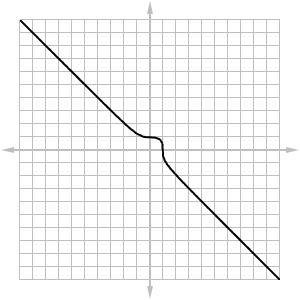
\includegraphics[width=0.6\linewidth]{implicit7}
            \end{center}
      \item $ \sin^2 y + \cos^2 x = 1 $
            \begin{center}
              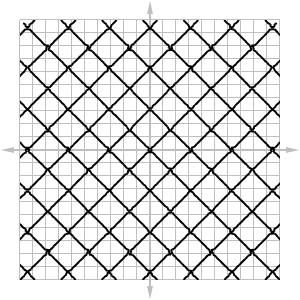
\includegraphics[width=0.6\linewidth]{implicit2}
            \end{center}
      \vfill\null
      \columnbreak
      \item $ x^3 + y^3 = 6xy $ (the folium of Descartes)
            \begin{center}
              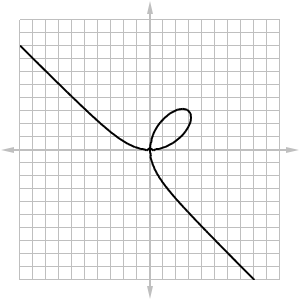
\includegraphics[width=0.6\linewidth]{folium}
            \end{center}
      \item $ y \cos x = 1 + \sin(xy) $
            \begin{center}
              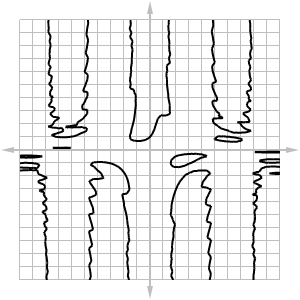
\includegraphics[width=0.6\linewidth]{implicit6}
            \end{center}
      \vfill\null
      \columnbreak
      \item $ x^2 + xy - y^2 = 4 $
            \begin{center}
              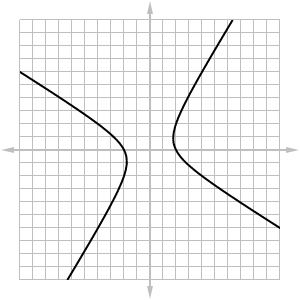
\includegraphics[width=0.6\linewidth]{implicit4}
            \end{center}
      \item $ \frac{1}{x} + \frac{1}{y} = 1 $
            \begin{center}
              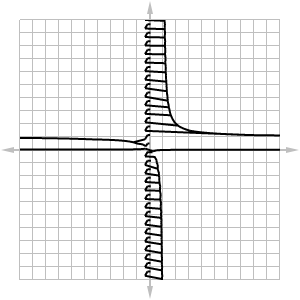
\includegraphics[width=0.6\linewidth]{implicit3}
            \end{center}
      \item $ x^2 y^2 + x \sin y = 4 $
            \begin{center}
              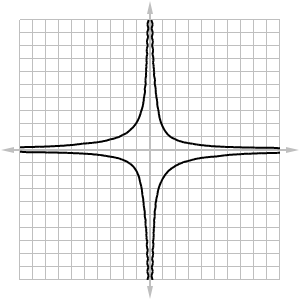
\includegraphics[width=0.6\linewidth]{implicit8}
            \end{center}
      \item $ x^4 y^2 - x^3 y + 2 x y^3 = 0 $
            \begin{center}
              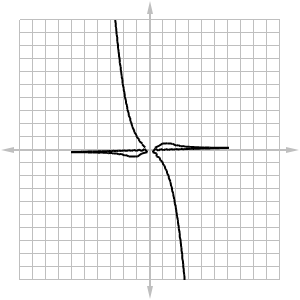
\includegraphics[width=0.6\linewidth]{implicit9}
            \end{center}
      \item $ \tan(x - y) = \frac{y}{1 + x^2} $
            \begin{center}
              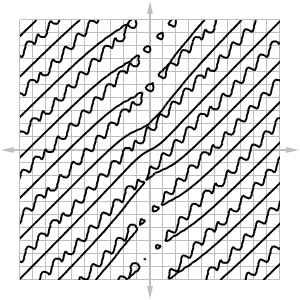
\includegraphics[width=0.6\linewidth]{implicit5}
            \end{center}
      \item $ \sin\left(\frac{x}{y}\right) = \frac{1}{2} $
            \begin{center}
              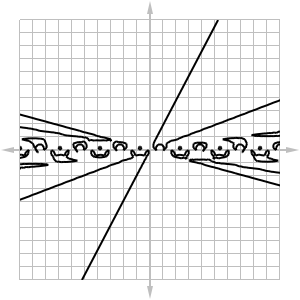
\includegraphics[width=0.6\linewidth]{implicit16}
            \end{center}
    \end{enumerate}
    \end{multicols}
  \item Consider the circle $ x^2 + y^2 = 1 $. Find the equation of the tangent to the curve at $ (\sqrt{2}, \sqrt{2}) $.
  \item The ellipse $ x^2 + 3y^2 = 36 $ has two tangent lines passing through the point $ (12, 3) $. Find both.
        \textit{This question is similar to one from the 2015 Scholarship paper.}
  \begin{multicols}{2}
  \item Find $ x' $ and $ y' $ if $ \ln(y) = \sin(xy) + \frac{x}{y} $.
        \begin{center}
          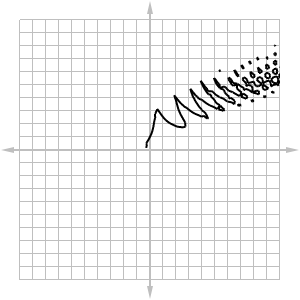
\includegraphics[width=0.6\linewidth]{implicit13}
        \end{center}
  \end{multicols}
  \begin{multicols}{2}
  \item Find $ y'' $ if $ x^4 + y^4 = 16$.
        \begin{center}
          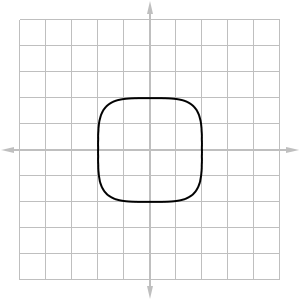
\includegraphics[width=0.6\linewidth]{implicit15}
        \end{center}
  \end{multicols}
  \begin{multicols}{2}
  \item If $ x^2 + xy + y^3 = 1 $, find the value of $ y''' $ at the point where $ x = 1 $.
        \begin{center}
          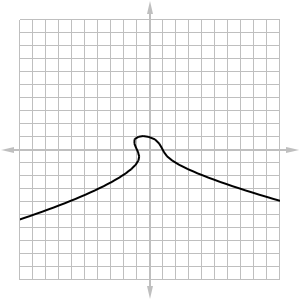
\includegraphics[width=0.6\linewidth]{implicit14}
        \end{center}
  \end{multicols}
  \begin{multicols}{2}
  \item Find a tangent line to the curve $ 2(x^2 + y^2)^2 = 25(x^2 - y^2) $ at the point $ (3, 1) $. This curve is known
        as a lemniscate.
        \begin{center}
          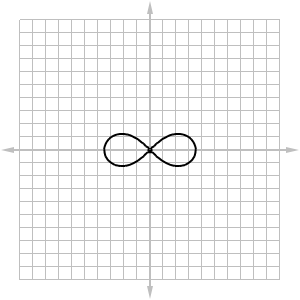
\includegraphics[width=0.6\linewidth]{lemniscate}
        \end{center}
  \end{multicols}
  \begin{multicols}{2}
  \item Find a tangent line to the curve $ y^2(y^2 - 4) = x^2(x^2 - 5) $ at the point $ (0, -2) $. This curve is known
        as a devil's curve.
        \begin{center}
          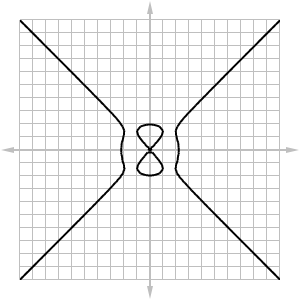
\includegraphics[width=0.6\linewidth]{devilcurve}
        \end{center}
  \end{multicols}
  \item Consider the ellipse $ x^2 - xy + y^2 = 3 $.
    \begin{enumerate}
      \item Find the points where the ellipse crosses the $ x$-axis.
      \item Show that the tangent lines of the curve at these points are parallel.
      \item Find the maximum and minimum points of the curve.
    \end{enumerate}
  \item Consider a circle $ C $ that is tangent to $ 3x + 4y - 12 = 0 $ at $ (0, 3) $ and contains $ (2, -1) $. Set
        up equations that would determine the centre $ (h,k) $ and radius $ r $ of $ C $.
  \item The Bessel function of order 0, $ y = J(x) $, satisfies the equation
        \begin{displaymath}
          xy'' + y' + xy = 2
        \end{displaymath}
        for all values of $ x $. The value of the function at 0 is $ J(0) = 1 $.
    \begin{enumerate}
      \item Find $ J'(0) $.
      \item Use implicit differentiation to find $ J''(0) $.
    \end{enumerate}
  \item Scholarship 2018: Suppose a circle with centre $ O $ is drawn, and a point $ A $ is picked within the circle. Where should a point $ P $ be
        placed on the circumference of the circle such that the interior angle of the triangle $ OAP $ at $ P $ is maximised?
  \item Scholarship 2012: Consider the equation $ x^n = \tan(ny) $, where $ n $ is a constant. Find an expression
        for $ \od{y}{x} $ in terms of $ x $.
  \item Scholarship 2017: The functions $ \sinh $ and $ \cosh $ are defined as follows.
        \begin{align*}
          \sinh x &= \frac{1}{2}\left(e^x - e^{-x}\right),\\
          \cosh x &= \frac{1}{2}\left(e^x + e^{-x}\right).
        \end{align*}
        The inverse function of $ \sinh $ is denoted by $ \sinh^{-1} $. By implicit differentiation, or
        otherwise, show that
        \begin{displaymath}
          \od{}{x} \sinh^{-1} x = \frac{1}{\sqrt{x^2 + 1}}.
        \end{displaymath}
  \item Consider the following family of curves, known as Durer's shell curves (shown here for $ a = 2 $, $ b = 3 $):
        \begin{displaymath}
          (x^2 + xy + ax - b^2)^2 = (b^2 - x^2)(x - y + a)^2.
        \end{displaymath}
        \begin{center}
          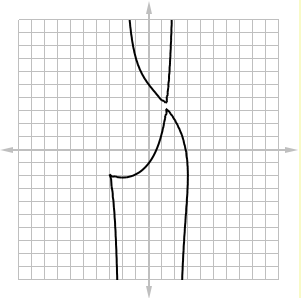
\includegraphics[width=0.3\linewidth]{durer}
        \end{center}
    \begin{enumerate}
      \item For which value(s) of $ b $ does the curve become a straight line?
      \item Suppose that we restrict $ a = \frac{b}{2} $. Find all non-differentiable points on the curve.
    \end{enumerate}
\end{enumerate}

\subsection{References}
For many more examples and exercises, see Stewart, \S2.6. Wikipedia also has a long list of interesting curves
at \url{https://en.wikipedia.org/wiki/List_of_curves}.

For a proof of the implicit function theorem, see Loomis and Sternberg, \S3.11.

This subject properly belongs to the field of differential geometry; see the references for \S9.

\subsection{Homework problems}
\begin{enumerate}
  \item Find $ y' $ in each case:
    \begin{multicols}{3}
    \begin{enumerate}
      \item $ y^2 = x^3 + 3x^2 $\\(Tschirnhausen cubic)
            \begin{center}
              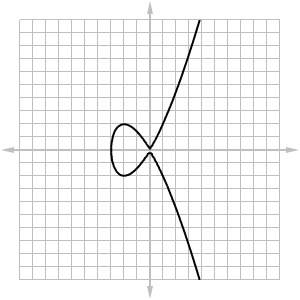
\includegraphics[width=\linewidth]{implicit10}
            \end{center}
      \item $ \sin(x + y) = 2x - 2y $
            \begin{center}
              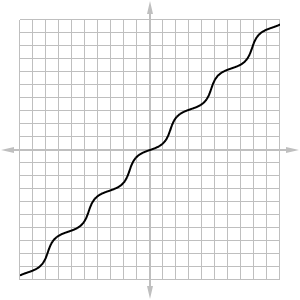
\includegraphics[width=\linewidth]{implicit11}
            \end{center}
      \item $ y^2 = 5x^4 - x^2 $\\(kampyle of Eudoxus)
            \begin{center}
              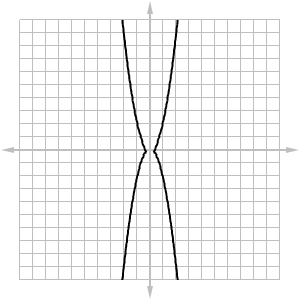
\includegraphics[width=\linewidth]{implicit12}
            \end{center}
    \end{enumerate}
    \end{multicols}
  \item Find the equation of the normal line to the curve $ x^2 + 2xy - y^2 + x = 2 $ at the point $ (1, 2) $.
  \item Show that the sum of the $ x $ and $ y $ intercepts of any tangent line to the curve $ \sqrt{x} + \sqrt{y} = \sqrt{c} $
        is just $ c $.
\end{enumerate}

\section{Geometry of parameterised curves}
In the last section, we tried to describe the geometry of curves that can be described by implicit functions. There is another direction we can
generalise which will give us some similarly nice results.

A very simple example of the technique we want to study can be generted by recalling the definition of the functions $ \sin $ and $ \cos $. For
each angle $ t $ take the line $ \ell (t) $ through $ (0,0) $ which makes an anticlockwise angle $ t $ with the positive $ x$--axis, and call the
intersection point between $ \ell (t) $ and the unit circle $ P = (x,y) $; then set $ \sin t = y $ and $ \cos t = x $.

This definition sets up an exact correspondence between angles $ t $ ($ -\pi \leq t < \pi $) and points $ (x,y) $ on the unit circle ---
for each angle $ t $ we have precisely one point $ (\cos t, \sin t) $ on the circle, and for each point $ (x,y) $ on the circle
there is precisely one number $ t = \arcsin t = \arccos t $.

\begin{figure}
  \centering
  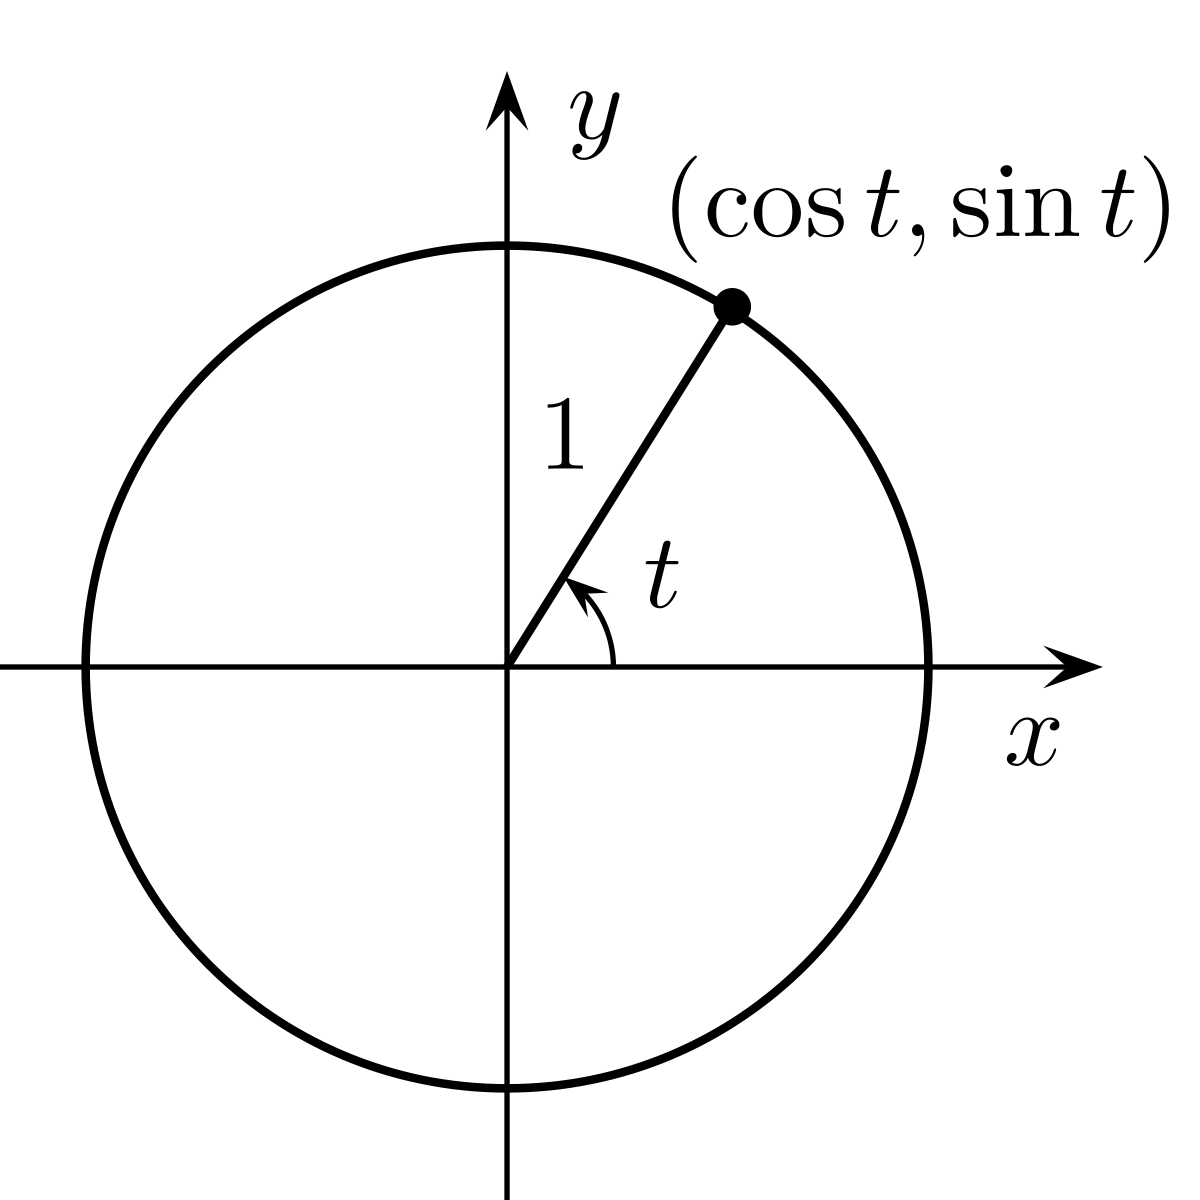
\includegraphics[width=0.2\textwidth]{circle}
  \caption{Parameterisation of the circle.\label{fig:param1}}
\end{figure}

In particular, we can say that the circle is the set of all points $ (x,y) = (\cos t, \sin t) $; and this is just a function (well, a pair
of functions) of one variable --- increasing $ t $ walks around the circle anticlockwise. We can differentiate to find that $ \od{x}{t} = -\sin t $
and $ \od{y}{t} = \cos t $; thus, by the chain rule,
\begin{equation}
  \od{y}{x} = \od{y}{t} \cdot \od{t}{x} = \frac{\cos t}{-\sin t} = -\frac{x}{y}.
\end{equation}

More generally, we want to study curves whose coordinates depend on a single parameter. If $ f $ and $ g $ are
differentiable functions, the curve $ \gamma $ given by
\begin{equation}
  \gamma(t) = (x,y) = (f(t), g(t))
\end{equation}
is called a \emph{parameterised curve}.

Recall that the \emph{implicit function theorem} states (roughly) that every curve can be sliced up into pieces which form the graphs of functions. For
each piece, $ y = g(f^{-1}(x)) $ and so
\begin{displaymath}
  \od{y}{x} = \frac{1}{f'(f^{-1}(x))} \cdot g'(f^{-1}(x)) = \frac{1}{f'(t)} \cdot g'(t) = \frac{1}{\od{x}{t}} \cdot \od{y}{t} = \od{y}{t} \cdot \od{t}{x}.
\end{displaymath}

In order to find the second derivative, we replace $ y $ with $ \od{y}{x} $:
\begin{displaymath}
  \dod[2]{y}{x} = \dod{\od{y}{x}}{x} = \left(\dod{}{t} \dod{y}{x}\right) \cdot \dod{t}{x}.
\end{displaymath}

\subsection{Exercises and Problems}
\begin{enumerate}
  \item In each case find $ \od{y}{x} $.
    \begin{enumerate}
      \item $ x = t\sin t $, $ y = t^2 + t $
      \item $ x = 2 \sec \theta $, $ y = 3\tan \theta $
      \item $ x = \cos \theta $, $ y = \cos 3\theta $
      \item $ x = e^{\sin \theta} $, $ y = e^{\cos \theta} $
    \end{enumerate}
  \item Find the equation of the chord joining the two points $ t = 2 $ and $ t = 4 $ on the
        curve $ (x,y) = (2t - 3, t^3 + 6) $.
  \item Determine the point(s) of intersection of the curves $ \gamma $ and $ \delta $ defined by
        \begin{align*}
          \gamma &: t \mapsto (t^2 - 2, t - 1),\\
          \delta &: t \mapsto (t, 2/t).
        \end{align*}
  \item
    \begin{enumerate}
      \item If $ y = 2t $ and $ x = 4t^2 $ define a curve, what is the gradient $ \od{y}{x} $ in terms of $ t $?
      \item Show that this curve is a parabola.
    \end{enumerate}
  \item A curve has parametric equations $ x = t^2 + 1 $ and $ y = t^3 + 2 $. Find $ \od{y}{x} $ and $ \od[2]{y}{x} $.
  \item Find the equation of the tangent to the curve $ t \mapsto (2x^2 + 1, t^3 - 1) $ at $ t = 2 $.
  \item If $ t \mapsto (x, y) $ is a parametric curve, find an expression for $ \od[3]{y}{x} $ analagous to that found for
        the second derivative.
  \item A curve, called a \textit{witch of Maria Agnesi}, consists of all possible positions of the point $ P $ in
        the diagram below. Graph the curve, show that the curve is given parametrically by $ (x, y) = (2a \cot \theta, 2a \sin^2 \theta) $, and
        find the derivative $ \od{y}{x} $.
        \begin{center}
          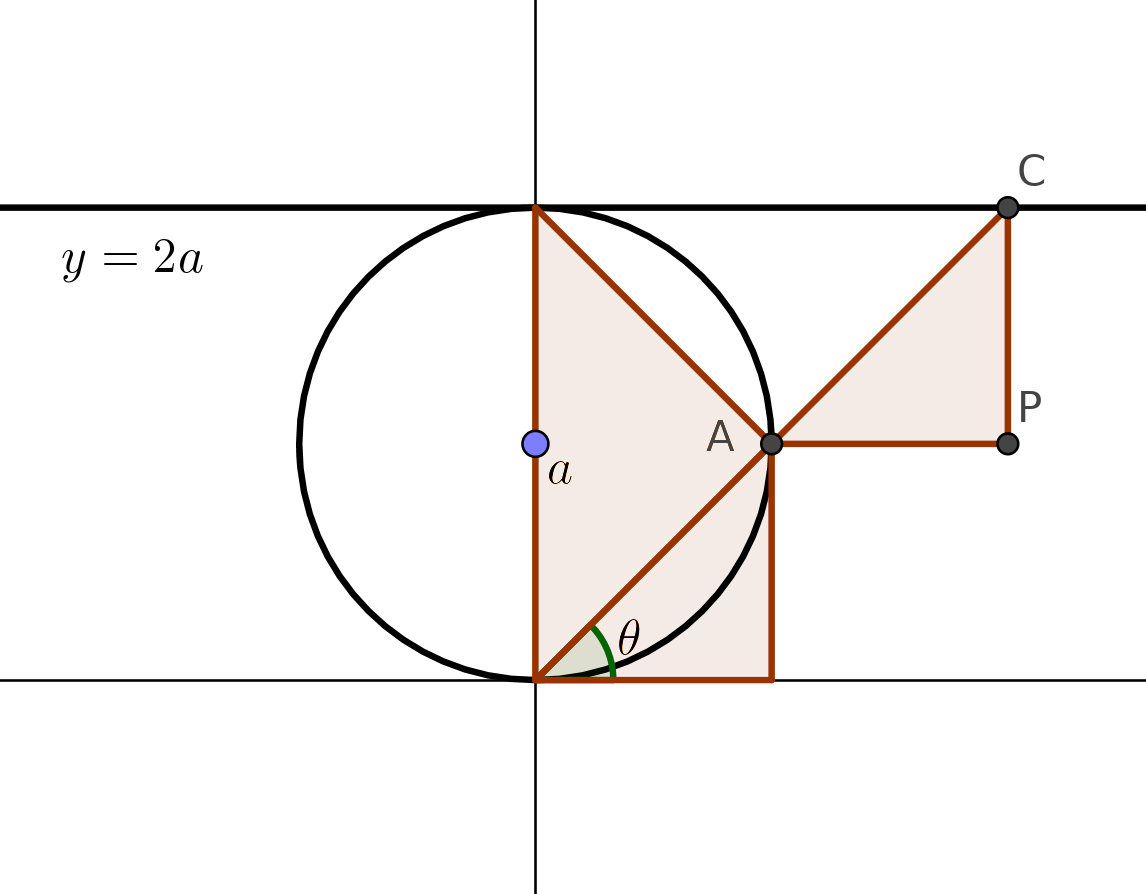
\includegraphics[width=0.5\textwidth]{agnesi-geom}
        \end{center}
  \item A particle moves through space over time; the position of the particle at time $ t $ is
        given by $ (3\sin t, 2\cos t) $ ($ 0 \leq t < 2\pi $).
    \begin{enumerate}
      \item What is the component of the acceleration of the particle in the $ x $ direction at $ t = \pi/4 $?
      \item At what times is the particle stationary in the $ x $ direction?
      \item Is the particle ever momentarily totally stationary?
    \end{enumerate}
  \item Find the rightmost point on the curve $ x = t - t^6 $, $ y = e^t $.
  \item For which values of $ t $ is the curve $ x = \cos 2t $, $ y = 3\cos t $ concave up?
  \item Show that the curve $ \gamma : t \mapsto (\cos t, \sin t \cos t) $ has two tangents at (0,0)
        and find their equations.
  \item
    \begin{enumerate}
      \item Give a second parameterisation of the unit circle $ x^2 + y^2 = 1 $ by considering the set of all lines through $ (-1,0) $.
      \item Give a parameterisation for the cubic $ x^3 - y^2 = 0 $. Find $ \od{y}{x} $ both using implicit differentiation and parametric
            differentiation, and check that the two results agree.
    \end{enumerate}
  \item Scholarship 2000: The piriform is the curve defined by the equation $ 16y^2 = x^3(8-x) $ where $ x \geq 0 $.
    \begin{enumerate}
      \item Show that
            \begin{displaymath}\begin{cases}
              x = 4(1 + \sin \theta)\\
              y = 4(1 + \sin \theta)\cos \theta.
            \end{cases}\end{displaymath}
            are parametric equations for the piriform.
      \item Find $ \od{y}{x} $ in terms of $ \theta $, and show that $ \theta = \frac{\pi}{6} $ is a stationary point of the curve.
    \end{enumerate}
  \item We define a surface $ C $ parametrically in terms of two parameters, $ t $ and $ \theta $:
        \begin{displaymath}
          (x,y,z) = (t, t \cos \theta, t \sin \theta).
        \end{displaymath}
    \begin{enumerate}
      \item Show that the Cartesian equation for this surface is $ x^2 = y^2 + z^2 $. (This is a cone.)
      \item Show that the intersection between $ C $ and the plane $ z = 2 $ is a hyperbola.
      \item For what angle $ \alpha $ does the intersection between $ C $ and the plane parametrically defined by
            \begin{displaymath}
              (x,y,z) = (u\tan \alpha + 1, u, v)
            \end{displaymath}
            (for parameters $ u $ and $ v $) become a parabola? (Hint: $ x = y \tan \alpha + 1 $, and $ z $ is arbitrary.)
    \end{enumerate}
\end{enumerate}

\subsection{References}

\subsection{Homework problems}
\begin{enumerate}
  \item F
\end{enumerate}


\end{document}
